\documentclass[twoside]{book}

% Packages required by doxygen
\usepackage{fixltx2e}
\usepackage{calc}
\usepackage{doxygen}
\usepackage{graphicx}
\usepackage[utf8]{inputenc}
\usepackage{makeidx}
\usepackage{multicol}
\usepackage{multirow}
\PassOptionsToPackage{warn}{textcomp}
\usepackage{textcomp}
\usepackage[nointegrals]{wasysym}
\usepackage[table]{xcolor}

% Font selection
\usepackage[T1]{fontenc}
\usepackage{mathptmx}
\usepackage[scaled=.90]{helvet}
\usepackage{courier}
\usepackage{amssymb}
\usepackage{sectsty}
\renewcommand{\familydefault}{\sfdefault}
\allsectionsfont{%
  \fontseries{bc}\selectfont%
  \color{darkgray}%
}
\renewcommand{\DoxyLabelFont}{%
  \fontseries{bc}\selectfont%
  \color{darkgray}%
}
\newcommand{\+}{\discretionary{\mbox{\scriptsize$\hookleftarrow$}}{}{}}

% Page & text layout
\usepackage{geometry}
\geometry{%
  a4paper,%
  top=2.5cm,%
  bottom=2.5cm,%
  left=2.5cm,%
  right=2.5cm%
}
\tolerance=750
\hfuzz=15pt
\hbadness=750
\setlength{\emergencystretch}{15pt}
\setlength{\parindent}{0cm}
\setlength{\parskip}{0.2cm}
\makeatletter
\renewcommand{\paragraph}{%
  \@startsection{paragraph}{4}{0ex}{-1.0ex}{1.0ex}{%
    \normalfont\normalsize\bfseries\SS@parafont%
  }%
}
\renewcommand{\subparagraph}{%
  \@startsection{subparagraph}{5}{0ex}{-1.0ex}{1.0ex}{%
    \normalfont\normalsize\bfseries\SS@subparafont%
  }%
}
\makeatother

% Headers & footers
\usepackage{fancyhdr}
\pagestyle{fancyplain}
\fancyhead[LE]{\fancyplain{}{\bfseries\thepage}}
\fancyhead[CE]{\fancyplain{}{}}
\fancyhead[RE]{\fancyplain{}{\bfseries\leftmark}}
\fancyhead[LO]{\fancyplain{}{\bfseries\rightmark}}
\fancyhead[CO]{\fancyplain{}{}}
\fancyhead[RO]{\fancyplain{}{\bfseries\thepage}}
\fancyfoot[LE]{\fancyplain{}{}}
\fancyfoot[CE]{\fancyplain{}{}}
\fancyfoot[RE]{\fancyplain{}{\bfseries\scriptsize Generated on Mon Jun 5 2017 20\+:58\+:43 for vinecopulib by Doxygen }}
\fancyfoot[LO]{\fancyplain{}{\bfseries\scriptsize Generated on Mon Jun 5 2017 20\+:58\+:43 for vinecopulib by Doxygen }}
\fancyfoot[CO]{\fancyplain{}{}}
\fancyfoot[RO]{\fancyplain{}{}}
\renewcommand{\footrulewidth}{0.4pt}
\renewcommand{\chaptermark}[1]{%
  \markboth{#1}{}%
}
\renewcommand{\sectionmark}[1]{%
  \markright{\thesection\ #1}%
}

% Indices & bibliography
\usepackage{natbib}
\usepackage[titles]{tocloft}
\setcounter{tocdepth}{3}
\setcounter{secnumdepth}{5}
\makeindex

% Hyperlinks (required, but should be loaded last)
\usepackage{ifpdf}
\ifpdf
  \usepackage[pdftex,pagebackref=true]{hyperref}
\else
  \usepackage[ps2pdf,pagebackref=true]{hyperref}
\fi
\hypersetup{%
  colorlinks=true,%
  linkcolor=blue,%
  citecolor=blue,%
  unicode%
}

% Custom commands
\newcommand{\clearemptydoublepage}{%
  \newpage{\pagestyle{empty}\cleardoublepage}%
}


%===== C O N T E N T S =====

\begin{document}

% Titlepage & ToC
\hypersetup{pageanchor=false,
             bookmarks=true,
             bookmarksnumbered=true,
             pdfencoding=unicode
            }
\pagenumbering{roman}
\begin{titlepage}
\vspace*{7cm}
\begin{center}%
{\Large vinecopulib \\[1ex]\large 0.\+0.\+3 }\\
\vspace*{1cm}
{\large Generated by Doxygen 1.8.7}\\
\vspace*{0.5cm}
{\small Mon Jun 5 2017 20:58:43}\\
\end{center}
\end{titlepage}
\clearemptydoublepage
\tableofcontents
\clearemptydoublepage
\pagenumbering{arabic}
\hypersetup{pageanchor=true}

%--- Begin generated contents ---
\chapter{vinecopulib\+: a C++ library for vine copula modeling}
\label{index}\hypertarget{index}{}\begin{DoxyAuthor}{Authors}
Thomas Nagler and Thibault Vatter
\end{DoxyAuthor}
This is the A\+PI documentation for the vinecopulib C++ library. It provides functionality for statistical dependence modeling with bivariate and vine copulas. For a more high-\/level overview see \href{https://github.com/tvatter/vinecopulib/blob/master/README.md}{\tt R\+E\+A\+D\+ME}.\hypertarget{index_license}{}\section{License}\label{index_license}
The M\+IT License (M\+IT)

Copyright © 2017 Thibault Vatter and Thomas Nagler

Permission is hereby granted, free of charge, to any person obtaining a copy of this software and associated documentation files (the “\+Software”), to deal in the Software without restriction, including without limitation the rights to use, copy, modify, merge, publish, distribute, sublicense, and/or sell copies of the Software, and to permit persons to whom the Software is furnished to do so, subject to the following conditions\+:

The above copyright notice and this permission notice shall be included in all copies or substantial portions of the Software.

T\+HE S\+O\+F\+T\+W\+A\+RE IS P\+R\+O\+V\+I\+D\+ED “\+AS I\+S”, W\+I\+T\+H\+O\+UT W\+A\+R\+R\+A\+N\+TY OF A\+NY K\+I\+ND, E\+X\+P\+R\+E\+SS OR I\+M\+P\+L\+I\+ED, I\+N\+C\+L\+U\+D\+I\+NG B\+UT N\+OT L\+I\+M\+I\+T\+ED TO T\+HE W\+A\+R\+R\+A\+N\+T\+I\+ES OF M\+E\+R\+C\+H\+A\+N\+T\+A\+B\+I\+L\+I\+TY, F\+I\+T\+N\+E\+SS F\+OR A P\+A\+R\+T\+I\+C\+U\+L\+AR P\+U\+R\+P\+O\+SE A\+ND N\+O\+N\+I\+N\+F\+R\+I\+N\+G\+E\+M\+E\+NT. IN NO E\+V\+E\+NT S\+H\+A\+LL T\+HE A\+U\+T\+H\+O\+RS OR C\+O\+P\+Y\+R\+I\+G\+HT H\+O\+L\+D\+E\+RS BE L\+I\+A\+B\+LE F\+OR A\+NY C\+L\+A\+IM, D\+A\+M\+A\+G\+ES OR O\+T\+H\+ER L\+I\+A\+B\+I\+L\+I\+TY, W\+H\+E\+T\+H\+ER IN AN A\+C\+T\+I\+ON OF C\+O\+N\+T\+R\+A\+CT, T\+O\+RT OR O\+T\+H\+E\+R\+W\+I\+SE, A\+R\+I\+S\+I\+NG F\+R\+OM, O\+UT OF OR IN C\+O\+N\+N\+E\+C\+T\+I\+ON W\+I\+TH T\+HE S\+O\+F\+T\+W\+A\+RE OR T\+HE U\+SE OR O\+T\+H\+ER D\+E\+A\+L\+I\+N\+GS IN T\+HE S\+O\+F\+T\+W\+A\+RE. 
\chapter{Namespace Index}
\section{Namespace List}
Here is a list of all documented namespaces with brief descriptions\+:\begin{DoxyCompactList}
\item\contentsline{section}{\hyperlink{namespacetools__eigen}{tools\+\_\+eigen} \\*Tools for working with Eigen types }{\pageref{namespacetools__eigen}}{}
\item\contentsline{section}{\hyperlink{namespacetools__optimization}{tools\+\_\+optimization} \\*Utilities for numerical optimization (based on N\+Lopt) }{\pageref{namespacetools__optimization}}{}
\item\contentsline{section}{\hyperlink{namespacetools__stats}{tools\+\_\+stats} \\*Utilities for statistical analysis }{\pageref{namespacetools__stats}}{}
\item\contentsline{section}{\hyperlink{namespacevinecopulib}{vinecopulib} \\*Tools for bivariate and vine copula modeling }{\pageref{namespacevinecopulib}}{}
\item\contentsline{section}{\hyperlink{namespacevinecopulib_1_1bicop__families}{vinecopulib\+::bicop\+\_\+families} \\*Convenience definitions of sets of bivariate copula families }{\pageref{namespacevinecopulib_1_1bicop__families}}{}
\end{DoxyCompactList}

\chapter{Hierarchical Index}
\section{Class Hierarchy}
This inheritance list is sorted roughly, but not completely, alphabetically\+:\begin{DoxyCompactList}
\item \contentsline{section}{vinecopulib\+:\+:Abstract\+Bicop}{\pageref{classvinecopulib_1_1_abstract_bicop}}{}
\begin{DoxyCompactList}
\item \contentsline{section}{vinecopulib\+:\+:Kernel\+Bicop}{\pageref{classvinecopulib_1_1_kernel_bicop}}{}
\begin{DoxyCompactList}
\item \contentsline{section}{vinecopulib\+:\+:Tll0\+Bicop}{\pageref{classvinecopulib_1_1_tll0_bicop}}{}
\end{DoxyCompactList}
\item \contentsline{section}{vinecopulib\+:\+:Par\+Bicop}{\pageref{classvinecopulib_1_1_par_bicop}}{}
\begin{DoxyCompactList}
\item \contentsline{section}{vinecopulib\+:\+:Archimedean\+Bicop}{\pageref{classvinecopulib_1_1_archimedean_bicop}}{}
\begin{DoxyCompactList}
\item \contentsline{section}{vinecopulib\+:\+:Bb1\+Bicop}{\pageref{classvinecopulib_1_1_bb1_bicop}}{}
\item \contentsline{section}{vinecopulib\+:\+:Bb6\+Bicop}{\pageref{classvinecopulib_1_1_bb6_bicop}}{}
\item \contentsline{section}{vinecopulib\+:\+:Bb7\+Bicop}{\pageref{classvinecopulib_1_1_bb7_bicop}}{}
\item \contentsline{section}{vinecopulib\+:\+:Bb8\+Bicop}{\pageref{classvinecopulib_1_1_bb8_bicop}}{}
\item \contentsline{section}{vinecopulib\+:\+:Clayton\+Bicop}{\pageref{classvinecopulib_1_1_clayton_bicop}}{}
\item \contentsline{section}{vinecopulib\+:\+:Frank\+Bicop}{\pageref{classvinecopulib_1_1_frank_bicop}}{}
\item \contentsline{section}{vinecopulib\+:\+:Gumbel\+Bicop}{\pageref{classvinecopulib_1_1_gumbel_bicop}}{}
\item \contentsline{section}{vinecopulib\+:\+:Joe\+Bicop}{\pageref{classvinecopulib_1_1_joe_bicop}}{}
\end{DoxyCompactList}
\item \contentsline{section}{vinecopulib\+:\+:Elliptical\+Bicop}{\pageref{classvinecopulib_1_1_elliptical_bicop}}{}
\begin{DoxyCompactList}
\item \contentsline{section}{vinecopulib\+:\+:Gaussian\+Bicop}{\pageref{classvinecopulib_1_1_gaussian_bicop}}{}
\item \contentsline{section}{vinecopulib\+:\+:Student\+Bicop}{\pageref{classvinecopulib_1_1_student_bicop}}{}
\end{DoxyCompactList}
\item \contentsline{section}{vinecopulib\+:\+:Indep\+Bicop}{\pageref{classvinecopulib_1_1_indep_bicop}}{}
\end{DoxyCompactList}
\end{DoxyCompactList}
\item \contentsline{section}{vinecopulib\+:\+:Bicop}{\pageref{classvinecopulib_1_1_bicop}}{}
\item \contentsline{section}{vinecopulib\+:\+:Fit\+Controls\+Bicop}{\pageref{classvinecopulib_1_1_fit_controls_bicop}}{}
\begin{DoxyCompactList}
\item \contentsline{section}{vinecopulib\+:\+:Fit\+Controls\+Vinecop}{\pageref{classvinecopulib_1_1_fit_controls_vinecop}}{}
\end{DoxyCompactList}
\item \contentsline{section}{vinecopulib\+:\+:tools\+\_\+interpolation\+:\+:Interpolation\+Grid}{\pageref{classvinecopulib_1_1tools__interpolation_1_1_interpolation_grid}}{}
\item \contentsline{section}{vinecopulib\+:\+:tools\+\_\+optimization\+:\+:N\+Lopt\+Controls}{\pageref{classvinecopulib_1_1tools__optimization_1_1_n_lopt_controls}}{}
\item \contentsline{section}{vinecopulib\+:\+:tools\+\_\+optimization\+:\+:Optimizer}{\pageref{classvinecopulib_1_1tools__optimization_1_1_optimizer}}{}
\item \contentsline{section}{vinecopulib\+:\+:tools\+\_\+optimization\+:\+:Par\+Bicop\+Opt\+Data}{\pageref{structvinecopulib_1_1tools__optimization_1_1_par_bicop_opt_data}}{}
\item \contentsline{section}{vinecopulib\+:\+:R\+Vine\+Matrix}{\pageref{classvinecopulib_1_1_r_vine_matrix}}{}
\item \contentsline{section}{vinecopulib\+:\+:Vinecop}{\pageref{classvinecopulib_1_1_vinecop}}{}
\end{DoxyCompactList}

\chapter{Class Index}
\section{Class List}
Here are the classes, structs, unions and interfaces with brief descriptions\+:\begin{DoxyCompactList}
\item\contentsline{section}{\hyperlink{classvinecopulib_1_1_abstract_bicop}{vinecopulib\+::\+Abstract\+Bicop} \\*An abstract class for bivariate copula families }{\pageref{classvinecopulib_1_1_abstract_bicop}}{}
\item\contentsline{section}{\hyperlink{classvinecopulib_1_1_archimedean_bicop}{vinecopulib\+::\+Archimedean\+Bicop} \\*An abstract class for Archimedean copula families }{\pageref{classvinecopulib_1_1_archimedean_bicop}}{}
\item\contentsline{section}{\hyperlink{classvinecopulib_1_1_bb1_bicop}{vinecopulib\+::\+Bb1\+Bicop} \\*The B\+B1 copula }{\pageref{classvinecopulib_1_1_bb1_bicop}}{}
\item\contentsline{section}{\hyperlink{classvinecopulib_1_1_bb6_bicop}{vinecopulib\+::\+Bb6\+Bicop} \\*The B\+B6 copula }{\pageref{classvinecopulib_1_1_bb6_bicop}}{}
\item\contentsline{section}{\hyperlink{classvinecopulib_1_1_bb7_bicop}{vinecopulib\+::\+Bb7\+Bicop} \\*The B\+B7 copula }{\pageref{classvinecopulib_1_1_bb7_bicop}}{}
\item\contentsline{section}{\hyperlink{classvinecopulib_1_1_bb8_bicop}{vinecopulib\+::\+Bb8\+Bicop} \\*The B\+B8 copula }{\pageref{classvinecopulib_1_1_bb8_bicop}}{}
\item\contentsline{section}{\hyperlink{classvinecopulib_1_1_bicop}{vinecopulib\+::\+Bicop} \\*A class for bivariate copula models }{\pageref{classvinecopulib_1_1_bicop}}{}
\item\contentsline{section}{\hyperlink{classvinecopulib_1_1_clayton_bicop}{vinecopulib\+::\+Clayton\+Bicop} \\*The Clayton copula }{\pageref{classvinecopulib_1_1_clayton_bicop}}{}
\item\contentsline{section}{\hyperlink{classvinecopulib_1_1_elliptical_bicop}{vinecopulib\+::\+Elliptical\+Bicop} \\*An abstract class for elliptical copula families }{\pageref{classvinecopulib_1_1_elliptical_bicop}}{}
\item\contentsline{section}{\hyperlink{classvinecopulib_1_1_frank_bicop}{vinecopulib\+::\+Frank\+Bicop} \\*The Frank copula }{\pageref{classvinecopulib_1_1_frank_bicop}}{}
\item\contentsline{section}{\hyperlink{classvinecopulib_1_1_gaussian_bicop}{vinecopulib\+::\+Gaussian\+Bicop} \\*The Gaussian copula }{\pageref{classvinecopulib_1_1_gaussian_bicop}}{}
\item\contentsline{section}{\hyperlink{classvinecopulib_1_1_gumbel_bicop}{vinecopulib\+::\+Gumbel\+Bicop} \\*The Gumbel copula }{\pageref{classvinecopulib_1_1_gumbel_bicop}}{}
\item\contentsline{section}{\hyperlink{classvinecopulib_1_1_indep_bicop}{vinecopulib\+::\+Indep\+Bicop} \\*The independence copula }{\pageref{classvinecopulib_1_1_indep_bicop}}{}
\item\contentsline{section}{\hyperlink{classvinecopulib_1_1_joe_bicop}{vinecopulib\+::\+Joe\+Bicop} \\*The Joe copula }{\pageref{classvinecopulib_1_1_joe_bicop}}{}
\item\contentsline{section}{\hyperlink{classvinecopulib_1_1_kernel_bicop}{vinecopulib\+::\+Kernel\+Bicop} \\*An abstract class for kernel copulas }{\pageref{classvinecopulib_1_1_kernel_bicop}}{}
\item\contentsline{section}{\hyperlink{classtools__optimization_1_1_n_lopt_controls}{tools\+\_\+optimization\+::\+N\+Lopt\+Controls} \\*A class for the controls to N\+Lopt }{\pageref{classtools__optimization_1_1_n_lopt_controls}}{}
\item\contentsline{section}{\hyperlink{classtools__optimization_1_1_optimizer}{tools\+\_\+optimization\+::\+Optimizer} \\*A class for optimization (wrapping N\+Lopt) }{\pageref{classtools__optimization_1_1_optimizer}}{}
\item\contentsline{section}{\hyperlink{classvinecopulib_1_1_par_bicop}{vinecopulib\+::\+Par\+Bicop} \\*An abstract class for parametric copula families }{\pageref{classvinecopulib_1_1_par_bicop}}{}
\item\contentsline{section}{\hyperlink{structtools__optimization_1_1_par_bicop_opt_data}{tools\+\_\+optimization\+::\+Par\+Bicop\+Opt\+Data} \\*A helper struct for (profile) maximum likelihood estimation }{\pageref{structtools__optimization_1_1_par_bicop_opt_data}}{}
\item\contentsline{section}{\hyperlink{classvinecopulib_1_1_r_vine_matrix}{vinecopulib\+::\+R\+Vine\+Matrix} \\*A class for regular vine matrices }{\pageref{classvinecopulib_1_1_r_vine_matrix}}{}
\item\contentsline{section}{\hyperlink{classvinecopulib_1_1_student_bicop}{vinecopulib\+::\+Student\+Bicop} \\*The Student t copula }{\pageref{classvinecopulib_1_1_student_bicop}}{}
\item\contentsline{section}{\hyperlink{classvinecopulib_1_1_trafokernel_bicop}{vinecopulib\+::\+Trafokernel\+Bicop} \\*The transformation local-\/constant likelihood estimator }{\pageref{classvinecopulib_1_1_trafokernel_bicop}}{}
\item\contentsline{section}{\hyperlink{classvinecopulib_1_1_vinecop}{vinecopulib\+::\+Vinecop} \\*A class for vine copula models }{\pageref{classvinecopulib_1_1_vinecop}}{}
\end{DoxyCompactList}

\chapter{File Index}
\section{File List}
Here is a list of all documented files with brief descriptions\+:\begin{DoxyCompactList}
\item\contentsline{section}{/home/n5/dev/cpp/vinecopulib/include/{\bfseries bicop.\+hpp} }{\pageref{bicop_8hpp}}{}
\item\contentsline{section}{/home/n5/dev/cpp/vinecopulib/include/{\bfseries bicop\+\_\+archimedean.\+hpp} }{\pageref{bicop__archimedean_8hpp}}{}
\item\contentsline{section}{/home/n5/dev/cpp/vinecopulib/include/{\bfseries bicop\+\_\+bb1.\+hpp} }{\pageref{bicop__bb1_8hpp}}{}
\item\contentsline{section}{/home/n5/dev/cpp/vinecopulib/include/{\bfseries bicop\+\_\+bb6.\+hpp} }{\pageref{bicop__bb6_8hpp}}{}
\item\contentsline{section}{/home/n5/dev/cpp/vinecopulib/include/{\bfseries bicop\+\_\+bb7.\+hpp} }{\pageref{bicop__bb7_8hpp}}{}
\item\contentsline{section}{/home/n5/dev/cpp/vinecopulib/include/{\bfseries bicop\+\_\+bb8.\+hpp} }{\pageref{bicop__bb8_8hpp}}{}
\item\contentsline{section}{/home/n5/dev/cpp/vinecopulib/include/{\bfseries bicop\+\_\+class.\+hpp} }{\pageref{bicop__class_8hpp}}{}
\item\contentsline{section}{/home/n5/dev/cpp/vinecopulib/include/{\bfseries bicop\+\_\+clayton.\+hpp} }{\pageref{bicop__clayton_8hpp}}{}
\item\contentsline{section}{/home/n5/dev/cpp/vinecopulib/include/{\bfseries bicop\+\_\+elliptical.\+hpp} }{\pageref{bicop__elliptical_8hpp}}{}
\item\contentsline{section}{/home/n5/dev/cpp/vinecopulib/include/{\bfseries bicop\+\_\+frank.\+hpp} }{\pageref{bicop__frank_8hpp}}{}
\item\contentsline{section}{/home/n5/dev/cpp/vinecopulib/include/{\bfseries bicop\+\_\+gauss.\+hpp} }{\pageref{bicop__gauss_8hpp}}{}
\item\contentsline{section}{/home/n5/dev/cpp/vinecopulib/include/{\bfseries bicop\+\_\+gumbel.\+hpp} }{\pageref{bicop__gumbel_8hpp}}{}
\item\contentsline{section}{/home/n5/dev/cpp/vinecopulib/include/{\bfseries bicop\+\_\+indep.\+hpp} }{\pageref{bicop__indep_8hpp}}{}
\item\contentsline{section}{/home/n5/dev/cpp/vinecopulib/include/{\bfseries bicop\+\_\+joe.\+hpp} }{\pageref{bicop__joe_8hpp}}{}
\item\contentsline{section}{/home/n5/dev/cpp/vinecopulib/include/{\bfseries bicop\+\_\+kernel.\+hpp} }{\pageref{bicop__kernel_8hpp}}{}
\item\contentsline{section}{/home/n5/dev/cpp/vinecopulib/include/{\bfseries bicop\+\_\+parametric.\+hpp} }{\pageref{bicop__parametric_8hpp}}{}
\item\contentsline{section}{/home/n5/dev/cpp/vinecopulib/include/{\bfseries bicop\+\_\+student.\+hpp} }{\pageref{bicop__student_8hpp}}{}
\item\contentsline{section}{/home/n5/dev/cpp/vinecopulib/include/{\bfseries bicop\+\_\+trafokernel.\+hpp} }{\pageref{bicop__trafokernel_8hpp}}{}
\item\contentsline{section}{/home/n5/dev/cpp/vinecopulib/include/{\bfseries c\+\_\+tools.\+h} }{\pageref{c__tools_8h}}{}
\item\contentsline{section}{/home/n5/dev/cpp/vinecopulib/include/{\bfseries distribution\+\_\+tools.\+hpp} }{\pageref{distribution__tools_8hpp}}{}
\item\contentsline{section}{/home/n5/dev/cpp/vinecopulib/include/{\bfseries git\+\_\+revision.\+h} }{\pageref{git__revision_8h}}{}
\item\contentsline{section}{/home/n5/dev/cpp/vinecopulib/include/{\bfseries integration\+\_\+tools.\+hpp} }{\pageref{integration__tools_8hpp}}{}
\item\contentsline{section}{/home/n5/dev/cpp/vinecopulib/include/{\bfseries interpolation\+\_\+grid.\+hpp} }{\pageref{interpolation__grid_8hpp}}{}
\item\contentsline{section}{/home/n5/dev/cpp/vinecopulib/include/\hyperlink{mainpage_8h}{mainpage.\+h} \\*Api\+\_\+docs }{\pageref{mainpage_8h}}{}
\item\contentsline{section}{/home/n5/dev/cpp/vinecopulib/include/{\bfseries optimization\+\_\+tools.\+hpp} }{\pageref{optimization__tools_8hpp}}{}
\item\contentsline{section}{/home/n5/dev/cpp/vinecopulib/include/{\bfseries rvine\+\_\+matrix.\+hpp} }{\pageref{rvine__matrix_8hpp}}{}
\item\contentsline{section}{/home/n5/dev/cpp/vinecopulib/include/{\bfseries structselect\+\_\+tools.\+hpp} }{\pageref{structselect__tools_8hpp}}{}
\item\contentsline{section}{/home/n5/dev/cpp/vinecopulib/include/{\bfseries vinecop\+\_\+class.\+hpp} }{\pageref{vinecop__class_8hpp}}{}
\end{DoxyCompactList}

\chapter{Namespace Documentation}
\hypertarget{namespacevinecopulib}{}\section{vinecopulib Namespace Reference}
\label{namespacevinecopulib}\index{vinecopulib@{vinecopulib}}


Tools for bivariate and vine copula modeling.  


\subsection*{Namespaces}
\begin{DoxyCompactItemize}
\item 
 \hyperlink{namespacevinecopulib_1_1bicop__families}{bicop\+\_\+families}
\begin{DoxyCompactList}\small\item\em Convenience definitions of sets of bivariate copula families. \end{DoxyCompactList}\item 
 \hyperlink{namespacevinecopulib_1_1tools__eigen}{tools\+\_\+eigen}
\begin{DoxyCompactList}\small\item\em Tools for working with Eigen types. \end{DoxyCompactList}\item 
 \hyperlink{namespacevinecopulib_1_1tools__optimization}{tools\+\_\+optimization}
\begin{DoxyCompactList}\small\item\em Utilities for numerical optimization (based on N\+Lopt) \end{DoxyCompactList}\item 
 \hyperlink{namespacevinecopulib_1_1tools__stats}{tools\+\_\+stats}
\begin{DoxyCompactList}\small\item\em Utilities for statistical analysis. \end{DoxyCompactList}\end{DoxyCompactItemize}
\subsection*{Classes}
\begin{DoxyCompactItemize}
\item 
class \hyperlink{classvinecopulib_1_1_abstract_bicop}{Abstract\+Bicop}
\begin{DoxyCompactList}\small\item\em An abstract class for bivariate copula families. \end{DoxyCompactList}\item 
class \hyperlink{classvinecopulib_1_1_archimedean_bicop}{Archimedean\+Bicop}
\begin{DoxyCompactList}\small\item\em An abstract class for Archimedean copula families. \end{DoxyCompactList}\item 
class \hyperlink{classvinecopulib_1_1_bb1_bicop}{Bb1\+Bicop}
\begin{DoxyCompactList}\small\item\em The B\+B1 copula. \end{DoxyCompactList}\item 
class \hyperlink{classvinecopulib_1_1_bb6_bicop}{Bb6\+Bicop}
\begin{DoxyCompactList}\small\item\em The B\+B6 copula. \end{DoxyCompactList}\item 
class \hyperlink{classvinecopulib_1_1_bb7_bicop}{Bb7\+Bicop}
\begin{DoxyCompactList}\small\item\em The B\+B7 copula. \end{DoxyCompactList}\item 
class \hyperlink{classvinecopulib_1_1_bb8_bicop}{Bb8\+Bicop}
\begin{DoxyCompactList}\small\item\em The B\+B8 copula. \end{DoxyCompactList}\item 
class \hyperlink{classvinecopulib_1_1_bicop}{Bicop}
\begin{DoxyCompactList}\small\item\em A class for bivariate copula models. \end{DoxyCompactList}\item 
class \hyperlink{classvinecopulib_1_1_clayton_bicop}{Clayton\+Bicop}
\begin{DoxyCompactList}\small\item\em The Clayton copula. \end{DoxyCompactList}\item 
class \hyperlink{classvinecopulib_1_1_elliptical_bicop}{Elliptical\+Bicop}
\begin{DoxyCompactList}\small\item\em An abstract class for elliptical copula families. \end{DoxyCompactList}\item 
class \hyperlink{classvinecopulib_1_1_fit_controls_bicop}{Fit\+Controls\+Bicop}
\begin{DoxyCompactList}\small\item\em A class for controlling fit of bivariate copula models. \end{DoxyCompactList}\item 
class \hyperlink{classvinecopulib_1_1_fit_controls_vinecop}{Fit\+Controls\+Vinecop}
\begin{DoxyCompactList}\small\item\em A class for controlling fit of bivariate copula models. \end{DoxyCompactList}\item 
class \hyperlink{classvinecopulib_1_1_frank_bicop}{Frank\+Bicop}
\begin{DoxyCompactList}\small\item\em The Frank copula. \end{DoxyCompactList}\item 
class \hyperlink{classvinecopulib_1_1_gaussian_bicop}{Gaussian\+Bicop}
\begin{DoxyCompactList}\small\item\em The Gaussian copula. \end{DoxyCompactList}\item 
class \hyperlink{classvinecopulib_1_1_gumbel_bicop}{Gumbel\+Bicop}
\begin{DoxyCompactList}\small\item\em The Gumbel copula. \end{DoxyCompactList}\item 
class \hyperlink{classvinecopulib_1_1_indep_bicop}{Indep\+Bicop}
\begin{DoxyCompactList}\small\item\em The independence copula. \end{DoxyCompactList}\item 
class \hyperlink{classvinecopulib_1_1_joe_bicop}{Joe\+Bicop}
\begin{DoxyCompactList}\small\item\em The Joe copula. \end{DoxyCompactList}\item 
class \hyperlink{classvinecopulib_1_1_kernel_bicop}{Kernel\+Bicop}
\begin{DoxyCompactList}\small\item\em An abstract class for kernel copulas. \end{DoxyCompactList}\item 
class \hyperlink{classvinecopulib_1_1_par_bicop}{Par\+Bicop}
\begin{DoxyCompactList}\small\item\em An abstract class for parametric copula families. \end{DoxyCompactList}\item 
class \hyperlink{classvinecopulib_1_1_r_vine_matrix}{R\+Vine\+Matrix}
\begin{DoxyCompactList}\small\item\em A class for regular vine matrices. \end{DoxyCompactList}\item 
class \hyperlink{classvinecopulib_1_1_student_bicop}{Student\+Bicop}
\begin{DoxyCompactList}\small\item\em The Student t copula. \end{DoxyCompactList}\item 
class \hyperlink{classvinecopulib_1_1_tll0_bicop}{Tll0\+Bicop}
\begin{DoxyCompactList}\small\item\em The transformation local-\/constant likelihood estimator. \end{DoxyCompactList}\item 
class \hyperlink{classvinecopulib_1_1_vinecop}{Vinecop}
\begin{DoxyCompactList}\small\item\em A class for vine copula models. \end{DoxyCompactList}\end{DoxyCompactItemize}
\subsection*{Typedefs}
\begin{DoxyCompactItemize}
\item 
typedef std\+::shared\+\_\+ptr$<$ \hyperlink{classvinecopulib_1_1_abstract_bicop}{Abstract\+Bicop} $>$ \hyperlink{namespacevinecopulib_afd73d02952b845883499cbbda1996204}{Bicop\+Ptr}\hypertarget{namespacevinecopulib_afd73d02952b845883499cbbda1996204}{}\label{namespacevinecopulib_afd73d02952b845883499cbbda1996204}

\begin{DoxyCompactList}\small\item\em A shared pointer to an object of class Abstrac\+Bicop. \end{DoxyCompactList}\end{DoxyCompactItemize}
\subsection*{Enumerations}
\begin{DoxyCompactItemize}
\item 
enum \hyperlink{namespacevinecopulib_a42e95cc06d33896199caab0c11ad44f3}{Bicop\+Family} \{ \\*
\hyperlink{namespacevinecopulib_a42e95cc06d33896199caab0c11ad44f3af49b022096e968010a7b9bd941805a65}{Bicop\+Family\+::indep}, 
\\*
\hyperlink{namespacevinecopulib_a42e95cc06d33896199caab0c11ad44f3a304e2a3b544f6b9f267a151e1bcee487}{Bicop\+Family\+::gaussian}, 
\\*
\hyperlink{namespacevinecopulib_a42e95cc06d33896199caab0c11ad44f3acd73502828457d15655bbd7a63fb0bc8}{Bicop\+Family\+::student}, 
\\*
\hyperlink{namespacevinecopulib_a42e95cc06d33896199caab0c11ad44f3ad0b8c94bb241f6f7a4b96cd6d3e26c36}{Bicop\+Family\+::clayton}, 
\\*
\hyperlink{namespacevinecopulib_a42e95cc06d33896199caab0c11ad44f3a7bfb9d9ee5abbfa800e56bbe62db9bbe}{Bicop\+Family\+::gumbel}, 
\\*
\hyperlink{namespacevinecopulib_a42e95cc06d33896199caab0c11ad44f3a26253c50741faa9c2e2b836773c69fe6}{Bicop\+Family\+::frank}, 
\\*
\hyperlink{namespacevinecopulib_a42e95cc06d33896199caab0c11ad44f3a8ff32489f92f33416694be8fdc2d4c22}{Bicop\+Family\+::joe}, 
\\*
\hyperlink{namespacevinecopulib_a42e95cc06d33896199caab0c11ad44f3a8a2e0a5eece6b7020e5308bcd0df4aa3}{Bicop\+Family\+::bb1}, 
\\*
\hyperlink{namespacevinecopulib_a42e95cc06d33896199caab0c11ad44f3aa2d33c13012f342a80bdc94b60538c68}{Bicop\+Family\+::bb6}, 
\\*
\hyperlink{namespacevinecopulib_a42e95cc06d33896199caab0c11ad44f3ac9e791d6604a5fcc1f4e6ad574f43328}{Bicop\+Family\+::bb7}, 
\\*
\hyperlink{namespacevinecopulib_a42e95cc06d33896199caab0c11ad44f3adf8b15ba30764e3b9ce084c11336603a}{Bicop\+Family\+::bb8}, 
\\*
\hyperlink{namespacevinecopulib_a42e95cc06d33896199caab0c11ad44f3acd36652e61e82e7935de462b329cc8e6}{Bicop\+Family\+::tll0}
 \}\begin{DoxyCompactList}\small\item\em A bivariate copula family identifier. \end{DoxyCompactList}
\end{DoxyCompactItemize}
\subsection*{Functions}
\begin{DoxyCompactItemize}
\item 
std\+::string \hyperlink{namespacevinecopulib_ac46553ae5f99072f65e9d3254d2c526d}{get\+\_\+family\+\_\+name} (\hyperlink{namespacevinecopulib_a42e95cc06d33896199caab0c11ad44f3}{Bicop\+Family} family)
\end{DoxyCompactItemize}


\subsection{Detailed Description}
Tools for bivariate and vine copula modeling. 

\subsection{Enumeration Type Documentation}
\index{vinecopulib@{vinecopulib}!Bicop\+Family@{Bicop\+Family}}
\index{Bicop\+Family@{Bicop\+Family}!vinecopulib@{vinecopulib}}
\subsubsection[{\texorpdfstring{Bicop\+Family}{BicopFamily}}]{\setlength{\rightskip}{0pt plus 5cm}enum {\bf vinecopulib\+::\+Bicop\+Family}\hspace{0.3cm}{\ttfamily [strong]}}\hypertarget{namespacevinecopulib_a42e95cc06d33896199caab0c11ad44f3}{}\label{namespacevinecopulib_a42e95cc06d33896199caab0c11ad44f3}


A bivariate copula family identifier. 

\begin{Desc}
\item[Enumerator]\par
\begin{description}
\index{indep@{indep}!vinecopulib@{vinecopulib}}\index{vinecopulib@{vinecopulib}!indep@{indep}}\item[{\em 
indep\hypertarget{namespacevinecopulib_a42e95cc06d33896199caab0c11ad44f3af49b022096e968010a7b9bd941805a65}{}\label{namespacevinecopulib_a42e95cc06d33896199caab0c11ad44f3af49b022096e968010a7b9bd941805a65}
}]Independence copula. \index{gaussian@{gaussian}!vinecopulib@{vinecopulib}}\index{vinecopulib@{vinecopulib}!gaussian@{gaussian}}\item[{\em 
gaussian\hypertarget{namespacevinecopulib_a42e95cc06d33896199caab0c11ad44f3a304e2a3b544f6b9f267a151e1bcee487}{}\label{namespacevinecopulib_a42e95cc06d33896199caab0c11ad44f3a304e2a3b544f6b9f267a151e1bcee487}
}]Gaussian copula. \index{student@{student}!vinecopulib@{vinecopulib}}\index{vinecopulib@{vinecopulib}!student@{student}}\item[{\em 
student\hypertarget{namespacevinecopulib_a42e95cc06d33896199caab0c11ad44f3acd73502828457d15655bbd7a63fb0bc8}{}\label{namespacevinecopulib_a42e95cc06d33896199caab0c11ad44f3acd73502828457d15655bbd7a63fb0bc8}
}]Student t copula. \index{clayton@{clayton}!vinecopulib@{vinecopulib}}\index{vinecopulib@{vinecopulib}!clayton@{clayton}}\item[{\em 
clayton\hypertarget{namespacevinecopulib_a42e95cc06d33896199caab0c11ad44f3ad0b8c94bb241f6f7a4b96cd6d3e26c36}{}\label{namespacevinecopulib_a42e95cc06d33896199caab0c11ad44f3ad0b8c94bb241f6f7a4b96cd6d3e26c36}
}]Clayton copula. \index{gumbel@{gumbel}!vinecopulib@{vinecopulib}}\index{vinecopulib@{vinecopulib}!gumbel@{gumbel}}\item[{\em 
gumbel\hypertarget{namespacevinecopulib_a42e95cc06d33896199caab0c11ad44f3a7bfb9d9ee5abbfa800e56bbe62db9bbe}{}\label{namespacevinecopulib_a42e95cc06d33896199caab0c11ad44f3a7bfb9d9ee5abbfa800e56bbe62db9bbe}
}]Gumbel copula. \index{frank@{frank}!vinecopulib@{vinecopulib}}\index{vinecopulib@{vinecopulib}!frank@{frank}}\item[{\em 
frank\hypertarget{namespacevinecopulib_a42e95cc06d33896199caab0c11ad44f3a26253c50741faa9c2e2b836773c69fe6}{}\label{namespacevinecopulib_a42e95cc06d33896199caab0c11ad44f3a26253c50741faa9c2e2b836773c69fe6}
}]Frank copula. \index{joe@{joe}!vinecopulib@{vinecopulib}}\index{vinecopulib@{vinecopulib}!joe@{joe}}\item[{\em 
joe\hypertarget{namespacevinecopulib_a42e95cc06d33896199caab0c11ad44f3a8ff32489f92f33416694be8fdc2d4c22}{}\label{namespacevinecopulib_a42e95cc06d33896199caab0c11ad44f3a8ff32489f92f33416694be8fdc2d4c22}
}]Joe copula. \index{bb1@{bb1}!vinecopulib@{vinecopulib}}\index{vinecopulib@{vinecopulib}!bb1@{bb1}}\item[{\em 
bb1\hypertarget{namespacevinecopulib_a42e95cc06d33896199caab0c11ad44f3a8a2e0a5eece6b7020e5308bcd0df4aa3}{}\label{namespacevinecopulib_a42e95cc06d33896199caab0c11ad44f3a8a2e0a5eece6b7020e5308bcd0df4aa3}
}]B\+B1 copula. \index{bb6@{bb6}!vinecopulib@{vinecopulib}}\index{vinecopulib@{vinecopulib}!bb6@{bb6}}\item[{\em 
bb6\hypertarget{namespacevinecopulib_a42e95cc06d33896199caab0c11ad44f3aa2d33c13012f342a80bdc94b60538c68}{}\label{namespacevinecopulib_a42e95cc06d33896199caab0c11ad44f3aa2d33c13012f342a80bdc94b60538c68}
}]B\+B6 copula. \index{bb7@{bb7}!vinecopulib@{vinecopulib}}\index{vinecopulib@{vinecopulib}!bb7@{bb7}}\item[{\em 
bb7\hypertarget{namespacevinecopulib_a42e95cc06d33896199caab0c11ad44f3ac9e791d6604a5fcc1f4e6ad574f43328}{}\label{namespacevinecopulib_a42e95cc06d33896199caab0c11ad44f3ac9e791d6604a5fcc1f4e6ad574f43328}
}]B\+B7 copula. \index{bb8@{bb8}!vinecopulib@{vinecopulib}}\index{vinecopulib@{vinecopulib}!bb8@{bb8}}\item[{\em 
bb8\hypertarget{namespacevinecopulib_a42e95cc06d33896199caab0c11ad44f3adf8b15ba30764e3b9ce084c11336603a}{}\label{namespacevinecopulib_a42e95cc06d33896199caab0c11ad44f3adf8b15ba30764e3b9ce084c11336603a}
}]B\+B8 copula. \index{tll0@{tll0}!vinecopulib@{vinecopulib}}\index{vinecopulib@{vinecopulib}!tll0@{tll0}}\item[{\em 
tll0\hypertarget{namespacevinecopulib_a42e95cc06d33896199caab0c11ad44f3acd36652e61e82e7935de462b329cc8e6}{}\label{namespacevinecopulib_a42e95cc06d33896199caab0c11ad44f3acd36652e61e82e7935de462b329cc8e6}
}]Transformation local-\/constant likelihood kernel estimator. \end{description}
\end{Desc}


\subsection{Function Documentation}
\index{vinecopulib@{vinecopulib}!get\+\_\+family\+\_\+name@{get\+\_\+family\+\_\+name}}
\index{get\+\_\+family\+\_\+name@{get\+\_\+family\+\_\+name}!vinecopulib@{vinecopulib}}
\subsubsection[{\texorpdfstring{get\+\_\+family\+\_\+name(\+Bicop\+Family family)}{get_family_name(BicopFamily family)}}]{\setlength{\rightskip}{0pt plus 5cm}std\+::string vinecopulib\+::get\+\_\+family\+\_\+name (
\begin{DoxyParamCaption}
\item[{{\bf Bicop\+Family}}]{family}
\end{DoxyParamCaption}
)}\hypertarget{namespacevinecopulib_ac46553ae5f99072f65e9d3254d2c526d}{}\label{namespacevinecopulib_ac46553ae5f99072f65e9d3254d2c526d}
converts a Bicop\+Family into a string with its name. 
\begin{DoxyParams}{Parameters}
{\em family} & the family. \\
\hline
\end{DoxyParams}

\hypertarget{namespacevinecopulib_1_1bicop__families}{}\section{vinecopulib\+:\+:bicop\+\_\+families Namespace Reference}
\label{namespacevinecopulib_1_1bicop__families}\index{vinecopulib\+::bicop\+\_\+families@{vinecopulib\+::bicop\+\_\+families}}


Convenience definitions of sets of bivariate copula families.  


\subsection*{Variables}
\begin{DoxyCompactItemize}
\item 
const std\+::vector$<$ \hyperlink{namespacevinecopulib_a42e95cc06d33896199caab0c11ad44f3}{Bicop\+Family} $>$ \hyperlink{namespacevinecopulib_1_1bicop__families_a5214a513f41ec23b74782aab96ea6774}{all}\hypertarget{namespacevinecopulib_1_1bicop__families_a5214a513f41ec23b74782aab96ea6774}{}\label{namespacevinecopulib_1_1bicop__families_a5214a513f41ec23b74782aab96ea6774}

\begin{DoxyCompactList}\small\item\em All implemented families. \end{DoxyCompactList}\item 
const std\+::vector$<$ \hyperlink{namespacevinecopulib_a42e95cc06d33896199caab0c11ad44f3}{Bicop\+Family} $>$ \hyperlink{namespacevinecopulib_1_1bicop__families_a76d66bb6cb03ae4de1cef3d1ed70ac16}{parametric}\hypertarget{namespacevinecopulib_1_1bicop__families_a76d66bb6cb03ae4de1cef3d1ed70ac16}{}\label{namespacevinecopulib_1_1bicop__families_a76d66bb6cb03ae4de1cef3d1ed70ac16}

\begin{DoxyCompactList}\small\item\em All parametric families. \end{DoxyCompactList}\item 
const std\+::vector$<$ \hyperlink{namespacevinecopulib_a42e95cc06d33896199caab0c11ad44f3}{Bicop\+Family} $>$ \hyperlink{namespacevinecopulib_1_1bicop__families_a01c7c990cc34b1b74d115858a52fcdc5}{nonparametric}\hypertarget{namespacevinecopulib_1_1bicop__families_a01c7c990cc34b1b74d115858a52fcdc5}{}\label{namespacevinecopulib_1_1bicop__families_a01c7c990cc34b1b74d115858a52fcdc5}

\begin{DoxyCompactList}\small\item\em All nonparametric families. \end{DoxyCompactList}\item 
const std\+::vector$<$ \hyperlink{namespacevinecopulib_a42e95cc06d33896199caab0c11ad44f3}{Bicop\+Family} $>$ \hyperlink{namespacevinecopulib_1_1bicop__families_aba503484b0a13cfb0e67c026e2f295d4}{one\+\_\+par}\hypertarget{namespacevinecopulib_1_1bicop__families_aba503484b0a13cfb0e67c026e2f295d4}{}\label{namespacevinecopulib_1_1bicop__families_aba503484b0a13cfb0e67c026e2f295d4}

\begin{DoxyCompactList}\small\item\em All one-\/parameter families. \end{DoxyCompactList}\item 
const std\+::vector$<$ \hyperlink{namespacevinecopulib_a42e95cc06d33896199caab0c11ad44f3}{Bicop\+Family} $>$ \hyperlink{namespacevinecopulib_1_1bicop__families_ad5871c39b4ee62bd44fa851d7d70c7ca}{two\+\_\+par}\hypertarget{namespacevinecopulib_1_1bicop__families_ad5871c39b4ee62bd44fa851d7d70c7ca}{}\label{namespacevinecopulib_1_1bicop__families_ad5871c39b4ee62bd44fa851d7d70c7ca}

\begin{DoxyCompactList}\small\item\em All two-\/parameter families. \end{DoxyCompactList}\item 
const std\+::vector$<$ \hyperlink{namespacevinecopulib_a42e95cc06d33896199caab0c11ad44f3}{Bicop\+Family} $>$ \hyperlink{namespacevinecopulib_1_1bicop__families_a24b790671c9f4b25e57ecbc3505232fb}{elliptical}\hypertarget{namespacevinecopulib_1_1bicop__families_a24b790671c9f4b25e57ecbc3505232fb}{}\label{namespacevinecopulib_1_1bicop__families_a24b790671c9f4b25e57ecbc3505232fb}

\begin{DoxyCompactList}\small\item\em All elliptical copulas. \end{DoxyCompactList}\item 
const std\+::vector$<$ \hyperlink{namespacevinecopulib_a42e95cc06d33896199caab0c11ad44f3}{Bicop\+Family} $>$ \hyperlink{namespacevinecopulib_1_1bicop__families_a714863b69ae59ac48c7fb2be45cd2619}{archimedean}\hypertarget{namespacevinecopulib_1_1bicop__families_a714863b69ae59ac48c7fb2be45cd2619}{}\label{namespacevinecopulib_1_1bicop__families_a714863b69ae59ac48c7fb2be45cd2619}

\begin{DoxyCompactList}\small\item\em All Archimedean copulas. \end{DoxyCompactList}\item 
const std\+::vector$<$ \hyperlink{namespacevinecopulib_a42e95cc06d33896199caab0c11ad44f3}{Bicop\+Family} $>$ \hyperlink{namespacevinecopulib_1_1bicop__families_a1cb66138467920882f9c37611553aa34}{bb}\hypertarget{namespacevinecopulib_1_1bicop__families_a1cb66138467920882f9c37611553aa34}{}\label{namespacevinecopulib_1_1bicop__families_a1cb66138467920882f9c37611553aa34}

\begin{DoxyCompactList}\small\item\em All BB copulas. \end{DoxyCompactList}\item 
const std\+::vector$<$ \hyperlink{namespacevinecopulib_a42e95cc06d33896199caab0c11ad44f3}{Bicop\+Family} $>$ \hyperlink{namespacevinecopulib_1_1bicop__families_ac221bc84c32d2836692ed40d89439928}{rotationless}
\item 
const std\+::vector$<$ \hyperlink{namespacevinecopulib_a42e95cc06d33896199caab0c11ad44f3}{Bicop\+Family} $>$ \hyperlink{namespacevinecopulib_1_1bicop__families_a5a5f349f07638768ff8b1bb2ae90d102}{lt}\hypertarget{namespacevinecopulib_1_1bicop__families_a5a5f349f07638768ff8b1bb2ae90d102}{}\label{namespacevinecopulib_1_1bicop__families_a5a5f349f07638768ff8b1bb2ae90d102}

\begin{DoxyCompactList}\small\item\em Families with stronger dependence in the lower tail. \end{DoxyCompactList}\item 
const std\+::vector$<$ \hyperlink{namespacevinecopulib_a42e95cc06d33896199caab0c11ad44f3}{Bicop\+Family} $>$ \hyperlink{namespacevinecopulib_1_1bicop__families_af754a2d2697709c204dda0473215f9cd}{ut}\hypertarget{namespacevinecopulib_1_1bicop__families_af754a2d2697709c204dda0473215f9cd}{}\label{namespacevinecopulib_1_1bicop__families_af754a2d2697709c204dda0473215f9cd}

\begin{DoxyCompactList}\small\item\em Families with stronger dependence in the upper tail. \end{DoxyCompactList}\item 
const std\+::vector$<$ \hyperlink{namespacevinecopulib_a42e95cc06d33896199caab0c11ad44f3}{Bicop\+Family} $>$ \hyperlink{namespacevinecopulib_1_1bicop__families_af92a2e71f03e2280276533def655760d}{itau}\hypertarget{namespacevinecopulib_1_1bicop__families_af92a2e71f03e2280276533def655760d}{}\label{namespacevinecopulib_1_1bicop__families_af92a2e71f03e2280276533def655760d}

\begin{DoxyCompactList}\small\item\em Families for which {\ttfamily method = \char`\"{}itau\char`\"{}} is available in \hyperlink{classvinecopulib_1_1_bicop_a2d509a8b404a73ef17f04a0678e90a71}{Bicop\+::fit()} \end{DoxyCompactList}\item 
const std\+::vector$<$ \hyperlink{namespacevinecopulib_a42e95cc06d33896199caab0c11ad44f3}{Bicop\+Family} $>$ \hyperlink{namespacevinecopulib_1_1bicop__families_ae1ae1673e3d4a9c57bd9df074e17a3b9}{flip\+\_\+by\+\_\+rotation}\hypertarget{namespacevinecopulib_1_1bicop__families_ae1ae1673e3d4a9c57bd9df074e17a3b9}{}\label{namespacevinecopulib_1_1bicop__families_ae1ae1673e3d4a9c57bd9df074e17a3b9}

\begin{DoxyCompactList}\small\item\em Families that can be flipped by adjusting the rotation. \end{DoxyCompactList}\end{DoxyCompactItemize}


\subsection{Detailed Description}
Convenience definitions of sets of bivariate copula families. 

\subsection{Variable Documentation}
\index{vinecopulib\+::bicop\+\_\+families@{vinecopulib\+::bicop\+\_\+families}!rotationless@{rotationless}}
\index{rotationless@{rotationless}!vinecopulib\+::bicop\+\_\+families@{vinecopulib\+::bicop\+\_\+families}}
\subsubsection[{\texorpdfstring{rotationless}{rotationless}}]{\setlength{\rightskip}{0pt plus 5cm}const std\+::vector$<${\bf Bicop\+Family}$>$ vinecopulib\+::bicop\+\_\+families\+::rotationless}\hypertarget{namespacevinecopulib_1_1bicop__families_ac221bc84c32d2836692ed40d89439928}{}\label{namespacevinecopulib_1_1bicop__families_ac221bc84c32d2836692ed40d89439928}
{\bfseries Initial value\+:}
\begin{DoxyCode}
= \{
    BicopFamily::indep,
    BicopFamily::gaussian,
    BicopFamily::student,
    BicopFamily::frank,
    BicopFamily::tll
\}
\end{DoxyCode}
All copulas that don\textquotesingle{}t have a rotation (because they already conver positive and negative dependence) 
\hypertarget{namespacevinecopulib_1_1tools__eigen}{\section{vinecopulib\+:\+:tools\+\_\+eigen Namespace Reference}
\label{namespacevinecopulib_1_1tools__eigen}\index{vinecopulib\+::tools\+\_\+eigen@{vinecopulib\+::tools\+\_\+eigen}}
}


Tools for working with Eigen types.  


\subsection*{Typedefs}
\begin{DoxyCompactItemize}
\item 
\hypertarget{namespacevinecopulib_1_1tools__eigen_a2fcd63009df35741859f44f1e41931f9}{typedef Eigen\+::\+Matrix$<$ bool, \\*
Eigen\+::\+Dynamic, Eigen\+::\+Dynamic $>$ \hyperlink{namespacevinecopulib_1_1tools__eigen_a2fcd63009df35741859f44f1e41931f9}{Matrix\+Xb}}\label{namespacevinecopulib_1_1tools__eigen_a2fcd63009df35741859f44f1e41931f9}

\begin{DoxyCompactList}\small\item\em An {\ttfamily Eigen\+::\+Matrix} containing {\ttfamily bool}s (similar to {\ttfamily Eigen\+::\+Matrix\+Xd}). \end{DoxyCompactList}\end{DoxyCompactItemize}
\subsection*{Functions}
\begin{DoxyCompactItemize}
\item 
Eigen\+::\+Matrix$<$ double, \\*
Eigen\+::\+Dynamic, 2 $>$ \hyperlink{namespacevinecopulib_1_1tools__eigen_a87f5c90d47fb6baffc84ad28a82d8f0e}{swap\+\_\+cols} (Eigen\+::\+Matrix$<$ double, Eigen\+::\+Dynamic, 2 $>$ u)
\item 
Eigen\+::\+Vector\+Xd \hyperlink{namespacevinecopulib_1_1tools__eigen_a164995419e7e473fc4cec081ce4bcb85}{invert\+\_\+f} (const Eigen\+::\+Vector\+Xd \&x, std\+::function$<$ Eigen\+::\+Vector\+Xd(const Eigen\+::\+Vector\+Xd \&)$>$ f, const double lb, const double ub, int n\+\_\+iter)
\item 
Eigen\+::\+Matrix$<$ double, \\*
Eigen\+::\+Dynamic, 2 $>$ \hyperlink{namespacevinecopulib_1_1tools__eigen_a231dcb246ee7c996b822084e436a1c95}{expand\+\_\+grid} (const Eigen\+::\+Vector\+Xd \&grid\+\_\+points)
\item 
Eigen\+::\+Matrix$<$ size\+\_\+t, \\*
Eigen\+::\+Dynamic, Eigen\+::\+Dynamic $>$ \hyperlink{namespacevinecopulib_1_1tools__eigen_ac9f84f6a2e75bf8b559e5b0845abd782}{read\+\_\+matxs} (const char $\ast$filename, int max\+\_\+buffer\+\_\+size)
\item 
Eigen\+::\+Matrix\+Xd \hyperlink{namespacevinecopulib_1_1tools__eigen_adccba44df8156221d52f2d9ffbe321de}{read\+\_\+matxd} (const char $\ast$filename, int max\+\_\+buffer\+\_\+size)
\end{DoxyCompactItemize}


\subsection{Detailed Description}
Tools for working with Eigen types. 

\subsection{Function Documentation}
\hypertarget{namespacevinecopulib_1_1tools__eigen_a231dcb246ee7c996b822084e436a1c95}{\index{vinecopulib\+::tools\+\_\+eigen@{vinecopulib\+::tools\+\_\+eigen}!expand\+\_\+grid@{expand\+\_\+grid}}
\index{expand\+\_\+grid@{expand\+\_\+grid}!vinecopulib\+::tools\+\_\+eigen@{vinecopulib\+::tools\+\_\+eigen}}
\subsubsection[{expand\+\_\+grid}]{\setlength{\rightskip}{0pt plus 5cm}Eigen\+::\+Matrix$<$ double, Eigen\+::\+Dynamic, 2 $>$ vinecopulib\+::tools\+\_\+eigen\+::expand\+\_\+grid (
\begin{DoxyParamCaption}
\item[{const Eigen\+::\+Vector\+Xd \&}]{grid\+\_\+points}
\end{DoxyParamCaption}
)}}\label{namespacevinecopulib_1_1tools__eigen_a231dcb246ee7c996b822084e436a1c95}
expand a vector into a matrix with two columns where each row contains one combination of the vector elements


\begin{DoxyParams}{Parameters}
{\em grid\+\_\+points} & the vector to expand. \\
\hline
\end{DoxyParams}
\hypertarget{namespacevinecopulib_1_1tools__eigen_a164995419e7e473fc4cec081ce4bcb85}{\index{vinecopulib\+::tools\+\_\+eigen@{vinecopulib\+::tools\+\_\+eigen}!invert\+\_\+f@{invert\+\_\+f}}
\index{invert\+\_\+f@{invert\+\_\+f}!vinecopulib\+::tools\+\_\+eigen@{vinecopulib\+::tools\+\_\+eigen}}
\subsubsection[{invert\+\_\+f}]{\setlength{\rightskip}{0pt plus 5cm}Eigen\+::\+Vector\+Xd vinecopulib\+::tools\+\_\+eigen\+::invert\+\_\+f (
\begin{DoxyParamCaption}
\item[{const Eigen\+::\+Vector\+Xd \&}]{x, }
\item[{std\+::function$<$ Eigen\+::\+Vector\+Xd(const Eigen\+::\+Vector\+Xd \&)$>$}]{f, }
\item[{const double}]{lb, }
\item[{const double}]{ub, }
\item[{int}]{n\+\_\+iter}
\end{DoxyParamCaption}
)}}\label{namespacevinecopulib_1_1tools__eigen_a164995419e7e473fc4cec081ce4bcb85}
computes the inverse $ f^{-1} $ of a function $ f $ by the bisection method.


\begin{DoxyParams}{Parameters}
{\em x} & evaluation points. \\
\hline
{\em f} & the function to invert. \\
\hline
{\em lb} & lower bound. \\
\hline
{\em ub} & upper bound. \\
\hline
{\em n\+\_\+iter} & the number of iterations for the bisection (defaults to 35, guaranteeing an accuracy of 0.\+5$^\wedge$35 $\sim$= 6e-\/11).\\
\hline
\end{DoxyParams}
\begin{DoxyReturn}{Returns}
$ f^{-1}(x) $. 
\end{DoxyReturn}
\hypertarget{namespacevinecopulib_1_1tools__eigen_adccba44df8156221d52f2d9ffbe321de}{\index{vinecopulib\+::tools\+\_\+eigen@{vinecopulib\+::tools\+\_\+eigen}!read\+\_\+matxd@{read\+\_\+matxd}}
\index{read\+\_\+matxd@{read\+\_\+matxd}!vinecopulib\+::tools\+\_\+eigen@{vinecopulib\+::tools\+\_\+eigen}}
\subsubsection[{read\+\_\+matxd}]{\setlength{\rightskip}{0pt plus 5cm}Eigen\+::\+Matrix\+Xd vinecopulib\+::tools\+\_\+eigen\+::read\+\_\+matxd (
\begin{DoxyParamCaption}
\item[{const char $\ast$}]{filename, }
\item[{int}]{max\+\_\+buffer\+\_\+size}
\end{DoxyParamCaption}
)}}\label{namespacevinecopulib_1_1tools__eigen_adccba44df8156221d52f2d9ffbe321de}
reads data from a file to an Eigen matrix of doubles.

The function is currently {\bfseries not safe} and may cause crashes when the arguments are specified incorrectly.


\begin{DoxyParams}{Parameters}
{\em filename} & the name of the file to read from. \\
\hline
{\em max\+\_\+buffer\+\_\+size} & the maximal buffer size. \\
\hline
\end{DoxyParams}
\hypertarget{namespacevinecopulib_1_1tools__eigen_ac9f84f6a2e75bf8b559e5b0845abd782}{\index{vinecopulib\+::tools\+\_\+eigen@{vinecopulib\+::tools\+\_\+eigen}!read\+\_\+matxs@{read\+\_\+matxs}}
\index{read\+\_\+matxs@{read\+\_\+matxs}!vinecopulib\+::tools\+\_\+eigen@{vinecopulib\+::tools\+\_\+eigen}}
\subsubsection[{read\+\_\+matxs}]{\setlength{\rightskip}{0pt plus 5cm}Eigen\+::\+Matrix$<$ size\+\_\+t, Eigen\+::\+Dynamic, Eigen\+::\+Dynamic $>$ vinecopulib\+::tools\+\_\+eigen\+::read\+\_\+matxs (
\begin{DoxyParamCaption}
\item[{const char $\ast$}]{filename, }
\item[{int}]{max\+\_\+buffer\+\_\+size}
\end{DoxyParamCaption}
)}}\label{namespacevinecopulib_1_1tools__eigen_ac9f84f6a2e75bf8b559e5b0845abd782}
reads data from a file to an Eigen matrix of integers.

The function is currently {\bfseries not safe} and may cause crashes when the arguments are specified incorrectly.


\begin{DoxyParams}{Parameters}
{\em filename} & the name of the file to read from. \\
\hline
{\em max\+\_\+buffer\+\_\+size} & the maximal buffer size. \\
\hline
\end{DoxyParams}
\hypertarget{namespacevinecopulib_1_1tools__eigen_a87f5c90d47fb6baffc84ad28a82d8f0e}{\index{vinecopulib\+::tools\+\_\+eigen@{vinecopulib\+::tools\+\_\+eigen}!swap\+\_\+cols@{swap\+\_\+cols}}
\index{swap\+\_\+cols@{swap\+\_\+cols}!vinecopulib\+::tools\+\_\+eigen@{vinecopulib\+::tools\+\_\+eigen}}
\subsubsection[{swap\+\_\+cols}]{\setlength{\rightskip}{0pt plus 5cm}Eigen\+::\+Matrix$<$ double, Eigen\+::\+Dynamic, 2 $>$ vinecopulib\+::tools\+\_\+eigen\+::swap\+\_\+cols (
\begin{DoxyParamCaption}
\item[{Eigen\+::\+Matrix$<$ double, Eigen\+::\+Dynamic, 2 $>$}]{u}
\end{DoxyParamCaption}
)}}\label{namespacevinecopulib_1_1tools__eigen_a87f5c90d47fb6baffc84ad28a82d8f0e}
swap the columns of a two-\/column matrix 
\begin{DoxyParams}{Parameters}
{\em u} & the matrix. \\
\hline
\end{DoxyParams}
\begin{DoxyReturn}{Returns}
a new matrix v with {\ttfamily v.\+col(0) = u.\+col(1)}, {\ttfamily v.\+col(1) = u.\+col(0)}. 
\end{DoxyReturn}

\hypertarget{namespacevinecopulib_1_1tools__optimization}{}\section{vinecopulib\+:\+:tools\+\_\+optimization Namespace Reference}
\label{namespacevinecopulib_1_1tools__optimization}\index{vinecopulib\+::tools\+\_\+optimization@{vinecopulib\+::tools\+\_\+optimization}}


Utilities for numerical optimization (based on N\+Lopt)  


\subsection*{Classes}
\begin{DoxyCompactItemize}
\item 
class \hyperlink{classvinecopulib_1_1tools__optimization_1_1_n_lopt_controls}{N\+Lopt\+Controls}
\begin{DoxyCompactList}\small\item\em A class for the controls to N\+Lopt. \end{DoxyCompactList}\item 
class \hyperlink{classvinecopulib_1_1tools__optimization_1_1_optimizer}{Optimizer}
\begin{DoxyCompactList}\small\item\em A class for optimization (wrapping N\+Lopt). \end{DoxyCompactList}\item 
struct \hyperlink{structvinecopulib_1_1tools__optimization_1_1_par_bicop_opt_data}{Par\+Bicop\+Opt\+Data}
\begin{DoxyCompactList}\small\item\em A helper struct for (profile) maximum likelihood estimation. \end{DoxyCompactList}\end{DoxyCompactItemize}
\subsection*{Functions}
\begin{Indent}{\bf (Pseudo-\/) maximum likelihood estimation}\par
{\em 
\begin{DoxyParams}{Parameters}
{\em x} & the parameters. \\
\hline
{\em f\+\_\+data} & a pointer to a \hyperlink{structvinecopulib_1_1tools__optimization_1_1_par_bicop_opt_data}{Par\+Bicop\+Opt\+Data} object. \\
\hline
\end{DoxyParams}
}\begin{DoxyCompactItemize}
\item 
double \hyperlink{namespacevinecopulib_1_1tools__optimization_ad3d35a53b2b9ca0f1c1ad5068eccaca7}{mle\+\_\+objective} (const std\+::vector$<$ double $>$ \&x, std\+::vector$<$ double $>$ \&, void $\ast$f\+\_\+data)\hypertarget{namespacevinecopulib_1_1tools__optimization_ad3d35a53b2b9ca0f1c1ad5068eccaca7}{}\label{namespacevinecopulib_1_1tools__optimization_ad3d35a53b2b9ca0f1c1ad5068eccaca7}

\begin{DoxyCompactList}\small\item\em evaluates the objective function for maximum likelihood estimation. \end{DoxyCompactList}\item 
double \hyperlink{namespacevinecopulib_1_1tools__optimization_a8e87f5c5ee5463aded9dfa45e6c0d3f0}{pmle\+\_\+objective} (const std\+::vector$<$ double $>$ \&x, std\+::vector$<$ double $>$ \&, void $\ast$f\+\_\+data)
\end{DoxyCompactItemize}
\end{Indent}


\subsection{Detailed Description}
Utilities for numerical optimization (based on N\+Lopt) 

\subsection{Function Documentation}
\index{vinecopulib\+::tools\+\_\+optimization@{vinecopulib\+::tools\+\_\+optimization}!pmle\+\_\+objective@{pmle\+\_\+objective}}
\index{pmle\+\_\+objective@{pmle\+\_\+objective}!vinecopulib\+::tools\+\_\+optimization@{vinecopulib\+::tools\+\_\+optimization}}
\subsubsection[{\texorpdfstring{pmle\+\_\+objective(const std\+::vector$<$ double $>$ \&x, std\+::vector$<$ double $>$ \&, void $\ast$f\+\_\+data)}{pmle_objective(const std::vector< double > &x, std::vector< double > &, void *f_data)}}]{\setlength{\rightskip}{0pt plus 5cm}double vinecopulib\+::tools\+\_\+optimization\+::pmle\+\_\+objective (
\begin{DoxyParamCaption}
\item[{const std\+::vector$<$ double $>$ \&}]{x, }
\item[{std\+::vector$<$ double $>$ \&}]{, }
\item[{void $\ast$}]{f\+\_\+data}
\end{DoxyParamCaption}
)}\hypertarget{namespacevinecopulib_1_1tools__optimization_a8e87f5c5ee5463aded9dfa45e6c0d3f0}{}\label{namespacevinecopulib_1_1tools__optimization_a8e87f5c5ee5463aded9dfa45e6c0d3f0}
evaluates the objective function for profile maximum likelihood estimation. 
\hypertarget{namespacevinecopulib_1_1tools__stats}{}\section{vinecopulib\+:\+:tools\+\_\+stats Namespace Reference}
\label{namespacevinecopulib_1_1tools__stats}\index{vinecopulib\+::tools\+\_\+stats@{vinecopulib\+::tools\+\_\+stats}}


Utilities for statistical analysis.  


\subsection*{Functions}
\begin{DoxyCompactItemize}
\item 
Eigen\+::\+Matrix\+Xd \hyperlink{namespacevinecopulib_1_1tools__stats_a78efaf3caf538201cdb881dd2780b242}{simulate\+\_\+uniform} (size\+\_\+t n, size\+\_\+t d)
\item 
Eigen\+::\+Matrix\+Xd \hyperlink{namespacevinecopulib_1_1tools__stats_afda41507cee7cba84602e28e56cfcd99}{to\+\_\+pseudo\+\_\+obs} (Eigen\+::\+Matrix\+Xd x, std\+::string ties\+\_\+method)
\item 
Eigen\+::\+Vector\+Xd \hyperlink{namespacevinecopulib_1_1tools__stats_a9e4849a2a908703a68e92e0c0633237f}{to\+\_\+pseudo\+\_\+obs\+\_\+1d} (Eigen\+::\+Vector\+Xd x, std\+::string ties\+\_\+method)
\item 
Eigen\+::\+Matrix\+Xd \hyperlink{namespacevinecopulib_1_1tools__stats_ae2eca8e0fc4ac2d7eeb0226845214847}{dependence\+\_\+matrix} (const Eigen\+::\+Matrix\+Xd \&x, const std\+::string \&measure)
\item 
Eigen\+::\+Matrix\+Xd \hyperlink{namespacevinecopulib_1_1tools__stats_ae0ba8000d0941c82677df06ce6d1d564}{ghalton} (size\+\_\+t n, size\+\_\+t d)
\end{DoxyCompactItemize}
\begin{Indent}{\bf Pairwise dependence measures}\par
{\em 
\begin{DoxyParams}{Parameters}
{\em x} & an $ n \times 2 $ matrix of observations. \\
\hline
\end{DoxyParams}
}\begin{DoxyCompactItemize}
\item 
double \hyperlink{namespacevinecopulib_1_1tools__stats_a48d674c978d8a9b657b3ab82ed42de4b}{pairwise\+\_\+tau} (Eigen\+::\+Matrix$<$ double, Eigen\+::\+Dynamic, 2 $>$ \&x)\hypertarget{namespacevinecopulib_1_1tools__stats_a48d674c978d8a9b657b3ab82ed42de4b}{}\label{namespacevinecopulib_1_1tools__stats_a48d674c978d8a9b657b3ab82ed42de4b}

\begin{DoxyCompactList}\small\item\em calculates the pairwise Kendall\textquotesingle{}s $ \tau $. \end{DoxyCompactList}\item 
double \hyperlink{namespacevinecopulib_1_1tools__stats_ad076513f9a531a015bb0eaff098a8271}{pairwise\+\_\+cor} (const Eigen\+::\+Matrix$<$ double, Eigen\+::\+Dynamic, 2 $>$ \&x)\hypertarget{namespacevinecopulib_1_1tools__stats_ad076513f9a531a015bb0eaff098a8271}{}\label{namespacevinecopulib_1_1tools__stats_ad076513f9a531a015bb0eaff098a8271}

\begin{DoxyCompactList}\small\item\em calculates the pairwise Pearson correlation. \end{DoxyCompactList}\item 
double \hyperlink{namespacevinecopulib_1_1tools__stats_af45a0930d65c0392e35deab25f687711}{pairwise\+\_\+rho} (Eigen\+::\+Matrix$<$ double, Eigen\+::\+Dynamic, 2 $>$ x)\hypertarget{namespacevinecopulib_1_1tools__stats_af45a0930d65c0392e35deab25f687711}{}\label{namespacevinecopulib_1_1tools__stats_af45a0930d65c0392e35deab25f687711}

\begin{DoxyCompactList}\small\item\em calculates the pairwise Spearman\textquotesingle{}s $ \rho $. \end{DoxyCompactList}\item 
double \hyperlink{namespacevinecopulib_1_1tools__stats_adda97526e428173da49899ef449560cf}{pairwise\+\_\+hoeffd} (Eigen\+::\+Matrix$<$ double, Eigen\+::\+Dynamic, 2 $>$ x)\hypertarget{namespacevinecopulib_1_1tools__stats_adda97526e428173da49899ef449560cf}{}\label{namespacevinecopulib_1_1tools__stats_adda97526e428173da49899ef449560cf}

\begin{DoxyCompactList}\small\item\em calculates the pair-\/wise Hoeffding\textquotesingle{}s D. \end{DoxyCompactList}\end{DoxyCompactItemize}
\end{Indent}
\begin{Indent}{\bf Standard normal distribution}\par
{\em 
\begin{DoxyParams}{Parameters}
{\em x} & evaluation points. \\
\hline
\end{DoxyParams}
}\begin{DoxyCompactItemize}
\item 
Eigen\+::\+Matrix\+Xd \hyperlink{namespacevinecopulib_1_1tools__stats_a249880b93e82211207869f94821de440}{dnorm} (const Eigen\+::\+Matrix\+Xd \&x)\hypertarget{namespacevinecopulib_1_1tools__stats_a249880b93e82211207869f94821de440}{}\label{namespacevinecopulib_1_1tools__stats_a249880b93e82211207869f94821de440}

\begin{DoxyCompactList}\small\item\em evaluates the density function. \end{DoxyCompactList}\item 
Eigen\+::\+Matrix\+Xd \hyperlink{namespacevinecopulib_1_1tools__stats_aa380a12540c4749e14049cdd0b163352}{pnorm} (const Eigen\+::\+Matrix\+Xd \&x)\hypertarget{namespacevinecopulib_1_1tools__stats_aa380a12540c4749e14049cdd0b163352}{}\label{namespacevinecopulib_1_1tools__stats_aa380a12540c4749e14049cdd0b163352}

\begin{DoxyCompactList}\small\item\em evaluates the distribution function. \end{DoxyCompactList}\item 
Eigen\+::\+Matrix\+Xd \hyperlink{namespacevinecopulib_1_1tools__stats_a4772a68417aa49b50e69c957db8533f7}{qnorm} (const Eigen\+::\+Matrix\+Xd \&x)\hypertarget{namespacevinecopulib_1_1tools__stats_a4772a68417aa49b50e69c957db8533f7}{}\label{namespacevinecopulib_1_1tools__stats_a4772a68417aa49b50e69c957db8533f7}

\begin{DoxyCompactList}\small\item\em evaluates the quantile function. \end{DoxyCompactList}\end{DoxyCompactItemize}
\end{Indent}
\begin{Indent}{\bf Student t distribution}\par
{\em The mean is assumed to be zero. 
\begin{DoxyParams}{Parameters}
{\em x} & evaluation points. \\
\hline
{\em nu} & degrees of freedom parameter. \\
\hline
\end{DoxyParams}
}\begin{DoxyCompactItemize}
\item 
Eigen\+::\+Matrix\+Xd \hyperlink{namespacevinecopulib_1_1tools__stats_abc09bc02add2d7b7781aa42a406be7d9}{dt} (const Eigen\+::\+Matrix\+Xd \&x, double nu)\hypertarget{namespacevinecopulib_1_1tools__stats_abc09bc02add2d7b7781aa42a406be7d9}{}\label{namespacevinecopulib_1_1tools__stats_abc09bc02add2d7b7781aa42a406be7d9}

\begin{DoxyCompactList}\small\item\em evaluates the density function. \end{DoxyCompactList}\item 
Eigen\+::\+Matrix\+Xd \hyperlink{namespacevinecopulib_1_1tools__stats_a1f65dc25a8284fe4629f092969e2861a}{pt} (const Eigen\+::\+Matrix\+Xd \&x, double nu)\hypertarget{namespacevinecopulib_1_1tools__stats_a1f65dc25a8284fe4629f092969e2861a}{}\label{namespacevinecopulib_1_1tools__stats_a1f65dc25a8284fe4629f092969e2861a}

\begin{DoxyCompactList}\small\item\em evaluates the distribution function. \end{DoxyCompactList}\item 
Eigen\+::\+Matrix\+Xd \hyperlink{namespacevinecopulib_1_1tools__stats_a17eb427c3a562c72d2e87438da1cd279}{qt} (const Eigen\+::\+Matrix\+Xd \&x, double nu)\hypertarget{namespacevinecopulib_1_1tools__stats_a17eb427c3a562c72d2e87438da1cd279}{}\label{namespacevinecopulib_1_1tools__stats_a17eb427c3a562c72d2e87438da1cd279}

\begin{DoxyCompactList}\small\item\em evaluates the quantile function. \end{DoxyCompactList}\end{DoxyCompactItemize}
\end{Indent}


\subsection{Detailed Description}
Utilities for statistical analysis. 

\subsection{Function Documentation}
\index{vinecopulib\+::tools\+\_\+stats@{vinecopulib\+::tools\+\_\+stats}!dependence\+\_\+matrix@{dependence\+\_\+matrix}}
\index{dependence\+\_\+matrix@{dependence\+\_\+matrix}!vinecopulib\+::tools\+\_\+stats@{vinecopulib\+::tools\+\_\+stats}}
\subsubsection[{\texorpdfstring{dependence\+\_\+matrix(const Eigen\+::\+Matrix\+Xd \&x, const std\+::string \&measure)}{dependence_matrix(const Eigen::MatrixXd &x, const std::string &measure)}}]{\setlength{\rightskip}{0pt plus 5cm}Eigen\+::\+Matrix\+Xd vinecopulib\+::tools\+\_\+stats\+::dependence\+\_\+matrix (
\begin{DoxyParamCaption}
\item[{const Eigen\+::\+Matrix\+Xd \&}]{x, }
\item[{const std\+::string \&}]{measure}
\end{DoxyParamCaption}
)}\hypertarget{namespacevinecopulib_1_1tools__stats_ae2eca8e0fc4ac2d7eeb0226845214847}{}\label{namespacevinecopulib_1_1tools__stats_ae2eca8e0fc4ac2d7eeb0226845214847}
calculates a matrix of pairwise dependence measures. 
\begin{DoxyParams}{Parameters}
{\em x} & an $ n \times d $ matrix of observations. \\
\hline
{\em measure} & either {\ttfamily \char`\"{}cor\char`\"{}} for Pearson correlation, {\ttfamily \char`\"{}tau\char`\"{}} for Kendall\textquotesingle{}s $ \tau $, {\ttfamily \char`\"{}rho\char`\"{}} for Spearman\textquotesingle{}s $ \rho $, or {\ttfamily \char`\"{}hoeffd\char`\"{}} for Hoeffding\textquotesingle{}s $ D $. \\
\hline
\end{DoxyParams}
\begin{DoxyReturn}{Returns}
a quadratic matrix of pairwise dependence measures. 
\end{DoxyReturn}
\index{vinecopulib\+::tools\+\_\+stats@{vinecopulib\+::tools\+\_\+stats}!ghalton@{ghalton}}
\index{ghalton@{ghalton}!vinecopulib\+::tools\+\_\+stats@{vinecopulib\+::tools\+\_\+stats}}
\subsubsection[{\texorpdfstring{ghalton(size\+\_\+t n, size\+\_\+t d)}{ghalton(size_t n, size_t d)}}]{\setlength{\rightskip}{0pt plus 5cm}Eigen\+::\+Matrix\+Xd vinecopulib\+::tools\+\_\+stats\+::ghalton (
\begin{DoxyParamCaption}
\item[{size\+\_\+t}]{n, }
\item[{size\+\_\+t}]{d}
\end{DoxyParamCaption}
)}\hypertarget{namespacevinecopulib_1_1tools__stats_ae0ba8000d0941c82677df06ce6d1d564}{}\label{namespacevinecopulib_1_1tools__stats_ae0ba8000d0941c82677df06ce6d1d564}
simulates from the multivariate Generalized Halton Sequence

For more information on Generalized Halton Sequence, see Faure, H., Lemieux, C. (2009). Generalized Halton Sequences in 2008\+: A Comparative Study. A\+C\+M-\/\+T\+O\+M\+A\+CS 19(4), Article 15.


\begin{DoxyParams}{Parameters}
{\em n} & number of observations. \\
\hline
{\em d} & dimension.\\
\hline
\end{DoxyParams}
\begin{DoxyReturn}{Returns}
An $ n \times d $ matrix of quasi-\/random $ \mathrm{U}[0, 1] $ variables. 
\end{DoxyReturn}
\index{vinecopulib\+::tools\+\_\+stats@{vinecopulib\+::tools\+\_\+stats}!simulate\+\_\+uniform@{simulate\+\_\+uniform}}
\index{simulate\+\_\+uniform@{simulate\+\_\+uniform}!vinecopulib\+::tools\+\_\+stats@{vinecopulib\+::tools\+\_\+stats}}
\subsubsection[{\texorpdfstring{simulate\+\_\+uniform(size\+\_\+t n, size\+\_\+t d)}{simulate_uniform(size_t n, size_t d)}}]{\setlength{\rightskip}{0pt plus 5cm}Eigen\+::\+Matrix\+Xd vinecopulib\+::tools\+\_\+stats\+::simulate\+\_\+uniform (
\begin{DoxyParamCaption}
\item[{size\+\_\+t}]{n, }
\item[{size\+\_\+t}]{d}
\end{DoxyParamCaption}
)}\hypertarget{namespacevinecopulib_1_1tools__stats_a78efaf3caf538201cdb881dd2780b242}{}\label{namespacevinecopulib_1_1tools__stats_a78efaf3caf538201cdb881dd2780b242}
simulates from the multivariate uniform distribution


\begin{DoxyParams}{Parameters}
{\em n} & number of observations. \\
\hline
{\em d} & dimension.\\
\hline
\end{DoxyParams}
\begin{DoxyReturn}{Returns}
An $ n \times d $ matrix of independent $ \mathrm{U}[0, 1] $ random variables. 
\end{DoxyReturn}
\index{vinecopulib\+::tools\+\_\+stats@{vinecopulib\+::tools\+\_\+stats}!to\+\_\+pseudo\+\_\+obs@{to\+\_\+pseudo\+\_\+obs}}
\index{to\+\_\+pseudo\+\_\+obs@{to\+\_\+pseudo\+\_\+obs}!vinecopulib\+::tools\+\_\+stats@{vinecopulib\+::tools\+\_\+stats}}
\subsubsection[{\texorpdfstring{to\+\_\+pseudo\+\_\+obs(\+Eigen\+::\+Matrix\+Xd x, std\+::string ties\+\_\+method)}{to_pseudo_obs(Eigen::MatrixXd x, std::string ties_method)}}]{\setlength{\rightskip}{0pt plus 5cm}Eigen\+::\+Matrix\+Xd vinecopulib\+::tools\+\_\+stats\+::to\+\_\+pseudo\+\_\+obs (
\begin{DoxyParamCaption}
\item[{Eigen\+::\+Matrix\+Xd}]{x, }
\item[{std\+::string}]{ties\+\_\+method}
\end{DoxyParamCaption}
)}\hypertarget{namespacevinecopulib_1_1tools__stats_afda41507cee7cba84602e28e56cfcd99}{}\label{namespacevinecopulib_1_1tools__stats_afda41507cee7cba84602e28e56cfcd99}
applies the empirical probability integral transform to a data matrix.

Gives pseudo-\/observations from the copula by applying the empirical distribution function (scaled by n + 1) to each margin/column.


\begin{DoxyParams}{Parameters}
{\em x} & a matrix of real numbers. \\
\hline
{\em ties\+\_\+method} & indicates how to treat ties; same as in R, see \href{https://stat.ethz.ch/R-manual/R-devel/library/base/html/rank.html}{\tt https\+://stat.\+ethz.\+ch/\+R-\/manual/\+R-\/devel/library/base/html/rank.\+html}. \\
\hline
\end{DoxyParams}
\begin{DoxyReturn}{Returns}
Psuedo-\/observations of the copula, i.\+e. F\+\_\+\+X(\+X) (column-\/wise) 
\end{DoxyReturn}
\index{vinecopulib\+::tools\+\_\+stats@{vinecopulib\+::tools\+\_\+stats}!to\+\_\+pseudo\+\_\+obs\+\_\+1d@{to\+\_\+pseudo\+\_\+obs\+\_\+1d}}
\index{to\+\_\+pseudo\+\_\+obs\+\_\+1d@{to\+\_\+pseudo\+\_\+obs\+\_\+1d}!vinecopulib\+::tools\+\_\+stats@{vinecopulib\+::tools\+\_\+stats}}
\subsubsection[{\texorpdfstring{to\+\_\+pseudo\+\_\+obs\+\_\+1d(\+Eigen\+::\+Vector\+Xd x, std\+::string ties\+\_\+method)}{to_pseudo_obs_1d(Eigen::VectorXd x, std::string ties_method)}}]{\setlength{\rightskip}{0pt plus 5cm}Eigen\+::\+Vector\+Xd vinecopulib\+::tools\+\_\+stats\+::to\+\_\+pseudo\+\_\+obs\+\_\+1d (
\begin{DoxyParamCaption}
\item[{Eigen\+::\+Vector\+Xd}]{x, }
\item[{std\+::string}]{ties\+\_\+method}
\end{DoxyParamCaption}
)}\hypertarget{namespacevinecopulib_1_1tools__stats_a9e4849a2a908703a68e92e0c0633237f}{}\label{namespacevinecopulib_1_1tools__stats_a9e4849a2a908703a68e92e0c0633237f}
applies the empirical probability integral transform to a data vector.

Gives pseudo-\/observations from the copula by applying the empirical distribution function (scaled by n + 1) to each margin/column.


\begin{DoxyParams}{Parameters}
{\em x} & a vector of real numbers. \\
\hline
{\em ties\+\_\+method} & indicates how to treat ties; same as in R, see \href{https://stat.ethz.ch/R-manual/R-devel/library/base/html/rank.html}{\tt https\+://stat.\+ethz.\+ch/\+R-\/manual/\+R-\/devel/library/base/html/rank.\+html}. \\
\hline
\end{DoxyParams}
\begin{DoxyReturn}{Returns}
Psuedo-\/observations of the copula, i.\+e. F\+\_\+\+X(\+X) (column-\/wise) 
\end{DoxyReturn}

\chapter{Class Documentation}
\hypertarget{classvinecopulib_1_1_abstract_bicop}{}\section{vinecopulib\+:\+:Abstract\+Bicop Class Reference}
\label{classvinecopulib_1_1_abstract_bicop}\index{vinecopulib\+::\+Abstract\+Bicop@{vinecopulib\+::\+Abstract\+Bicop}}


An abstract class for bivariate copula families.  




{\ttfamily \#include $<$abstract.\+hpp$>$}



Inheritance diagram for vinecopulib\+:\+:Abstract\+Bicop\+:
\nopagebreak
\begin{figure}[H]
\begin{center}
\leavevmode
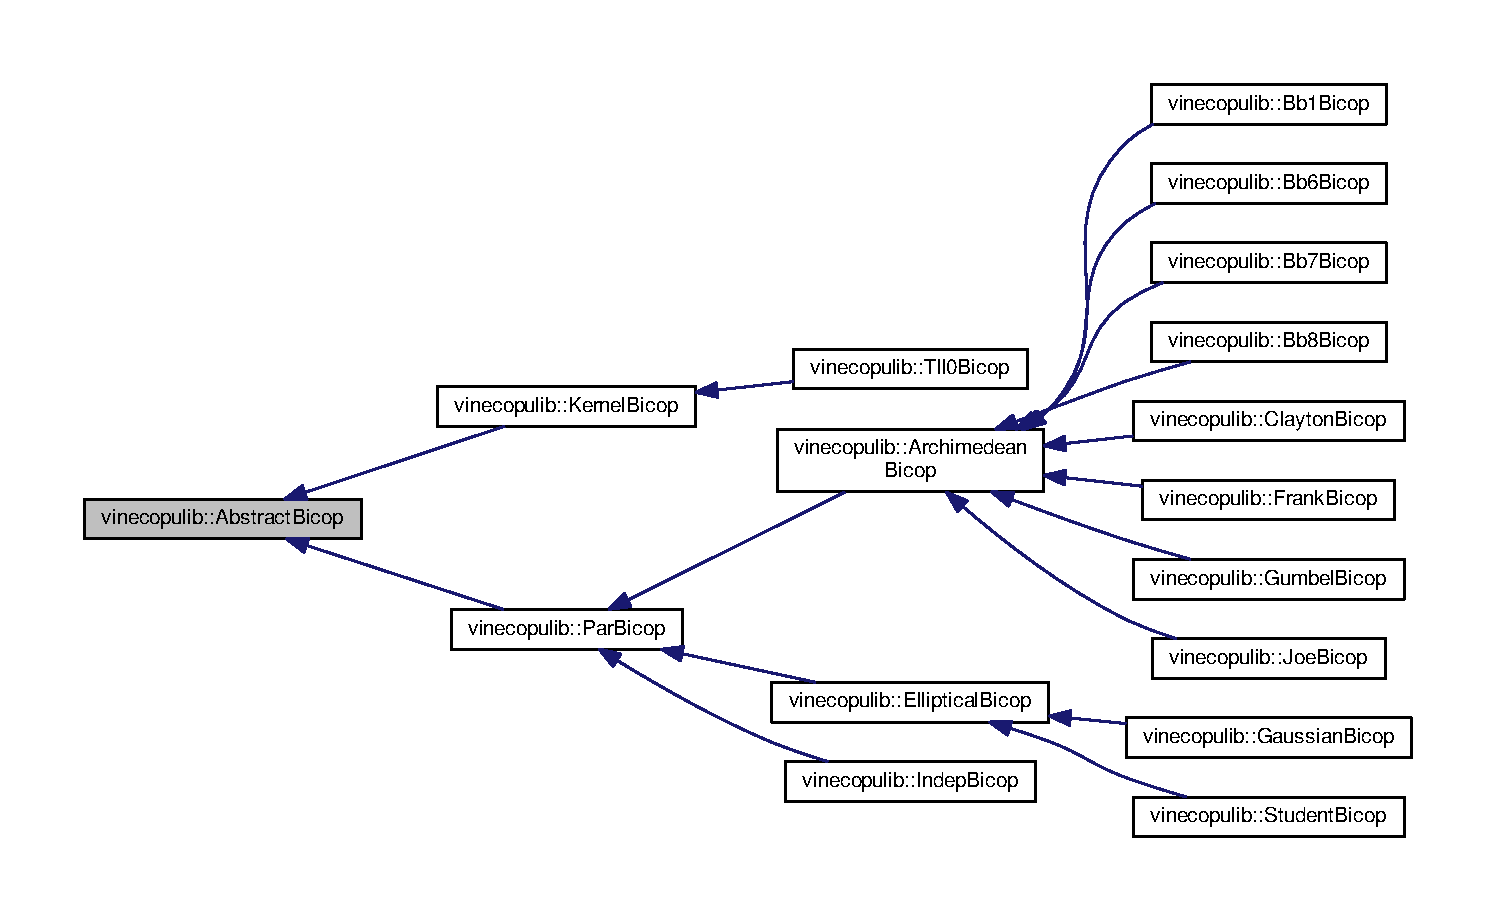
\includegraphics[width=350pt]{classvinecopulib_1_1_abstract_bicop__inherit__graph}
\end{center}
\end{figure}
\subsection*{Protected Member Functions}
\begin{DoxyCompactItemize}
\item 
void \hyperlink{classvinecopulib_1_1_abstract_bicop_a4e62970bb8e533f97f66c280c1a908cf}{flip} ()\hypertarget{classvinecopulib_1_1_abstract_bicop_a4e62970bb8e533f97f66c280c1a908cf}{}\label{classvinecopulib_1_1_abstract_bicop_a4e62970bb8e533f97f66c280c1a908cf}

\begin{DoxyCompactList}\small\item\em Adjust the copula to flipped columns. \end{DoxyCompactList}\item 
virtual void {\bfseries fit} (const Eigen\+::\+Matrix$<$ double, Eigen\+::\+Dynamic, 2 $>$ \&data, std\+::string method, double mult)=0\hypertarget{classvinecopulib_1_1_abstract_bicop_a9cce328189e4637ef86e11fbf4e12a4a}{}\label{classvinecopulib_1_1_abstract_bicop_a9cce328189e4637ef86e11fbf4e12a4a}

\item 
virtual double {\bfseries calculate\+\_\+npars} ()=0\hypertarget{classvinecopulib_1_1_abstract_bicop_af460c2a5a6d2743080b3a883182cd78e}{}\label{classvinecopulib_1_1_abstract_bicop_af460c2a5a6d2743080b3a883182cd78e}

\item 
virtual double {\bfseries parameters\+\_\+to\+\_\+tau} (const Eigen\+::\+Vector\+Xd \&parameters)=0\hypertarget{classvinecopulib_1_1_abstract_bicop_a71ba68887d581483bd51697885dc2d8c}{}\label{classvinecopulib_1_1_abstract_bicop_a71ba68887d581483bd51697885dc2d8c}

\item 
virtual Eigen\+::\+Vector\+Xd {\bfseries pdf} (const Eigen\+::\+Matrix$<$ double, Eigen\+::\+Dynamic, 2 $>$ \&u)=0\hypertarget{classvinecopulib_1_1_abstract_bicop_a4594c3b99a7f2d949a52bf177b1651c3}{}\label{classvinecopulib_1_1_abstract_bicop_a4594c3b99a7f2d949a52bf177b1651c3}

\item 
virtual Eigen\+::\+Vector\+Xd {\bfseries hfunc1} (const Eigen\+::\+Matrix$<$ double, Eigen\+::\+Dynamic, 2 $>$ \&u)=0\hypertarget{classvinecopulib_1_1_abstract_bicop_a2dece0c5a4690e18e8407ea9078522fd}{}\label{classvinecopulib_1_1_abstract_bicop_a2dece0c5a4690e18e8407ea9078522fd}

\item 
virtual Eigen\+::\+Vector\+Xd {\bfseries hfunc2} (const Eigen\+::\+Matrix$<$ double, Eigen\+::\+Dynamic, 2 $>$ \&u)=0\hypertarget{classvinecopulib_1_1_abstract_bicop_a604690344660208cbf7a14aed322d0c6}{}\label{classvinecopulib_1_1_abstract_bicop_a604690344660208cbf7a14aed322d0c6}

\item 
virtual Eigen\+::\+Vector\+Xd {\bfseries hinv1} (const Eigen\+::\+Matrix$<$ double, Eigen\+::\+Dynamic, 2 $>$ \&u)=0\hypertarget{classvinecopulib_1_1_abstract_bicop_a4638c25e1dbb34288b65bcc9f1f6f04e}{}\label{classvinecopulib_1_1_abstract_bicop_a4638c25e1dbb34288b65bcc9f1f6f04e}

\item 
virtual Eigen\+::\+Vector\+Xd {\bfseries hinv2} (const Eigen\+::\+Matrix$<$ double, Eigen\+::\+Dynamic, 2 $>$ \&u)=0\hypertarget{classvinecopulib_1_1_abstract_bicop_a945d782285a9d11a59795e894e8c216b}{}\label{classvinecopulib_1_1_abstract_bicop_a945d782285a9d11a59795e894e8c216b}

\item 
virtual Eigen\+::\+Matrix\+Xd {\bfseries tau\+\_\+to\+\_\+parameters} (const double \&tau)=0\hypertarget{classvinecopulib_1_1_abstract_bicop_a48fc84b668c515745754bfe33ab7cbcf}{}\label{classvinecopulib_1_1_abstract_bicop_a48fc84b668c515745754bfe33ab7cbcf}

\end{DoxyCompactItemize}
{\bf }\par
\begin{DoxyCompactItemize}
\item 
\hyperlink{namespacevinecopulib_a42e95cc06d33896199caab0c11ad44f3}{Bicop\+Family} \hyperlink{classvinecopulib_1_1_abstract_bicop_a61878ff0664fa099f6f6ca4b7ad7833a}{get\+\_\+family} () const 
\item 
std\+::string {\bfseries get\+\_\+family\+\_\+name} () const \hypertarget{classvinecopulib_1_1_abstract_bicop_a294c3d6614fb1d42b4846599292f3197}{}\label{classvinecopulib_1_1_abstract_bicop_a294c3d6614fb1d42b4846599292f3197}

\item 
Eigen\+::\+Matrix\+Xd {\bfseries get\+\_\+parameters} () const \hypertarget{classvinecopulib_1_1_abstract_bicop_a5de117aa32e3e53ef787d517f965f1bc}{}\label{classvinecopulib_1_1_abstract_bicop_a5de117aa32e3e53ef787d517f965f1bc}

\item 
Eigen\+::\+Matrix\+Xd {\bfseries get\+\_\+parameters\+\_\+lower\+\_\+bounds} () const \hypertarget{classvinecopulib_1_1_abstract_bicop_ae7d234b7d647269f21b1904ab17d0a6b}{}\label{classvinecopulib_1_1_abstract_bicop_ae7d234b7d647269f21b1904ab17d0a6b}

\item 
Eigen\+::\+Matrix\+Xd {\bfseries get\+\_\+parameters\+\_\+upper\+\_\+bounds} () const \hypertarget{classvinecopulib_1_1_abstract_bicop_ac772d0c6e28b845a44a721568ac9bbe2}{}\label{classvinecopulib_1_1_abstract_bicop_ac772d0c6e28b845a44a721568ac9bbe2}

\item 
void {\bfseries set\+\_\+parameters} (const Eigen\+::\+Matrix\+Xd \&parameters)\hypertarget{classvinecopulib_1_1_abstract_bicop_a80596978ad8ec752a442f4a41dd0aedc}{}\label{classvinecopulib_1_1_abstract_bicop_a80596978ad8ec752a442f4a41dd0aedc}

\end{DoxyCompactItemize}

{\bf }\par
\begin{DoxyCompactItemize}
\item 
Eigen\+::\+Vector\+Xd \hyperlink{classvinecopulib_1_1_abstract_bicop_a7dc5b05857ece56b7e336e1175387a8e}{hinv1\+\_\+num} (const Eigen\+::\+Matrix$<$ double, Eigen\+::\+Dynamic, 2 $>$ \&u)
\item 
Eigen\+::\+Vector\+Xd {\bfseries hinv2\+\_\+num} (const Eigen\+::\+Matrix$<$ double, Eigen\+::\+Dynamic, 2 $>$ \&u)\hypertarget{classvinecopulib_1_1_abstract_bicop_a8e1077b6f22785f1f4c5fa09b47dae7a}{}\label{classvinecopulib_1_1_abstract_bicop_a8e1077b6f22785f1f4c5fa09b47dae7a}

\end{DoxyCompactItemize}

\subsection*{Static Protected Member Functions}
{\bf }\par
\begin{DoxyCompactItemize}
\item 
static std\+::shared\+\_\+ptr$<$ \hyperlink{classvinecopulib_1_1_abstract_bicop}{Abstract\+Bicop} $>$ \hyperlink{classvinecopulib_1_1_abstract_bicop_afefe048baabaa8cd14e849e66a45c428}{create} (\hyperlink{namespacevinecopulib_a42e95cc06d33896199caab0c11ad44f3}{Bicop\+Family} family=\hyperlink{namespacevinecopulib_a42e95cc06d33896199caab0c11ad44f3af49b022096e968010a7b9bd941805a65}{Bicop\+Family\+::indep}, const Eigen\+::\+Matrix\+Xd \&parameters=Eigen\+::\+Matrix\+Xd())
\end{DoxyCompactItemize}

\subsection*{Protected Attributes}
\begin{DoxyCompactItemize}
\item 
\hyperlink{namespacevinecopulib_a42e95cc06d33896199caab0c11ad44f3}{Bicop\+Family} {\bfseries family\+\_\+}\hypertarget{classvinecopulib_1_1_abstract_bicop_a0b731d28eefd359b1e15951d5e58f093}{}\label{classvinecopulib_1_1_abstract_bicop_a0b731d28eefd359b1e15951d5e58f093}

\item 
Eigen\+::\+Matrix\+Xd {\bfseries parameters\+\_\+}\hypertarget{classvinecopulib_1_1_abstract_bicop_a38f60d7c268c71bf93cfbb4203724478}{}\label{classvinecopulib_1_1_abstract_bicop_a38f60d7c268c71bf93cfbb4203724478}

\item 
Eigen\+::\+Matrix\+Xd {\bfseries parameters\+\_\+lower\+\_\+bounds\+\_\+}\hypertarget{classvinecopulib_1_1_abstract_bicop_ac35229a8c8ab553321f6e4deba646d58}{}\label{classvinecopulib_1_1_abstract_bicop_ac35229a8c8ab553321f6e4deba646d58}

\item 
Eigen\+::\+Matrix\+Xd {\bfseries parameters\+\_\+upper\+\_\+bounds\+\_\+}\hypertarget{classvinecopulib_1_1_abstract_bicop_aab60ca983aac95c3ead7c07db1d227ee}{}\label{classvinecopulib_1_1_abstract_bicop_aab60ca983aac95c3ead7c07db1d227ee}

\end{DoxyCompactItemize}
\subsection*{Friends}
\begin{DoxyCompactItemize}
\item 
class {\bfseries Bicop}\hypertarget{classvinecopulib_1_1_abstract_bicop_af3db9e73153fd7fa7bb69657e7cb949d}{}\label{classvinecopulib_1_1_abstract_bicop_af3db9e73153fd7fa7bb69657e7cb949d}

\item 
double {\bfseries tools\+\_\+optimization\+::mle\+\_\+objective} (const std\+::vector$<$ double $>$ \&x, std\+::vector$<$ double $>$ \&grad, void $\ast$data)\hypertarget{classvinecopulib_1_1_abstract_bicop_ac0e8ae7fffff069ed9476a97d8bfac19}{}\label{classvinecopulib_1_1_abstract_bicop_ac0e8ae7fffff069ed9476a97d8bfac19}

\item 
double {\bfseries tools\+\_\+optimization\+::pmle\+\_\+objective} (const std\+::vector$<$ double $>$ \&x, std\+::vector$<$ double $>$ \&grad, void $\ast$data)\hypertarget{classvinecopulib_1_1_abstract_bicop_ae671e9f66df15a190329d53c802f70ef}{}\label{classvinecopulib_1_1_abstract_bicop_ae671e9f66df15a190329d53c802f70ef}

\end{DoxyCompactItemize}


\subsection{Detailed Description}
An abstract class for bivariate copula families. 

This class is used in the implementation underlying the \hyperlink{classvinecopulib_1_1_bicop}{Bicop} class. Users should not use \hyperlink{classvinecopulib_1_1_abstract_bicop}{Abstract\+Bicop} or derived classes directly, but always work with the \hyperlink{classvinecopulib_1_1_bicop}{Bicop} interface. 

\subsection{Member Function Documentation}
\index{vinecopulib\+::\+Abstract\+Bicop@{vinecopulib\+::\+Abstract\+Bicop}!create@{create}}
\index{create@{create}!vinecopulib\+::\+Abstract\+Bicop@{vinecopulib\+::\+Abstract\+Bicop}}
\subsubsection[{\texorpdfstring{create(\+Bicop\+Family family=\+Bicop\+Family\+::indep, const Eigen\+::\+Matrix\+Xd \&parameters=\+Eigen\+::\+Matrix\+Xd())}{create(BicopFamily family=BicopFamily::indep, const Eigen::MatrixXd &parameters=Eigen::MatrixXd())}}]{\setlength{\rightskip}{0pt plus 5cm}{\bf Bicop\+Ptr} vinecopulib\+::\+Abstract\+Bicop\+::create (
\begin{DoxyParamCaption}
\item[{{\bf Bicop\+Family}}]{family = {\ttfamily {\bf Bicop\+Family\+::indep}}, }
\item[{const Eigen\+::\+Matrix\+Xd \&}]{parameters = {\ttfamily Eigen\+:\+:MatrixXd()}}
\end{DoxyParamCaption}
)\hspace{0.3cm}{\ttfamily [static]}, {\ttfamily [protected]}}\hypertarget{classvinecopulib_1_1_abstract_bicop_afefe048baabaa8cd14e849e66a45c428}{}\label{classvinecopulib_1_1_abstract_bicop_afefe048baabaa8cd14e849e66a45c428}
Create a bivariate copula using the default contructor


\begin{DoxyParams}{Parameters}
{\em family} & the copula family. \\
\hline
{\em parameters} & the copula parameters (optional, must be compatible with family). \\
\hline
\end{DoxyParams}
\begin{DoxyReturn}{Returns}
A pointer to an object that inherits from \hyperlink{classvinecopulib_1_1_abstract_bicop}{Abstract\+Bicop}. 
\end{DoxyReturn}
\index{vinecopulib\+::\+Abstract\+Bicop@{vinecopulib\+::\+Abstract\+Bicop}!get\+\_\+family@{get\+\_\+family}}
\index{get\+\_\+family@{get\+\_\+family}!vinecopulib\+::\+Abstract\+Bicop@{vinecopulib\+::\+Abstract\+Bicop}}
\subsubsection[{\texorpdfstring{get\+\_\+family() const }{get_family() const }}]{\setlength{\rightskip}{0pt plus 5cm}{\bf Bicop\+Family} vinecopulib\+::\+Abstract\+Bicop\+::get\+\_\+family (
\begin{DoxyParamCaption}
{}
\end{DoxyParamCaption}
) const\hspace{0.3cm}{\ttfamily [protected]}}\hypertarget{classvinecopulib_1_1_abstract_bicop_a61878ff0664fa099f6f6ca4b7ad7833a}{}\label{classvinecopulib_1_1_abstract_bicop_a61878ff0664fa099f6f6ca4b7ad7833a}
Getters and setters. \index{vinecopulib\+::\+Abstract\+Bicop@{vinecopulib\+::\+Abstract\+Bicop}!hinv1\+\_\+num@{hinv1\+\_\+num}}
\index{hinv1\+\_\+num@{hinv1\+\_\+num}!vinecopulib\+::\+Abstract\+Bicop@{vinecopulib\+::\+Abstract\+Bicop}}
\subsubsection[{\texorpdfstring{hinv1\+\_\+num(const Eigen\+::\+Matrix$<$ double, Eigen\+::\+Dynamic, 2 $>$ \&u)}{hinv1_num(const Eigen::Matrix< double, Eigen::Dynamic, 2 > &u)}}]{\setlength{\rightskip}{0pt plus 5cm}Eigen\+::\+Vector\+Xd vinecopulib\+::\+Abstract\+Bicop\+::hinv1\+\_\+num (
\begin{DoxyParamCaption}
\item[{const Eigen\+::\+Matrix$<$ double, Eigen\+::\+Dynamic, 2 $>$ \&}]{u}
\end{DoxyParamCaption}
)\hspace{0.3cm}{\ttfamily [protected]}}\hypertarget{classvinecopulib_1_1_abstract_bicop_a7dc5b05857ece56b7e336e1175387a8e}{}\label{classvinecopulib_1_1_abstract_bicop_a7dc5b05857ece56b7e336e1175387a8e}
Numerical inversion of h-\/functions

These are generic functions to invert the hfunctions numerically. They can be used in derived classes to define {\ttfamily hinv1} and {\ttfamily hinv2}.


\begin{DoxyParams}{Parameters}
{\em u} & $m \times 2$ matrix of evaluation points. \\
\hline
\end{DoxyParams}
\begin{DoxyReturn}{Returns}
The numerical inverse of h-\/functions. 
\end{DoxyReturn}


The documentation for this class was generated from the following files\+:\begin{DoxyCompactItemize}
\item 
/home/n5/dev/cpp/vinecopulib/include/bicop/abstract.\+hpp\item 
/home/n5/dev/cpp/vinecopulib/src/bicop/abstract.\+cpp\end{DoxyCompactItemize}

\hypertarget{classvinecopulib_1_1_archimedean_bicop}{}\section{vinecopulib\+:\+:Archimedean\+Bicop Class Reference}
\label{classvinecopulib_1_1_archimedean_bicop}\index{vinecopulib\+::\+Archimedean\+Bicop@{vinecopulib\+::\+Archimedean\+Bicop}}


An abstract class for Archimedean copula families.  




{\ttfamily \#include $<$archimedean.\+hpp$>$}



Inheritance diagram for vinecopulib\+:\+:Archimedean\+Bicop\+:
\nopagebreak
\begin{figure}[H]
\begin{center}
\leavevmode
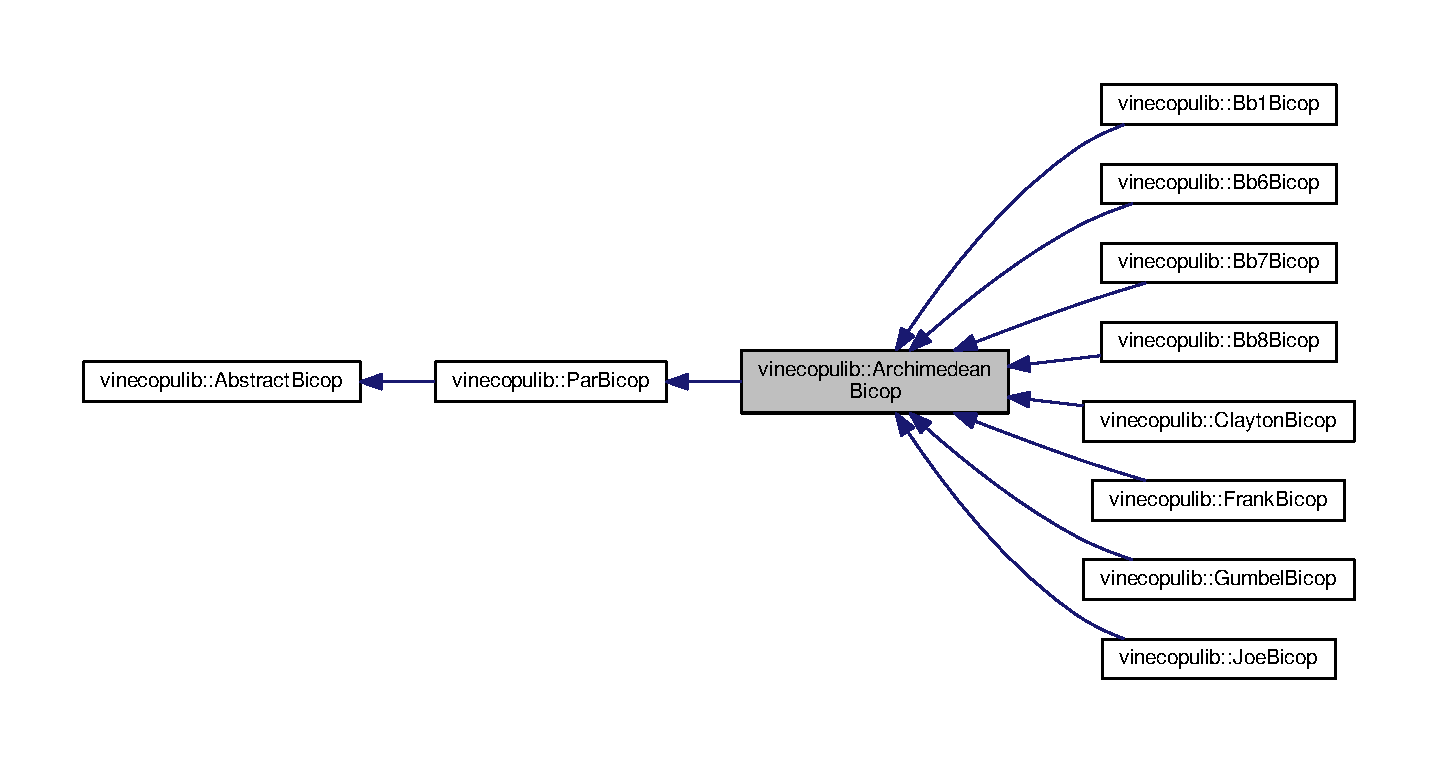
\includegraphics[width=350pt]{classvinecopulib_1_1_archimedean_bicop__inherit__graph}
\end{center}
\end{figure}


Collaboration diagram for vinecopulib\+:\+:Archimedean\+Bicop\+:
\nopagebreak
\begin{figure}[H]
\begin{center}
\leavevmode
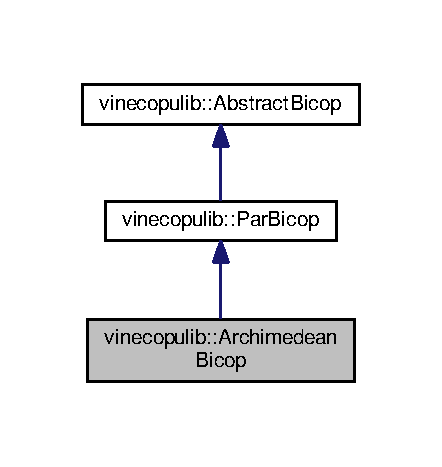
\includegraphics[width=213pt]{classvinecopulib_1_1_archimedean_bicop__coll__graph}
\end{center}
\end{figure}
\subsection*{Additional Inherited Members}


\subsection{Detailed Description}
An abstract class for Archimedean copula families. 

This class is used in the implementation underlying the \hyperlink{classvinecopulib_1_1_bicop}{Bicop} class. Users should not use \hyperlink{classvinecopulib_1_1_abstract_bicop}{Abstract\+Bicop} or derived classes directly, but always work with the \hyperlink{classvinecopulib_1_1_bicop}{Bicop} interface.

Joe, Harry. Dependence modeling with copulas. C\+RC Press, 2014. 

The documentation for this class was generated from the following files\+:\begin{DoxyCompactItemize}
\item 
/home/n5/dev/cpp/vinecopulib/include/bicop/archimedean.\+hpp\item 
/home/n5/dev/cpp/vinecopulib/src/bicop/archimedean.\+cpp\end{DoxyCompactItemize}

\hypertarget{classvinecopulib_1_1_bb1_bicop}{}\section{vinecopulib\+:\+:Bb1\+Bicop Class Reference}
\label{classvinecopulib_1_1_bb1_bicop}\index{vinecopulib\+::\+Bb1\+Bicop@{vinecopulib\+::\+Bb1\+Bicop}}


The B\+B1 copula.  




{\ttfamily \#include $<$bb1.\+hpp$>$}



Inheritance diagram for vinecopulib\+:\+:Bb1\+Bicop\+:
\nopagebreak
\begin{figure}[H]
\begin{center}
\leavevmode
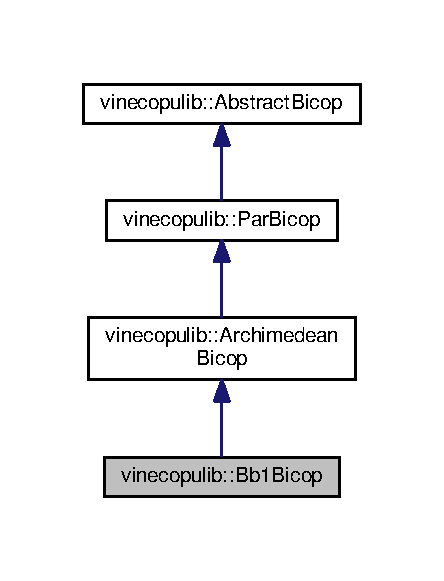
\includegraphics[width=213pt]{classvinecopulib_1_1_bb1_bicop__inherit__graph}
\end{center}
\end{figure}


Collaboration diagram for vinecopulib\+:\+:Bb1\+Bicop\+:
\nopagebreak
\begin{figure}[H]
\begin{center}
\leavevmode
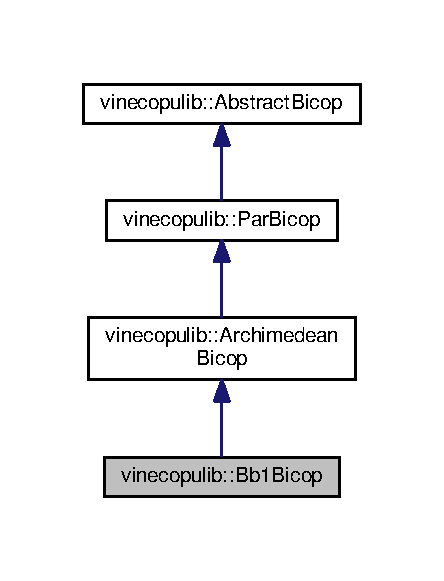
\includegraphics[width=213pt]{classvinecopulib_1_1_bb1_bicop__coll__graph}
\end{center}
\end{figure}
\subsection*{Additional Inherited Members}


\subsection{Detailed Description}
The B\+B1 copula. 

This class is used in the implementation underlying the \hyperlink{classvinecopulib_1_1_bicop}{Bicop} class. Users should not use \hyperlink{classvinecopulib_1_1_abstract_bicop}{Abstract\+Bicop} or derived classes directly, but always work with the \hyperlink{classvinecopulib_1_1_bicop}{Bicop} interface.

Joe, Harry. Dependence modeling with copulas. C\+RC Press, 2014. 

The documentation for this class was generated from the following files\+:\begin{DoxyCompactItemize}
\item 
/home/n5/dev/cpp/vinecopulib/include/bicop/bb1.\+hpp\item 
/home/n5/dev/cpp/vinecopulib/src/bicop/bb1.\+cpp\end{DoxyCompactItemize}

\hypertarget{classvinecopulib_1_1_bb6_bicop}{\section{vinecopulib\+:\+:Bb6\+Bicop Class Reference}
\label{classvinecopulib_1_1_bb6_bicop}\index{vinecopulib\+::\+Bb6\+Bicop@{vinecopulib\+::\+Bb6\+Bicop}}
}


The B\+B6 copula.  




{\ttfamily \#include $<$bb6.\+hpp$>$}



Inheritance diagram for vinecopulib\+:\+:Bb6\+Bicop\+:\nopagebreak
\begin{figure}[H]
\begin{center}
\leavevmode
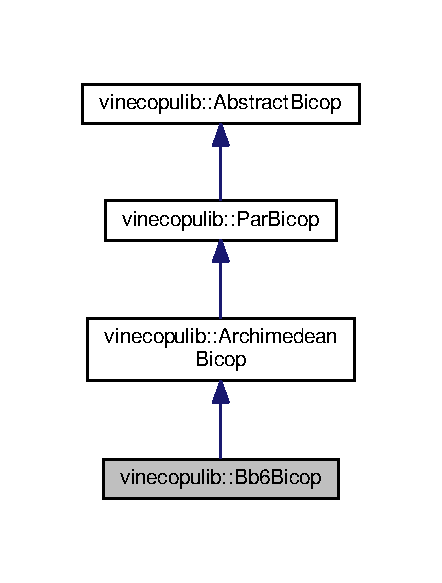
\includegraphics[width=212pt]{classvinecopulib_1_1_bb6_bicop__inherit__graph}
\end{center}
\end{figure}


Collaboration diagram for vinecopulib\+:\+:Bb6\+Bicop\+:\nopagebreak
\begin{figure}[H]
\begin{center}
\leavevmode
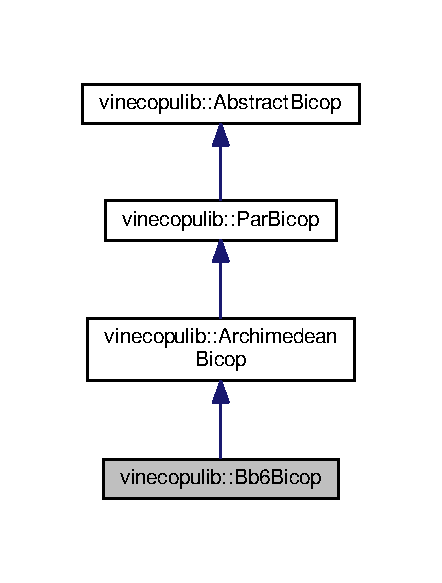
\includegraphics[width=212pt]{classvinecopulib_1_1_bb6_bicop__coll__graph}
\end{center}
\end{figure}
\subsection*{Additional Inherited Members}


\subsection{Detailed Description}
The B\+B6 copula. 

This class is used in the implementation underlying the \hyperlink{classvinecopulib_1_1_bicop}{Bicop} class. Users should not use \hyperlink{classvinecopulib_1_1_abstract_bicop}{Abstract\+Bicop} or derived classes directly, but always work with the \hyperlink{classvinecopulib_1_1_bicop}{Bicop} interface.

Joe, Harry. Dependence modeling with copulas. C\+R\+C Press, 2014. 

The documentation for this class was generated from the following files\+:\begin{DoxyCompactItemize}
\item 
vinecopulib/include/vinecopulib/bicop/bb6.\+hpp\item 
vinecopulib/src/bicop/bb6.\+cpp\end{DoxyCompactItemize}

\hypertarget{classvinecopulib_1_1_bb7_bicop}{}\section{vinecopulib\+:\+:Bb7\+Bicop Class Reference}
\label{classvinecopulib_1_1_bb7_bicop}\index{vinecopulib\+::\+Bb7\+Bicop@{vinecopulib\+::\+Bb7\+Bicop}}


The B\+B7 copula.  




{\ttfamily \#include $<$bb7.\+hpp$>$}



Inheritance diagram for vinecopulib\+:\+:Bb7\+Bicop\+:
\nopagebreak
\begin{figure}[H]
\begin{center}
\leavevmode
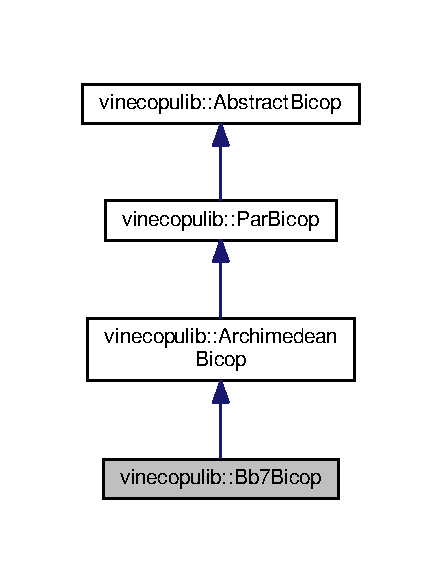
\includegraphics[width=213pt]{classvinecopulib_1_1_bb7_bicop__inherit__graph}
\end{center}
\end{figure}


Collaboration diagram for vinecopulib\+:\+:Bb7\+Bicop\+:
\nopagebreak
\begin{figure}[H]
\begin{center}
\leavevmode
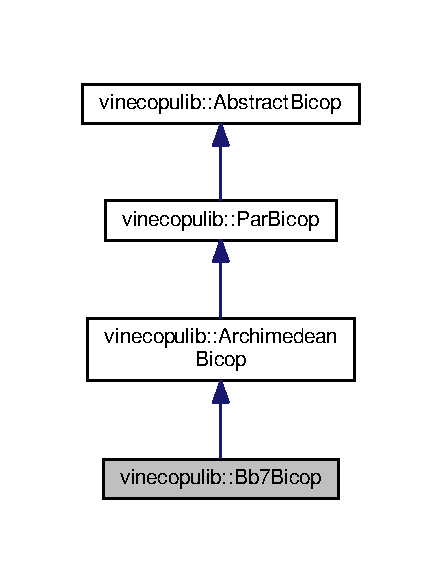
\includegraphics[width=213pt]{classvinecopulib_1_1_bb7_bicop__coll__graph}
\end{center}
\end{figure}
\subsection*{Additional Inherited Members}


\subsection{Detailed Description}
The B\+B7 copula. 

This class is used in the implementation underlying the \hyperlink{classvinecopulib_1_1_bicop}{Bicop} class. Users should not use \hyperlink{classvinecopulib_1_1_abstract_bicop}{Abstract\+Bicop} or derived classes directly, but always work with the \hyperlink{classvinecopulib_1_1_bicop}{Bicop} interface.

Joe, Harry. Dependence modeling with copulas. C\+RC Press, 2014. 

The documentation for this class was generated from the following files\+:\begin{DoxyCompactItemize}
\item 
/home/n5/dev/cpp/vinecopulib/include/bicop/bb7.\+hpp\item 
/home/n5/dev/cpp/vinecopulib/src/bicop/bb7.\+cpp\end{DoxyCompactItemize}

\hypertarget{classvinecopulib_1_1_bb8_bicop}{}\section{vinecopulib\+:\+:Bb8\+Bicop Class Reference}
\label{classvinecopulib_1_1_bb8_bicop}\index{vinecopulib\+::\+Bb8\+Bicop@{vinecopulib\+::\+Bb8\+Bicop}}


Inheritance diagram for vinecopulib\+:\+:Bb8\+Bicop\+:\nopagebreak
\begin{figure}[H]
\begin{center}
\leavevmode
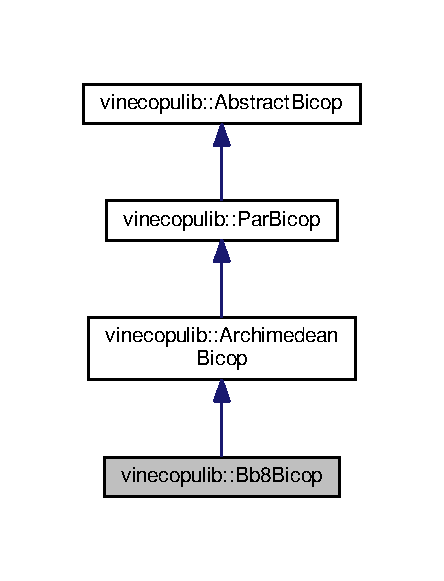
\includegraphics[width=208pt]{classvinecopulib_1_1_bb8_bicop__inherit__graph}
\end{center}
\end{figure}


Collaboration diagram for vinecopulib\+:\+:Bb8\+Bicop\+:\nopagebreak
\begin{figure}[H]
\begin{center}
\leavevmode
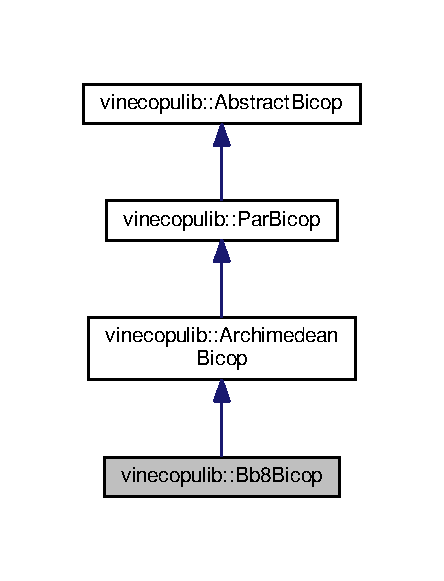
\includegraphics[width=208pt]{classvinecopulib_1_1_bb8_bicop__coll__graph}
\end{center}
\end{figure}
\subsection*{Additional Inherited Members}


The documentation for this class was generated from the following files\+:\begin{DoxyCompactItemize}
\item 
/home/n5/dev/cpp/vinecopulib/include/bicop\+\_\+bb8.\+hpp\item 
/home/n5/dev/cpp/vinecopulib/src/bicop\+\_\+bb8.\+cpp\end{DoxyCompactItemize}

\hypertarget{classvinecopulib_1_1_bicop}{\section{vinecopulib\+:\+:Bicop Class Reference}
\label{classvinecopulib_1_1_bicop}\index{vinecopulib\+::\+Bicop@{vinecopulib\+::\+Bicop}}
}


A class for bivariate copula models.  




{\ttfamily \#include $<$class.\+hpp$>$}

\subsection*{Public Member Functions}
\begin{DoxyCompactItemize}
\item 
\hypertarget{classvinecopulib_1_1_bicop_acfa522fb0bea4aca8fade87c18bcf921}{\hyperlink{classvinecopulib_1_1_bicop_acfa522fb0bea4aca8fade87c18bcf921}{Bicop} ()}\label{classvinecopulib_1_1_bicop_acfa522fb0bea4aca8fade87c18bcf921}

\begin{DoxyCompactList}\small\item\em creates the independence copula. \end{DoxyCompactList}\item 
\hyperlink{classvinecopulib_1_1_bicop_ab27f789e001e30f2fed7f9ecefdeffb0}{Bicop} (\hyperlink{namespacevinecopulib_a42e95cc06d33896199caab0c11ad44f3}{Bicop\+Family} family, int rotation=0, const Eigen\+::\+Matrix\+Xd \&parameters=Eigen\+::\+Matrix\+Xd())
\item 
\hyperlink{classvinecopulib_1_1_bicop_afc8b465d9e02a3df1c25f7c1e7ac9240}{Bicop} (Eigen\+::\+Matrix$<$ double, Eigen\+::\+Dynamic, 2 $>$ data, \hyperlink{classvinecopulib_1_1_fit_controls_bicop}{Fit\+Controls\+Bicop} controls=\hyperlink{classvinecopulib_1_1_fit_controls_bicop}{Fit\+Controls\+Bicop}())
\item 
Eigen\+::\+Vector\+Xd \hyperlink{classvinecopulib_1_1_bicop_a83dc7214e4bb1bfe59285ca05407d646}{pdf} (const Eigen\+::\+Matrix$<$ double, Eigen\+::\+Dynamic, 2 $>$ \&u)
\item 
Eigen\+::\+Vector\+Xd \hyperlink{classvinecopulib_1_1_bicop_a153d7e766388066eda14577c5a6332cc}{cdf} (const Eigen\+::\+Matrix$<$ double, Eigen\+::\+Dynamic, 2 $>$ \&u)
\item 
Eigen\+::\+Vector\+Xd \hyperlink{classvinecopulib_1_1_bicop_a130fda62cd61c7acdef5db75fffdd89e}{hfunc1} (const Eigen\+::\+Matrix$<$ double, Eigen\+::\+Dynamic, 2 $>$ \&u)
\item 
Eigen\+::\+Vector\+Xd \hyperlink{classvinecopulib_1_1_bicop_a4c9b50f99797ec374f5057cc54db2bd8}{hfunc2} (const Eigen\+::\+Matrix$<$ double, Eigen\+::\+Dynamic, 2 $>$ \&u)
\item 
Eigen\+::\+Vector\+Xd \hyperlink{classvinecopulib_1_1_bicop_a3cc8b161ec6efdb3b34d2efa9185bf44}{hinv1} (const Eigen\+::\+Matrix$<$ double, Eigen\+::\+Dynamic, 2 $>$ \&u)
\item 
Eigen\+::\+Vector\+Xd \hyperlink{classvinecopulib_1_1_bicop_a3e33ec227b6b7182e327399201cad382}{hinv2} (const Eigen\+::\+Matrix$<$ double, Eigen\+::\+Dynamic, 2 $>$ \&u)
\item 
Eigen\+::\+Matrix$<$ double, \\*
Eigen\+::\+Dynamic, 2 $>$ \hyperlink{classvinecopulib_1_1_bicop_aeb87bea4283dacfa5e609356c020f85d}{simulate} (const int \&n)
\item 
void \hyperlink{classvinecopulib_1_1_bicop_a2d509a8b404a73ef17f04a0678e90a71}{fit} (const Eigen\+::\+Matrix$<$ double, Eigen\+::\+Dynamic, 2 $>$ \&data, \hyperlink{classvinecopulib_1_1_fit_controls_bicop}{Fit\+Controls\+Bicop} controls=\hyperlink{classvinecopulib_1_1_fit_controls_bicop}{Fit\+Controls\+Bicop}())
\item 
void \hyperlink{classvinecopulib_1_1_bicop_af20af5c3ba6565628987b4784e9ac348}{select} (Eigen\+::\+Matrix$<$ double, Eigen\+::\+Dynamic, 2 $>$ data, \hyperlink{classvinecopulib_1_1_fit_controls_bicop}{Fit\+Controls\+Bicop} controls=\hyperlink{classvinecopulib_1_1_fit_controls_bicop}{Fit\+Controls\+Bicop}())
\item 
double \hyperlink{classvinecopulib_1_1_bicop_ae8bcc0c3265cc86565333a0cfd3d619d}{loglik} (const Eigen\+::\+Matrix$<$ double, Eigen\+::\+Dynamic, 2 $>$ \&u)
\item 
double \hyperlink{classvinecopulib_1_1_bicop_a9287fec95519fea64a2ae80f5888c709}{aic} (const Eigen\+::\+Matrix$<$ double, Eigen\+::\+Dynamic, 2 $>$ \&u)
\item 
double \hyperlink{classvinecopulib_1_1_bicop_ac1f480d13b3464260c2dd6aa88b2e130}{bic} (const Eigen\+::\+Matrix$<$ double, Eigen\+::\+Dynamic, 2 $>$ \&u)
\item 
double \hyperlink{classvinecopulib_1_1_bicop_a9f3b3b83c54a9e1d809fdee058f3eb11}{calculate\+\_\+npars} ()
\item 
double \hyperlink{classvinecopulib_1_1_bicop_aa25436353dee76e4368fb941a7efa257}{parameters\+\_\+to\+\_\+tau} (const Eigen\+::\+Vector\+Xd \&parameters)
\item 
Eigen\+::\+Matrix\+Xd \hyperlink{classvinecopulib_1_1_bicop_a5809ddc9884f6fb66fe53289be348913}{tau\+\_\+to\+\_\+parameters} (const double \&tau)
\end{DoxyCompactItemize}
\begin{Indent}{\bf Getters and setters}\par
\begin{DoxyCompactItemize}
\item 
\hypertarget{classvinecopulib_1_1_bicop_a68ab3556ee3bb3d02814fd978573bf3b}{\hyperlink{namespacevinecopulib_a42e95cc06d33896199caab0c11ad44f3}{Bicop\+Family} {\bfseries get\+\_\+family} () const }\label{classvinecopulib_1_1_bicop_a68ab3556ee3bb3d02814fd978573bf3b}

\item 
\hypertarget{classvinecopulib_1_1_bicop_a4d4fbc0fdca17564c23f4814d5d2fbe7}{std\+::string {\bfseries get\+\_\+family\+\_\+name} () const }\label{classvinecopulib_1_1_bicop_a4d4fbc0fdca17564c23f4814d5d2fbe7}

\item 
\hypertarget{classvinecopulib_1_1_bicop_ab8e52577a50fbfc57277f9240d8eac03}{int {\bfseries get\+\_\+rotation} () const }\label{classvinecopulib_1_1_bicop_ab8e52577a50fbfc57277f9240d8eac03}

\item 
\hypertarget{classvinecopulib_1_1_bicop_a93ab0dd89826e50b209ea3760f251f2f}{Eigen\+::\+Matrix\+Xd {\bfseries get\+\_\+parameters} () const }\label{classvinecopulib_1_1_bicop_a93ab0dd89826e50b209ea3760f251f2f}

\item 
void \hyperlink{classvinecopulib_1_1_bicop_a4e359624560a089273b25dc74879bd16}{set\+\_\+rotation} (int rotation)
\item 
void \hyperlink{classvinecopulib_1_1_bicop_ac8d1d4266b0fd7e2f971d0149f881ef9}{set\+\_\+parameters} (const Eigen\+::\+Matrix\+Xd \&parameters)
\end{DoxyCompactItemize}
\end{Indent}
\begin{Indent}{\bf Utilities}\par
{\em adjust's the copula model to a change in the variable order. }\begin{DoxyCompactItemize}
\item 
\hypertarget{classvinecopulib_1_1_bicop_a94b889d56f478dbeb156be4e31af5de5}{std\+::string \hyperlink{classvinecopulib_1_1_bicop_a94b889d56f478dbeb156be4e31af5de5}{str} ()}\label{classvinecopulib_1_1_bicop_a94b889d56f478dbeb156be4e31af5de5}

\begin{DoxyCompactList}\small\item\em summarizes the model into a string (can be used for printing). \end{DoxyCompactList}\item 
\hypertarget{classvinecopulib_1_1_bicop_a59b7087b3857350df25ff684ab96f377}{void {\bfseries flip} ()}\label{classvinecopulib_1_1_bicop_a59b7087b3857350df25ff684ab96f377}

\end{DoxyCompactItemize}
\end{Indent}


\subsection{Detailed Description}
A class for bivariate copula models. 

The copula model is fully characterized by the family, rotation, and parameters. 

\subsection{Constructor \& Destructor Documentation}
\hypertarget{classvinecopulib_1_1_bicop_ab27f789e001e30f2fed7f9ecefdeffb0}{\index{vinecopulib\+::\+Bicop@{vinecopulib\+::\+Bicop}!Bicop@{Bicop}}
\index{Bicop@{Bicop}!vinecopulib\+::\+Bicop@{vinecopulib\+::\+Bicop}}
\subsubsection[{Bicop}]{\setlength{\rightskip}{0pt plus 5cm}vinecopulib\+::\+Bicop\+::\+Bicop (
\begin{DoxyParamCaption}
\item[{{\bf Bicop\+Family}}]{family, }
\item[{int}]{rotation = {\ttfamily 0}, }
\item[{const Eigen\+::\+Matrix\+Xd \&}]{parameters = {\ttfamily Eigen\+:\+:MatrixXd()}}
\end{DoxyParamCaption}
)}}\label{classvinecopulib_1_1_bicop_ab27f789e001e30f2fed7f9ecefdeffb0}
creates a specific bivariate copula model. 
\begin{DoxyParams}{Parameters}
{\em family} & the copula family. \\
\hline
{\em rotation} & the rotation of the copula; one of 0, 90, 180, or 270 (for Independence, Gaussian, Student, Frank, and nonparametric families, only 0 is allowed). \\
\hline
{\em parameters} & the copula parameters. \\
\hline
\end{DoxyParams}
\hypertarget{classvinecopulib_1_1_bicop_afc8b465d9e02a3df1c25f7c1e7ac9240}{\index{vinecopulib\+::\+Bicop@{vinecopulib\+::\+Bicop}!Bicop@{Bicop}}
\index{Bicop@{Bicop}!vinecopulib\+::\+Bicop@{vinecopulib\+::\+Bicop}}
\subsubsection[{Bicop}]{\setlength{\rightskip}{0pt plus 5cm}vinecopulib\+::\+Bicop\+::\+Bicop (
\begin{DoxyParamCaption}
\item[{Eigen\+::\+Matrix$<$ double, Eigen\+::\+Dynamic, 2 $>$}]{data, }
\item[{{\bf Fit\+Controls\+Bicop}}]{controls = {\ttfamily {\bf Fit\+Controls\+Bicop}()}}
\end{DoxyParamCaption}
)}}\label{classvinecopulib_1_1_bicop_afc8b465d9e02a3df1c25f7c1e7ac9240}
equivalent to {\ttfamily \hyperlink{classvinecopulib_1_1_bicop}{Bicop} cop; cop.\+select(data, controls)}. 
\begin{DoxyParams}{Parameters}
{\em data} & see \hyperlink{classvinecopulib_1_1_bicop_af20af5c3ba6565628987b4784e9ac348}{select()}. \\
\hline
{\em controls} & see \hyperlink{classvinecopulib_1_1_bicop_af20af5c3ba6565628987b4784e9ac348}{select()}. \\
\hline
\end{DoxyParams}


\subsection{Member Function Documentation}
\hypertarget{classvinecopulib_1_1_bicop_a9287fec95519fea64a2ae80f5888c709}{\index{vinecopulib\+::\+Bicop@{vinecopulib\+::\+Bicop}!aic@{aic}}
\index{aic@{aic}!vinecopulib\+::\+Bicop@{vinecopulib\+::\+Bicop}}
\subsubsection[{aic}]{\setlength{\rightskip}{0pt plus 5cm}double vinecopulib\+::\+Bicop\+::aic (
\begin{DoxyParamCaption}
\item[{const Eigen\+::\+Matrix$<$ double, Eigen\+::\+Dynamic, 2 $>$ \&}]{u}
\end{DoxyParamCaption}
)}}\label{classvinecopulib_1_1_bicop_a9287fec95519fea64a2ae80f5888c709}
calculates the Akaike information criterion (A\+I\+C).

The A\+I\+C is defined as \[ \mathrm{AIC} = -2\, \mathrm{loglik} + 2 p, \] where $ \mathrm{loglik} $ is the log-\/liklihood and $ p $ is the (effective) number of parameters of the model, see \hyperlink{classvinecopulib_1_1_bicop_ae8bcc0c3265cc86565333a0cfd3d619d}{loglik()} and \hyperlink{classvinecopulib_1_1_bicop_a9f3b3b83c54a9e1d809fdee058f3eb11}{calculate\+\_\+npars()}. The A\+I\+C is a consistent model selection criterion for nonparametric models.


\begin{DoxyParams}{Parameters}
{\em u} & $n \times 2$ matrix of observations. \\
\hline
\end{DoxyParams}
\hypertarget{classvinecopulib_1_1_bicop_ac1f480d13b3464260c2dd6aa88b2e130}{\index{vinecopulib\+::\+Bicop@{vinecopulib\+::\+Bicop}!bic@{bic}}
\index{bic@{bic}!vinecopulib\+::\+Bicop@{vinecopulib\+::\+Bicop}}
\subsubsection[{bic}]{\setlength{\rightskip}{0pt plus 5cm}double vinecopulib\+::\+Bicop\+::bic (
\begin{DoxyParamCaption}
\item[{const Eigen\+::\+Matrix$<$ double, Eigen\+::\+Dynamic, 2 $>$ \&}]{u}
\end{DoxyParamCaption}
)}}\label{classvinecopulib_1_1_bicop_ac1f480d13b3464260c2dd6aa88b2e130}
calculates the Bayesian information criterion (B\+I\+C).

The B\+I\+C is defined as \[ \mathrm{BIC} = -2\, \mathrm{loglik} + \ln(n) p, \] where $ \mathrm{loglik} $ is the log-\/liklihood and $ p $ is the (effective) number of parameters of the model, see \hyperlink{classvinecopulib_1_1_bicop_ae8bcc0c3265cc86565333a0cfd3d619d}{loglik()} and \hyperlink{classvinecopulib_1_1_bicop_a9f3b3b83c54a9e1d809fdee058f3eb11}{calculate\+\_\+npars()}. The B\+I\+C is a consistent model selection criterion for nonparametric models.


\begin{DoxyParams}{Parameters}
{\em u} & $n \times 2$ matrix of observations. \\
\hline
\end{DoxyParams}
\hypertarget{classvinecopulib_1_1_bicop_a9f3b3b83c54a9e1d809fdee058f3eb11}{\index{vinecopulib\+::\+Bicop@{vinecopulib\+::\+Bicop}!calculate\+\_\+npars@{calculate\+\_\+npars}}
\index{calculate\+\_\+npars@{calculate\+\_\+npars}!vinecopulib\+::\+Bicop@{vinecopulib\+::\+Bicop}}
\subsubsection[{calculate\+\_\+npars}]{\setlength{\rightskip}{0pt plus 5cm}double vinecopulib\+::\+Bicop\+::calculate\+\_\+npars (
\begin{DoxyParamCaption}
{}
\end{DoxyParamCaption}
)}}\label{classvinecopulib_1_1_bicop_a9f3b3b83c54a9e1d809fdee058f3eb11}
calculates the effective number of parameters.

Returns the actual number of parameters for parameteric families. For nonparametric families, there is a conceptually similar definition in the sense that it can be used in the calculation of fit statistics. \hypertarget{classvinecopulib_1_1_bicop_a153d7e766388066eda14577c5a6332cc}{\index{vinecopulib\+::\+Bicop@{vinecopulib\+::\+Bicop}!cdf@{cdf}}
\index{cdf@{cdf}!vinecopulib\+::\+Bicop@{vinecopulib\+::\+Bicop}}
\subsubsection[{cdf}]{\setlength{\rightskip}{0pt plus 5cm}Eigen\+::\+Vector\+Xd vinecopulib\+::\+Bicop\+::cdf (
\begin{DoxyParamCaption}
\item[{const Eigen\+::\+Matrix$<$ double, Eigen\+::\+Dynamic, 2 $>$ \&}]{u}
\end{DoxyParamCaption}
)}}\label{classvinecopulib_1_1_bicop_a153d7e766388066eda14577c5a6332cc}
evaluates the copula distribution.


\begin{DoxyParams}{Parameters}
{\em u} & $n \times 2$ matrix of evaluation points. \\
\hline
\end{DoxyParams}
\begin{DoxyReturn}{Returns}
The copula distribution evaluated at {\ttfamily u}. 
\end{DoxyReturn}
\hypertarget{classvinecopulib_1_1_bicop_a2d509a8b404a73ef17f04a0678e90a71}{\index{vinecopulib\+::\+Bicop@{vinecopulib\+::\+Bicop}!fit@{fit}}
\index{fit@{fit}!vinecopulib\+::\+Bicop@{vinecopulib\+::\+Bicop}}
\subsubsection[{fit}]{\setlength{\rightskip}{0pt plus 5cm}void vinecopulib\+::\+Bicop\+::fit (
\begin{DoxyParamCaption}
\item[{const Eigen\+::\+Matrix$<$ double, Eigen\+::\+Dynamic, 2 $>$ \&}]{data, }
\item[{{\bf Fit\+Controls\+Bicop}}]{controls = {\ttfamily {\bf Fit\+Controls\+Bicop}()}}
\end{DoxyParamCaption}
)}}\label{classvinecopulib_1_1_bicop_a2d509a8b404a73ef17f04a0678e90a71}
fits a bivariate copula (with fixed family) to data.

For parametric models, two different methods are available. {\ttfamily \char`\"{}mle\char`\"{}} fits the parameters by maximum-\/likelihood. {\ttfamily \char`\"{}itau\char`\"{}} uses inversion of Kendall's $ \tau $, but is only available for one-\/parameter families and the Student t copula. For the latter, there is a one-\/to-\/one transformation for the first parameter, the second is found by profile likelihood optimization (with accuracy of at least 0.\+5). Nonparametric families have specialized methods, no specification is required.


\begin{DoxyParams}{Parameters}
{\em data} & an $ n \times 2 $ matrix of observations contained in $(0, 1)^2 $. \\
\hline
{\em controls} & the controls (see \hyperlink{classvinecopulib_1_1_fit_controls_bicop}{Fit\+Controls\+Bicop}). \\
\hline
\end{DoxyParams}
\hypertarget{classvinecopulib_1_1_bicop_a130fda62cd61c7acdef5db75fffdd89e}{\index{vinecopulib\+::\+Bicop@{vinecopulib\+::\+Bicop}!hfunc1@{hfunc1}}
\index{hfunc1@{hfunc1}!vinecopulib\+::\+Bicop@{vinecopulib\+::\+Bicop}}
\subsubsection[{hfunc1}]{\setlength{\rightskip}{0pt plus 5cm}Eigen\+::\+Vector\+Xd vinecopulib\+::\+Bicop\+::hfunc1 (
\begin{DoxyParamCaption}
\item[{const Eigen\+::\+Matrix$<$ double, Eigen\+::\+Dynamic, 2 $>$ \&}]{u}
\end{DoxyParamCaption}
)}}\label{classvinecopulib_1_1_bicop_a130fda62cd61c7acdef5db75fffdd89e}
calculates the first h-\/function, i.\+e., $ h_1(u_1, u_2) = \int_0^{u_2} c(u_1, s) $. 
\begin{DoxyParams}{Parameters}
{\em u} & $m \times 2$ matrix of evaluation points. \\
\hline
\end{DoxyParams}
\hypertarget{classvinecopulib_1_1_bicop_a4c9b50f99797ec374f5057cc54db2bd8}{\index{vinecopulib\+::\+Bicop@{vinecopulib\+::\+Bicop}!hfunc2@{hfunc2}}
\index{hfunc2@{hfunc2}!vinecopulib\+::\+Bicop@{vinecopulib\+::\+Bicop}}
\subsubsection[{hfunc2}]{\setlength{\rightskip}{0pt plus 5cm}Eigen\+::\+Vector\+Xd vinecopulib\+::\+Bicop\+::hfunc2 (
\begin{DoxyParamCaption}
\item[{const Eigen\+::\+Matrix$<$ double, Eigen\+::\+Dynamic, 2 $>$ \&}]{u}
\end{DoxyParamCaption}
)}}\label{classvinecopulib_1_1_bicop_a4c9b50f99797ec374f5057cc54db2bd8}
calculates the second h-\/function, i.\+e., $ h_2(u_1, u_2) = \int_0^{u_1} c(s, u_2) $. 
\begin{DoxyParams}{Parameters}
{\em u} & $m \times 2$ matrix of evaluation points. \\
\hline
\end{DoxyParams}
\hypertarget{classvinecopulib_1_1_bicop_a3cc8b161ec6efdb3b34d2efa9185bf44}{\index{vinecopulib\+::\+Bicop@{vinecopulib\+::\+Bicop}!hinv1@{hinv1}}
\index{hinv1@{hinv1}!vinecopulib\+::\+Bicop@{vinecopulib\+::\+Bicop}}
\subsubsection[{hinv1}]{\setlength{\rightskip}{0pt plus 5cm}Eigen\+::\+Vector\+Xd vinecopulib\+::\+Bicop\+::hinv1 (
\begin{DoxyParamCaption}
\item[{const Eigen\+::\+Matrix$<$ double, Eigen\+::\+Dynamic, 2 $>$ \&}]{u}
\end{DoxyParamCaption}
)}}\label{classvinecopulib_1_1_bicop_a3cc8b161ec6efdb3b34d2efa9185bf44}
calculates the inverse of $ h_1 f$ (see \hyperlink{classvinecopulib_1_1_bicop_a130fda62cd61c7acdef5db75fffdd89e}{hfunc1()}) w.\+r.\+t. the second argument. 
\begin{DoxyParams}{Parameters}
{\em u} & $m \times 2$ matrix of evaluation points. \\
\hline
\end{DoxyParams}
\hypertarget{classvinecopulib_1_1_bicop_a3e33ec227b6b7182e327399201cad382}{\index{vinecopulib\+::\+Bicop@{vinecopulib\+::\+Bicop}!hinv2@{hinv2}}
\index{hinv2@{hinv2}!vinecopulib\+::\+Bicop@{vinecopulib\+::\+Bicop}}
\subsubsection[{hinv2}]{\setlength{\rightskip}{0pt plus 5cm}Eigen\+::\+Vector\+Xd vinecopulib\+::\+Bicop\+::hinv2 (
\begin{DoxyParamCaption}
\item[{const Eigen\+::\+Matrix$<$ double, Eigen\+::\+Dynamic, 2 $>$ \&}]{u}
\end{DoxyParamCaption}
)}}\label{classvinecopulib_1_1_bicop_a3e33ec227b6b7182e327399201cad382}
calculates the inverse of $ h_2 f$ (see \hyperlink{classvinecopulib_1_1_bicop_a4c9b50f99797ec374f5057cc54db2bd8}{hfunc2()}) w.\+r.\+t. the first argument. 
\begin{DoxyParams}{Parameters}
{\em u} & $m \times 2$ matrix of evaluation points. \\
\hline
\end{DoxyParams}
\hypertarget{classvinecopulib_1_1_bicop_ae8bcc0c3265cc86565333a0cfd3d619d}{\index{vinecopulib\+::\+Bicop@{vinecopulib\+::\+Bicop}!loglik@{loglik}}
\index{loglik@{loglik}!vinecopulib\+::\+Bicop@{vinecopulib\+::\+Bicop}}
\subsubsection[{loglik}]{\setlength{\rightskip}{0pt plus 5cm}double vinecopulib\+::\+Bicop\+::loglik (
\begin{DoxyParamCaption}
\item[{const Eigen\+::\+Matrix$<$ double, Eigen\+::\+Dynamic, 2 $>$ \&}]{u}
\end{DoxyParamCaption}
)}}\label{classvinecopulib_1_1_bicop_ae8bcc0c3265cc86565333a0cfd3d619d}
calculates the log-\/likelihood.

The log-\/likelihood is defined as \[ \mathrm{loglik} = \sum_{i = 1}^n \ln c(U_{1, i}, U_{2, i}), \] where $ c $ is the copula density \hyperlink{classvinecopulib_1_1_bicop_a83dc7214e4bb1bfe59285ca05407d646}{pdf()}.


\begin{DoxyParams}{Parameters}
{\em u} & $n \times 2$ matrix of observations. \\
\hline
\end{DoxyParams}
\hypertarget{classvinecopulib_1_1_bicop_aa25436353dee76e4368fb941a7efa257}{\index{vinecopulib\+::\+Bicop@{vinecopulib\+::\+Bicop}!parameters\+\_\+to\+\_\+tau@{parameters\+\_\+to\+\_\+tau}}
\index{parameters\+\_\+to\+\_\+tau@{parameters\+\_\+to\+\_\+tau}!vinecopulib\+::\+Bicop@{vinecopulib\+::\+Bicop}}
\subsubsection[{parameters\+\_\+to\+\_\+tau}]{\setlength{\rightskip}{0pt plus 5cm}double vinecopulib\+::\+Bicop\+::parameters\+\_\+to\+\_\+tau (
\begin{DoxyParamCaption}
\item[{const Eigen\+::\+Vector\+Xd \&}]{parameters}
\end{DoxyParamCaption}
)}}\label{classvinecopulib_1_1_bicop_aa25436353dee76e4368fb941a7efa257}
converts the parameters to the Kendall's $ tau $ for the current family (works for all families but {\ttfamily \hyperlink{namespacevinecopulib_a42e95cc06d33896199caab0c11ad44f3acd36652e61e82e7935de462b329cc8e6}{Bicop\+Family\+::tll0}}).


\begin{DoxyParams}{Parameters}
{\em parameters} & the parameters (must be a valid parametrization of the current family). \\
\hline
\end{DoxyParams}
\hypertarget{classvinecopulib_1_1_bicop_a83dc7214e4bb1bfe59285ca05407d646}{\index{vinecopulib\+::\+Bicop@{vinecopulib\+::\+Bicop}!pdf@{pdf}}
\index{pdf@{pdf}!vinecopulib\+::\+Bicop@{vinecopulib\+::\+Bicop}}
\subsubsection[{pdf}]{\setlength{\rightskip}{0pt plus 5cm}Eigen\+::\+Vector\+Xd vinecopulib\+::\+Bicop\+::pdf (
\begin{DoxyParamCaption}
\item[{const Eigen\+::\+Matrix$<$ double, Eigen\+::\+Dynamic, 2 $>$ \&}]{u}
\end{DoxyParamCaption}
)}}\label{classvinecopulib_1_1_bicop_a83dc7214e4bb1bfe59285ca05407d646}
evaluates the copula density.


\begin{DoxyParams}{Parameters}
{\em u} & $n \times 2$ matrix of evaluation points. \\
\hline
\end{DoxyParams}
\begin{DoxyReturn}{Returns}
The copula density evaluated at {\ttfamily u}. 
\end{DoxyReturn}
\hypertarget{classvinecopulib_1_1_bicop_af20af5c3ba6565628987b4784e9ac348}{\index{vinecopulib\+::\+Bicop@{vinecopulib\+::\+Bicop}!select@{select}}
\index{select@{select}!vinecopulib\+::\+Bicop@{vinecopulib\+::\+Bicop}}
\subsubsection[{select}]{\setlength{\rightskip}{0pt plus 5cm}void vinecopulib\+::\+Bicop\+::select (
\begin{DoxyParamCaption}
\item[{Eigen\+::\+Matrix$<$ double, Eigen\+::\+Dynamic, 2 $>$}]{data, }
\item[{{\bf Fit\+Controls\+Bicop}}]{controls = {\ttfamily {\bf Fit\+Controls\+Bicop}()}}
\end{DoxyParamCaption}
)}}\label{classvinecopulib_1_1_bicop_af20af5c3ba6565628987b4784e9ac348}
selects the best fitting model.

The function calls \hyperlink{classvinecopulib_1_1_bicop_a2d509a8b404a73ef17f04a0678e90a71}{fit()} for all families in {\ttfamily family\+\_\+set}) and selects the best fitting model by either B\+I\+C or A\+I\+C, see \hyperlink{classvinecopulib_1_1_bicop_ac1f480d13b3464260c2dd6aa88b2e130}{bic()} and \hyperlink{classvinecopulib_1_1_bicop_a9287fec95519fea64a2ae80f5888c709}{aic()}.


\begin{DoxyParams}{Parameters}
{\em data} & an $ n \times 2 $ matrix of observations contained in $(0, 1)^2 $. \\
\hline
{\em controls} & the controls (see \hyperlink{classvinecopulib_1_1_fit_controls_bicop}{Fit\+Controls\+Bicop}). \\
\hline
\end{DoxyParams}
\hypertarget{classvinecopulib_1_1_bicop_ac8d1d4266b0fd7e2f971d0149f881ef9}{\index{vinecopulib\+::\+Bicop@{vinecopulib\+::\+Bicop}!set\+\_\+parameters@{set\+\_\+parameters}}
\index{set\+\_\+parameters@{set\+\_\+parameters}!vinecopulib\+::\+Bicop@{vinecopulib\+::\+Bicop}}
\subsubsection[{set\+\_\+parameters}]{\setlength{\rightskip}{0pt plus 5cm}void vinecopulib\+::\+Bicop\+::set\+\_\+parameters (
\begin{DoxyParamCaption}
\item[{const Eigen\+::\+Matrix\+Xd \&}]{parameters}
\end{DoxyParamCaption}
)}}\label{classvinecopulib_1_1_bicop_ac8d1d4266b0fd7e2f971d0149f881ef9}

\begin{DoxyParams}{Parameters}
{\em parameters} & \\
\hline
\end{DoxyParams}
\hypertarget{classvinecopulib_1_1_bicop_a4e359624560a089273b25dc74879bd16}{\index{vinecopulib\+::\+Bicop@{vinecopulib\+::\+Bicop}!set\+\_\+rotation@{set\+\_\+rotation}}
\index{set\+\_\+rotation@{set\+\_\+rotation}!vinecopulib\+::\+Bicop@{vinecopulib\+::\+Bicop}}
\subsubsection[{set\+\_\+rotation}]{\setlength{\rightskip}{0pt plus 5cm}void vinecopulib\+::\+Bicop\+::set\+\_\+rotation (
\begin{DoxyParamCaption}
\item[{int}]{rotation}
\end{DoxyParamCaption}
)}}\label{classvinecopulib_1_1_bicop_a4e359624560a089273b25dc74879bd16}

\begin{DoxyParams}{Parameters}
{\em rotation} & \\
\hline
\end{DoxyParams}
\hypertarget{classvinecopulib_1_1_bicop_aeb87bea4283dacfa5e609356c020f85d}{\index{vinecopulib\+::\+Bicop@{vinecopulib\+::\+Bicop}!simulate@{simulate}}
\index{simulate@{simulate}!vinecopulib\+::\+Bicop@{vinecopulib\+::\+Bicop}}
\subsubsection[{simulate}]{\setlength{\rightskip}{0pt plus 5cm}Eigen\+::\+Matrix$<$ double, Eigen\+::\+Dynamic, 2 $>$ vinecopulib\+::\+Bicop\+::simulate (
\begin{DoxyParamCaption}
\item[{const int \&}]{n}
\end{DoxyParamCaption}
)}}\label{classvinecopulib_1_1_bicop_aeb87bea4283dacfa5e609356c020f85d}
simulates from a bivariate copula.


\begin{DoxyParams}{Parameters}
{\em n} & number of observations. \\
\hline
\end{DoxyParams}
\begin{DoxyReturn}{Returns}
An $ n \times 2 $ matrix of samples from the copula model. 
\end{DoxyReturn}
\hypertarget{classvinecopulib_1_1_bicop_a5809ddc9884f6fb66fe53289be348913}{\index{vinecopulib\+::\+Bicop@{vinecopulib\+::\+Bicop}!tau\+\_\+to\+\_\+parameters@{tau\+\_\+to\+\_\+parameters}}
\index{tau\+\_\+to\+\_\+parameters@{tau\+\_\+to\+\_\+parameters}!vinecopulib\+::\+Bicop@{vinecopulib\+::\+Bicop}}
\subsubsection[{tau\+\_\+to\+\_\+parameters}]{\setlength{\rightskip}{0pt plus 5cm}Eigen\+::\+Matrix\+Xd vinecopulib\+::\+Bicop\+::tau\+\_\+to\+\_\+parameters (
\begin{DoxyParamCaption}
\item[{const double \&}]{tau}
\end{DoxyParamCaption}
)}}\label{classvinecopulib_1_1_bicop_a5809ddc9884f6fb66fe53289be348913}
converts a Kendall's $ \tau $ to the copula parameters of the current family (only works for one-\/parameter families).


\begin{DoxyParams}{Parameters}
{\em tau} & a value in $ (-1, 1) $. \\
\hline
\end{DoxyParams}


The documentation for this class was generated from the following files\+:\begin{DoxyCompactItemize}
\item 
vinecopulib/include/vinecopulib/bicop/class.\+hpp\item 
vinecopulib/src/bicop/class.\+cpp\end{DoxyCompactItemize}

\hypertarget{classvinecopulib_1_1_clayton_bicop}{}\section{vinecopulib\+:\+:Clayton\+Bicop Class Reference}
\label{classvinecopulib_1_1_clayton_bicop}\index{vinecopulib\+::\+Clayton\+Bicop@{vinecopulib\+::\+Clayton\+Bicop}}


Inheritance diagram for vinecopulib\+:\+:Clayton\+Bicop\+:\nopagebreak
\begin{figure}[H]
\begin{center}
\leavevmode
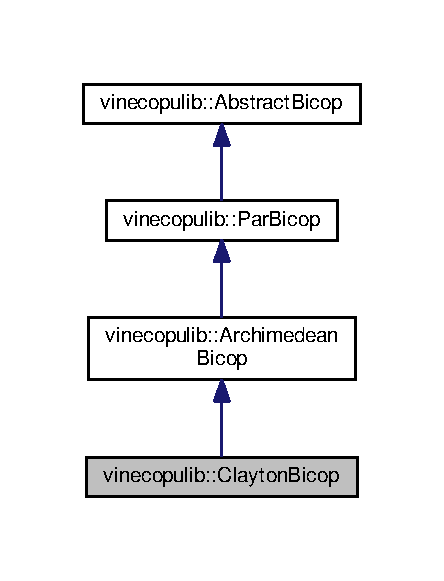
\includegraphics[width=210pt]{classvinecopulib_1_1_clayton_bicop__inherit__graph}
\end{center}
\end{figure}


Collaboration diagram for vinecopulib\+:\+:Clayton\+Bicop\+:\nopagebreak
\begin{figure}[H]
\begin{center}
\leavevmode
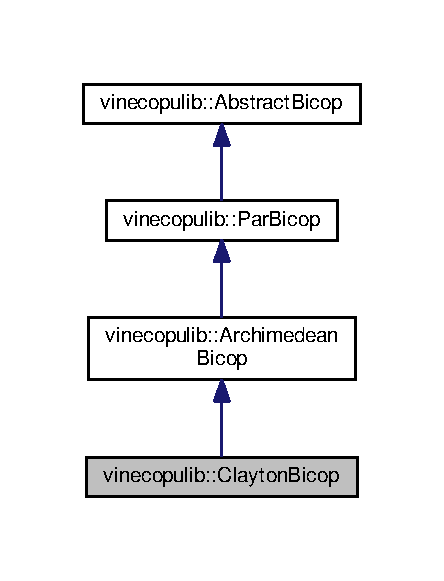
\includegraphics[width=210pt]{classvinecopulib_1_1_clayton_bicop__coll__graph}
\end{center}
\end{figure}
\subsection*{Additional Inherited Members}


The documentation for this class was generated from the following files\+:\begin{DoxyCompactItemize}
\item 
/home/n5/dev/cpp/vinecopulib/include/bicop\+\_\+clayton.\+hpp\item 
/home/n5/dev/cpp/vinecopulib/src/bicop\+\_\+clayton.\+cpp\end{DoxyCompactItemize}

\hypertarget{classvinecopulib_1_1_elliptical_bicop}{}\section{vinecopulib\+:\+:Elliptical\+Bicop Class Reference}
\label{classvinecopulib_1_1_elliptical_bicop}\index{vinecopulib\+::\+Elliptical\+Bicop@{vinecopulib\+::\+Elliptical\+Bicop}}


An abstract class for elliptical copula families.  




{\ttfamily \#include $<$elliptical.\+hpp$>$}



Inheritance diagram for vinecopulib\+:\+:Elliptical\+Bicop\+:\nopagebreak
\begin{figure}[H]
\begin{center}
\leavevmode
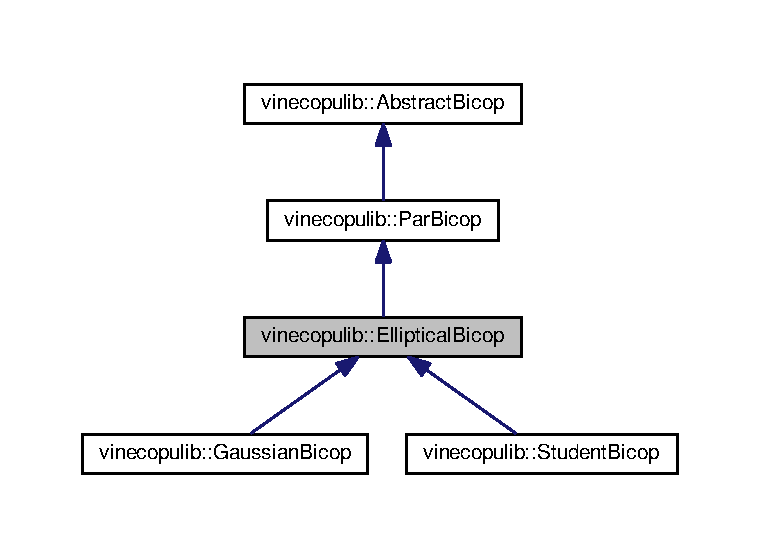
\includegraphics[width=350pt]{classvinecopulib_1_1_elliptical_bicop__inherit__graph}
\end{center}
\end{figure}


Collaboration diagram for vinecopulib\+:\+:Elliptical\+Bicop\+:\nopagebreak
\begin{figure}[H]
\begin{center}
\leavevmode
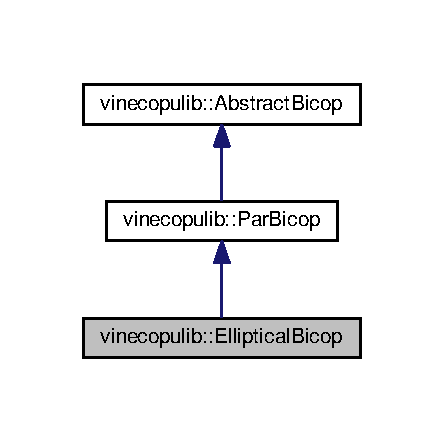
\includegraphics[width=213pt]{classvinecopulib_1_1_elliptical_bicop__coll__graph}
\end{center}
\end{figure}
\subsection*{Additional Inherited Members}


\subsection{Detailed Description}
An abstract class for elliptical copula families. 

This class is used in the implementation underlying the \hyperlink{classvinecopulib_1_1_bicop}{Bicop} class. Users should not use \hyperlink{classvinecopulib_1_1_abstract_bicop}{Abstract\+Bicop} or derived classes directly, but always work with the \hyperlink{classvinecopulib_1_1_bicop}{Bicop} interface.

Joe, Harry. Dependence modeling with copulas. C\+RC Press, 2014. 

The documentation for this class was generated from the following files\+:\begin{DoxyCompactItemize}
\item 
/home/n5/dev/cpp/vinecopulib/include/vinecopulib/bicop/elliptical.\+hpp\item 
/home/n5/dev/cpp/vinecopulib/src/bicop/elliptical.\+cpp\end{DoxyCompactItemize}

\hypertarget{classvinecopulib_1_1_fit_controls_bicop}{}\section{vinecopulib\+:\+:Fit\+Controls\+Bicop Class Reference}
\label{classvinecopulib_1_1_fit_controls_bicop}\index{vinecopulib\+::\+Fit\+Controls\+Bicop@{vinecopulib\+::\+Fit\+Controls\+Bicop}}


A class for controlling fit of bivariate copula models.  




{\ttfamily \#include $<$fit\+\_\+controls.\+hpp$>$}



Inheritance diagram for vinecopulib\+:\+:Fit\+Controls\+Bicop\+:\nopagebreak
\begin{figure}[H]
\begin{center}
\leavevmode
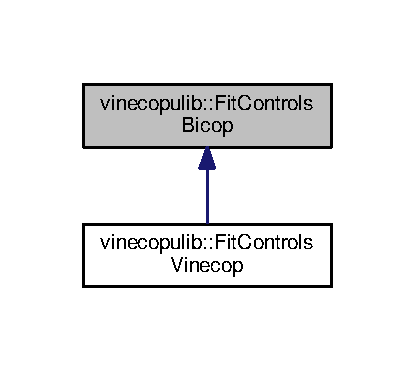
\includegraphics[width=199pt]{classvinecopulib_1_1_fit_controls_bicop__inherit__graph}
\end{center}
\end{figure}
\subsection*{Public Member Functions}
\begin{DoxyCompactItemize}
\item 
\hyperlink{classvinecopulib_1_1_fit_controls_bicop_a544d095b0ef0a99e08b8ca60a5753fbe}{Fit\+Controls\+Bicop} (std\+::vector$<$ \hyperlink{namespacevinecopulib_a42e95cc06d33896199caab0c11ad44f3}{Bicop\+Family} $>$ family\+\_\+set=\hyperlink{namespacevinecopulib_1_1bicop__families_a5214a513f41ec23b74782aab96ea6774}{bicop\+\_\+families\+::all}, std\+::string parametric\+\_\+method=\char`\"{}mle\char`\"{}, double nonparametric\+\_\+mult=1.\+0, std\+::string selection\+\_\+criterion=\char`\"{}bic\char`\"{}, bool preselect\+\_\+families=true)
\end{DoxyCompactItemize}
{\bf }\par
\begin{DoxyCompactItemize}
\item 
std\+::vector$<$ \hyperlink{namespacevinecopulib_a42e95cc06d33896199caab0c11ad44f3}{Bicop\+Family} $>$ \hyperlink{classvinecopulib_1_1_fit_controls_bicop_a8ea096aec62cbca55641941c9b4cf8f8}{get\+\_\+family\+\_\+set} () const 
\item 
std\+::string {\bfseries get\+\_\+parametric\+\_\+method} () const \hypertarget{classvinecopulib_1_1_fit_controls_bicop_a7399d0e67b734aeca98e47a8527ffea2}{}\label{classvinecopulib_1_1_fit_controls_bicop_a7399d0e67b734aeca98e47a8527ffea2}

\item 
double {\bfseries get\+\_\+nonparametric\+\_\+mult} () const \hypertarget{classvinecopulib_1_1_fit_controls_bicop_a8358f3bf302abf5dcbc646b8ea6493bd}{}\label{classvinecopulib_1_1_fit_controls_bicop_a8358f3bf302abf5dcbc646b8ea6493bd}

\item 
std\+::string {\bfseries get\+\_\+selection\+\_\+criterion} () const \hypertarget{classvinecopulib_1_1_fit_controls_bicop_ae05604585084979bc8637aa7af881eab}{}\label{classvinecopulib_1_1_fit_controls_bicop_ae05604585084979bc8637aa7af881eab}

\item 
bool {\bfseries get\+\_\+preselect\+\_\+families} () const \hypertarget{classvinecopulib_1_1_fit_controls_bicop_a9f5a3c90dc779f4f0f694869e62e6240}{}\label{classvinecopulib_1_1_fit_controls_bicop_a9f5a3c90dc779f4f0f694869e62e6240}

\item 
void {\bfseries set\+\_\+family\+\_\+set} (std\+::vector$<$ \hyperlink{namespacevinecopulib_a42e95cc06d33896199caab0c11ad44f3}{Bicop\+Family} $>$ family\+\_\+set)\hypertarget{classvinecopulib_1_1_fit_controls_bicop_a39d4e24261da184abf3fa3dd11d1f23b}{}\label{classvinecopulib_1_1_fit_controls_bicop_a39d4e24261da184abf3fa3dd11d1f23b}

\item 
void {\bfseries set\+\_\+parametric\+\_\+method} (std\+::string parametric\+\_\+method)\hypertarget{classvinecopulib_1_1_fit_controls_bicop_a722bef09427577ba2f04c91d7e4dba90}{}\label{classvinecopulib_1_1_fit_controls_bicop_a722bef09427577ba2f04c91d7e4dba90}

\item 
void {\bfseries set\+\_\+nonparametric\+\_\+mult} (double nonparametric\+\_\+mult)\hypertarget{classvinecopulib_1_1_fit_controls_bicop_a69fa1ff241282cc5a968ff64f0029ae0}{}\label{classvinecopulib_1_1_fit_controls_bicop_a69fa1ff241282cc5a968ff64f0029ae0}

\item 
void {\bfseries set\+\_\+selection\+\_\+criterion} (std\+::string selection\+\_\+criterion)\hypertarget{classvinecopulib_1_1_fit_controls_bicop_a52c187e5fcf047825ced777d73483df1}{}\label{classvinecopulib_1_1_fit_controls_bicop_a52c187e5fcf047825ced777d73483df1}

\item 
void {\bfseries set\+\_\+preselect\+\_\+families} (bool preselect\+\_\+families)\hypertarget{classvinecopulib_1_1_fit_controls_bicop_a7850b5ba8acaf78109d00789d93cc876}{}\label{classvinecopulib_1_1_fit_controls_bicop_a7850b5ba8acaf78109d00789d93cc876}

\end{DoxyCompactItemize}



\subsection{Detailed Description}
A class for controlling fit of bivariate copula models. 

\subsection{Constructor \& Destructor Documentation}
\index{vinecopulib\+::\+Fit\+Controls\+Bicop@{vinecopulib\+::\+Fit\+Controls\+Bicop}!Fit\+Controls\+Bicop@{Fit\+Controls\+Bicop}}
\index{Fit\+Controls\+Bicop@{Fit\+Controls\+Bicop}!vinecopulib\+::\+Fit\+Controls\+Bicop@{vinecopulib\+::\+Fit\+Controls\+Bicop}}
\subsubsection[{\texorpdfstring{Fit\+Controls\+Bicop(std\+::vector$<$ Bicop\+Family $>$ family\+\_\+set=bicop\+\_\+families\+::all, std\+::string parametric\+\_\+method=""mle"", double nonparametric\+\_\+mult=1.\+0, std\+::string selection\+\_\+criterion=""bic"", bool preselect\+\_\+families=true)}{FitControlsBicop(std::vector< BicopFamily > family_set=bicop_families::all, std::string parametric_method="mle", double nonparametric_mult=1.0, std::string selection_criterion="bic", bool preselect_families=true)}}]{\setlength{\rightskip}{0pt plus 5cm}vinecopulib\+::\+Fit\+Controls\+Bicop\+::\+Fit\+Controls\+Bicop (
\begin{DoxyParamCaption}
\item[{std\+::vector$<$ {\bf Bicop\+Family} $>$}]{family\+\_\+set = {\ttfamily {\bf bicop\+\_\+families\+::all}}, }
\item[{std\+::string}]{parametric\+\_\+method = {\ttfamily \char`\"{}mle\char`\"{}}, }
\item[{double}]{nonparametric\+\_\+mult = {\ttfamily 1.0}, }
\item[{std\+::string}]{selection\+\_\+criterion = {\ttfamily \char`\"{}bic\char`\"{}}, }
\item[{bool}]{preselect\+\_\+families = {\ttfamily true}}
\end{DoxyParamCaption}
)}\hypertarget{classvinecopulib_1_1_fit_controls_bicop_a544d095b0ef0a99e08b8ca60a5753fbe}{}\label{classvinecopulib_1_1_fit_controls_bicop_a544d095b0ef0a99e08b8ca60a5753fbe}
creates the controls for fitting bivariate copula models. 
\begin{DoxyParams}{Parameters}
{\em family\+\_\+set} & the set of copula families to consider (if empty, then all families are included). \\
\hline
{\em parametric\+\_\+method} & the fit method for parametric families; possible choices\+: {\ttfamily \char`\"{}mle\char`\"{}}, {\ttfamily \char`\"{}itau\char`\"{}}. \\
\hline
{\em nonparametric\+\_\+mult} & a factor with which the smoothing parameters are multiplied. \\
\hline
{\em selection\+\_\+criterion} & the selection criterion ({\ttfamily \char`\"{}aic\char`\"{}} or {\ttfamily \char`\"{}bic\char`\"{}}). \\
\hline
{\em preselect\+\_\+families} & whether to exclude families before fitting based on symmetry properties of the data. \\
\hline
\end{DoxyParams}


\subsection{Member Function Documentation}
\index{vinecopulib\+::\+Fit\+Controls\+Bicop@{vinecopulib\+::\+Fit\+Controls\+Bicop}!get\+\_\+family\+\_\+set@{get\+\_\+family\+\_\+set}}
\index{get\+\_\+family\+\_\+set@{get\+\_\+family\+\_\+set}!vinecopulib\+::\+Fit\+Controls\+Bicop@{vinecopulib\+::\+Fit\+Controls\+Bicop}}
\subsubsection[{\texorpdfstring{get\+\_\+family\+\_\+set() const }{get_family_set() const }}]{\setlength{\rightskip}{0pt plus 5cm}std\+::vector$<$ {\bf Bicop\+Family} $>$ vinecopulib\+::\+Fit\+Controls\+Bicop\+::get\+\_\+family\+\_\+set (
\begin{DoxyParamCaption}
{}
\end{DoxyParamCaption}
) const}\hypertarget{classvinecopulib_1_1_fit_controls_bicop_a8ea096aec62cbca55641941c9b4cf8f8}{}\label{classvinecopulib_1_1_fit_controls_bicop_a8ea096aec62cbca55641941c9b4cf8f8}
Getters and setters. 

The documentation for this class was generated from the following files\+:\begin{DoxyCompactItemize}
\item 
/home/n5/dev/cpp/vinecopulib/include/bicop/fit\+\_\+controls.\+hpp\item 
/home/n5/dev/cpp/vinecopulib/src/bicop/fit\+\_\+controls.\+cpp\end{DoxyCompactItemize}

\hypertarget{classvinecopulib_1_1_fit_controls_vinecop}{}\section{vinecopulib\+:\+:Fit\+Controls\+Vinecop Class Reference}
\label{classvinecopulib_1_1_fit_controls_vinecop}\index{vinecopulib\+::\+Fit\+Controls\+Vinecop@{vinecopulib\+::\+Fit\+Controls\+Vinecop}}


A class for controlling fit of bivariate copula models.  




{\ttfamily \#include $<$fit\+\_\+controls.\+hpp$>$}



Inheritance diagram for vinecopulib\+:\+:Fit\+Controls\+Vinecop\+:\nopagebreak
\begin{figure}[H]
\begin{center}
\leavevmode
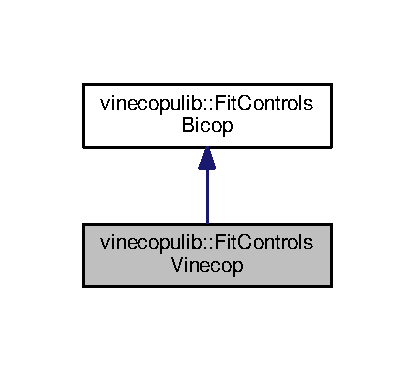
\includegraphics[width=199pt]{classvinecopulib_1_1_fit_controls_vinecop__inherit__graph}
\end{center}
\end{figure}


Collaboration diagram for vinecopulib\+:\+:Fit\+Controls\+Vinecop\+:\nopagebreak
\begin{figure}[H]
\begin{center}
\leavevmode
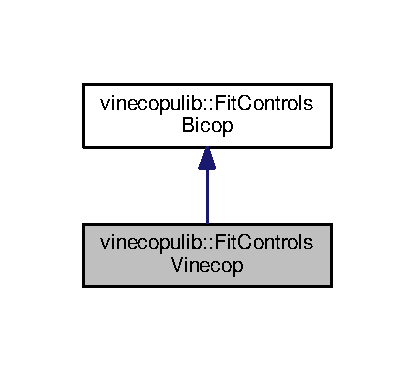
\includegraphics[width=199pt]{classvinecopulib_1_1_fit_controls_vinecop__coll__graph}
\end{center}
\end{figure}
\subsection*{Public Member Functions}
\begin{DoxyCompactItemize}
\item 
\hyperlink{classvinecopulib_1_1_fit_controls_vinecop_ad101d135c8d8fe66046d931947f45bef}{Fit\+Controls\+Vinecop} ()\hypertarget{classvinecopulib_1_1_fit_controls_vinecop_ad101d135c8d8fe66046d931947f45bef}{}\label{classvinecopulib_1_1_fit_controls_vinecop_ad101d135c8d8fe66046d931947f45bef}

\begin{DoxyCompactList}\small\item\em creates default controls for fitting vine copula models. \end{DoxyCompactList}\item 
\hyperlink{classvinecopulib_1_1_fit_controls_vinecop_af0550d369be595665d0d9e8f6709a74c}{Fit\+Controls\+Vinecop} (std\+::vector$<$ \hyperlink{namespacevinecopulib_a42e95cc06d33896199caab0c11ad44f3}{Bicop\+Family} $>$ family\+\_\+set, std\+::string parametric\+\_\+method=\char`\"{}mle\char`\"{}, std\+::string nonparametric\+\_\+method=\char`\"{}quadratic\char`\"{}, double nonparametric\+\_\+mult=1.\+0, size\+\_\+t truncation\+\_\+level=std\+::numeric\+\_\+limits$<$ size\+\_\+t $>$\+::max(), std\+::string tree\+\_\+criterion=\char`\"{}tau\char`\"{}, double threshold=0.\+0, std\+::string selection\+\_\+criterion=\char`\"{}bic\char`\"{}, bool preselect\+\_\+families=true, bool select\+\_\+truncation\+\_\+level=false, bool select\+\_\+threshold=false, bool show\+\_\+trace=false)
\item 
\hyperlink{classvinecopulib_1_1_fit_controls_vinecop_a21e1351edcb735b959342384f3dae212}{Fit\+Controls\+Vinecop} (const \hyperlink{classvinecopulib_1_1_fit_controls_bicop}{Fit\+Controls\+Bicop} controls, size\+\_\+t truncation\+\_\+level=std\+::numeric\+\_\+limits$<$ size\+\_\+t $>$\+::max(), std\+::string tree\+\_\+criterion=\char`\"{}tau\char`\"{}, double threshold=0.\+0, bool select\+\_\+truncation\+\_\+level=false, bool select\+\_\+threshold=false, bool show\+\_\+trace=false)
\end{DoxyCompactItemize}
{\bf }\par
\begin{DoxyCompactItemize}
\item 
size\+\_\+t \hyperlink{classvinecopulib_1_1_fit_controls_vinecop_afa52dd1f64f6a89ba59ad80374c268a0}{get\+\_\+truncation\+\_\+level} ()
\end{DoxyCompactItemize}



\subsection{Detailed Description}
A class for controlling fit of bivariate copula models. 

\subsection{Constructor \& Destructor Documentation}
\index{vinecopulib\+::\+Fit\+Controls\+Vinecop@{vinecopulib\+::\+Fit\+Controls\+Vinecop}!Fit\+Controls\+Vinecop@{Fit\+Controls\+Vinecop}}
\index{Fit\+Controls\+Vinecop@{Fit\+Controls\+Vinecop}!vinecopulib\+::\+Fit\+Controls\+Vinecop@{vinecopulib\+::\+Fit\+Controls\+Vinecop}}
\subsubsection[{\texorpdfstring{Fit\+Controls\+Vinecop(std\+::vector$<$ Bicop\+Family $>$ family\+\_\+set, std\+::string parametric\+\_\+method=""mle"", std\+::string nonparametric\+\_\+method=""quadratic"", double nonparametric\+\_\+mult=1.\+0, size\+\_\+t truncation\+\_\+level=std\+::numeric\+\_\+limits$<$ size\+\_\+t $>$\+::max(), std\+::string tree\+\_\+criterion=""tau"", double threshold=0.\+0, std\+::string selection\+\_\+criterion=""bic"", bool preselect\+\_\+families=true, bool select\+\_\+truncation\+\_\+level=false, bool select\+\_\+threshold=false, bool show\+\_\+trace=false)}{FitControlsVinecop(std::vector< BicopFamily > family_set, std::string parametric_method="mle", std::string nonparametric_method="quadratic", double nonparametric_mult=1.0, size_t truncation_level=std::numeric_limits< size_t >::max(), std::string tree_criterion="tau", double threshold=0.0, std::string selection_criterion="bic", bool preselect_families=true, bool select_truncation_level=false, bool select_threshold=false, bool show_trace=false)}}]{\setlength{\rightskip}{0pt plus 5cm}vinecopulib\+::\+Fit\+Controls\+Vinecop\+::\+Fit\+Controls\+Vinecop (
\begin{DoxyParamCaption}
\item[{std\+::vector$<$ {\bf Bicop\+Family} $>$}]{family\+\_\+set, }
\item[{std\+::string}]{parametric\+\_\+method = {\ttfamily \char`\"{}mle\char`\"{}}, }
\item[{std\+::string}]{nonparametric\+\_\+method = {\ttfamily \char`\"{}quadratic\char`\"{}}, }
\item[{double}]{nonparametric\+\_\+mult = {\ttfamily 1.0}, }
\item[{size\+\_\+t}]{truncation\+\_\+level = {\ttfamily std\+:\+:numeric\+\_\+limits$<$size\+\_\+t$>$\+:\+:max()}, }
\item[{std\+::string}]{tree\+\_\+criterion = {\ttfamily \char`\"{}tau\char`\"{}}, }
\item[{double}]{threshold = {\ttfamily 0.0}, }
\item[{std\+::string}]{selection\+\_\+criterion = {\ttfamily \char`\"{}bic\char`\"{}}, }
\item[{bool}]{preselect\+\_\+families = {\ttfamily true}, }
\item[{bool}]{select\+\_\+truncation\+\_\+level = {\ttfamily false}, }
\item[{bool}]{select\+\_\+threshold = {\ttfamily false}, }
\item[{bool}]{show\+\_\+trace = {\ttfamily false}}
\end{DoxyParamCaption}
)}\hypertarget{classvinecopulib_1_1_fit_controls_vinecop_af0550d369be595665d0d9e8f6709a74c}{}\label{classvinecopulib_1_1_fit_controls_vinecop_af0550d369be595665d0d9e8f6709a74c}
creates custom controls for fitting vine copula models. 
\begin{DoxyParams}{Parameters}
{\em family\+\_\+set} & see \hyperlink{classvinecopulib_1_1_fit_controls_bicop}{Fit\+Controls\+Bicop}. \\
\hline
{\em parametric\+\_\+method} & see \hyperlink{classvinecopulib_1_1_fit_controls_bicop}{Fit\+Controls\+Bicop}. \\
\hline
{\em nonparametric\+\_\+method} & see \hyperlink{classvinecopulib_1_1_fit_controls_bicop}{Fit\+Controls\+Bicop}. \\
\hline
{\em nonparametric\+\_\+mult} & see \hyperlink{classvinecopulib_1_1_fit_controls_bicop}{Fit\+Controls\+Bicop}. \\
\hline
{\em truncation\+\_\+level} & for truncated vines. \\
\hline
{\em tree\+\_\+criterion} & the criterion for selecting the maximum spanning tree (\char`\"{}tau\char`\"{}, \char`\"{}hoeffd\char`\"{} and \char`\"{}rho\char`\"{} implemented so far). \\
\hline
{\em threshold} & for thresholded vines (0 = no threshold). \\
\hline
{\em selection\+\_\+criterion} & see \hyperlink{classvinecopulib_1_1_fit_controls_bicop}{Fit\+Controls\+Bicop}. \\
\hline
{\em preselect\+\_\+families} & see \hyperlink{classvinecopulib_1_1_fit_controls_bicop}{Fit\+Controls\+Bicop}. \\
\hline
{\em select\+\_\+truncation\+\_\+level} & whether the truncation shall be selected automatically. \\
\hline
{\em select\+\_\+threshold} & whether the threshold parameter shall be selected automatically. \\
\hline
{\em show\+\_\+trace} & whether to show a trace of the building progress. \\
\hline
\end{DoxyParams}
\index{vinecopulib\+::\+Fit\+Controls\+Vinecop@{vinecopulib\+::\+Fit\+Controls\+Vinecop}!Fit\+Controls\+Vinecop@{Fit\+Controls\+Vinecop}}
\index{Fit\+Controls\+Vinecop@{Fit\+Controls\+Vinecop}!vinecopulib\+::\+Fit\+Controls\+Vinecop@{vinecopulib\+::\+Fit\+Controls\+Vinecop}}
\subsubsection[{\texorpdfstring{Fit\+Controls\+Vinecop(const Fit\+Controls\+Bicop controls, size\+\_\+t truncation\+\_\+level=std\+::numeric\+\_\+limits$<$ size\+\_\+t $>$\+::max(), std\+::string tree\+\_\+criterion=""tau"", double threshold=0.\+0, bool select\+\_\+truncation\+\_\+level=false, bool select\+\_\+threshold=false, bool show\+\_\+trace=false)}{FitControlsVinecop(const FitControlsBicop controls, size_t truncation_level=std::numeric_limits< size_t >::max(), std::string tree_criterion="tau", double threshold=0.0, bool select_truncation_level=false, bool select_threshold=false, bool show_trace=false)}}]{\setlength{\rightskip}{0pt plus 5cm}vinecopulib\+::\+Fit\+Controls\+Vinecop\+::\+Fit\+Controls\+Vinecop (
\begin{DoxyParamCaption}
\item[{const {\bf Fit\+Controls\+Bicop}}]{controls, }
\item[{size\+\_\+t}]{truncation\+\_\+level = {\ttfamily std\+:\+:numeric\+\_\+limits$<$size\+\_\+t$>$\+:\+:max()}, }
\item[{std\+::string}]{tree\+\_\+criterion = {\ttfamily \char`\"{}tau\char`\"{}}, }
\item[{double}]{threshold = {\ttfamily 0.0}, }
\item[{bool}]{select\+\_\+truncation\+\_\+level = {\ttfamily false}, }
\item[{bool}]{select\+\_\+threshold = {\ttfamily false}, }
\item[{bool}]{show\+\_\+trace = {\ttfamily false}}
\end{DoxyParamCaption}
)}\hypertarget{classvinecopulib_1_1_fit_controls_vinecop_a21e1351edcb735b959342384f3dae212}{}\label{classvinecopulib_1_1_fit_controls_vinecop_a21e1351edcb735b959342384f3dae212}
creates custom controls for fitting vine copula models. 
\begin{DoxyParams}{Parameters}
{\em truncation\+\_\+level} & for truncated vines. \\
\hline
{\em tree\+\_\+criterion} & the criterion for selecting the maximum spanning tree (\char`\"{}tau\char`\"{}, \char`\"{}hoeffd\char`\"{} and \char`\"{}rho\char`\"{} implemented so far). \\
\hline
{\em threshold} & for thresholded vines (0 = no threshold). \\
\hline
{\em show\+\_\+trace} & whether to show a trace of the building progress. \\
\hline
{\em select\+\_\+truncation\+\_\+level} & whether the truncation shall be selected automatically. \\
\hline
{\em select\+\_\+threshold} & whether the threshold parameter shall be selected automatically. \\
\hline
{\em controls} & see \hyperlink{classvinecopulib_1_1_fit_controls_bicop}{Fit\+Controls\+Bicop}. \\
\hline
\end{DoxyParams}


\subsection{Member Function Documentation}
\index{vinecopulib\+::\+Fit\+Controls\+Vinecop@{vinecopulib\+::\+Fit\+Controls\+Vinecop}!get\+\_\+truncation\+\_\+level@{get\+\_\+truncation\+\_\+level}}
\index{get\+\_\+truncation\+\_\+level@{get\+\_\+truncation\+\_\+level}!vinecopulib\+::\+Fit\+Controls\+Vinecop@{vinecopulib\+::\+Fit\+Controls\+Vinecop}}
\subsubsection[{\texorpdfstring{get\+\_\+truncation\+\_\+level()}{get_truncation_level()}}]{\setlength{\rightskip}{0pt plus 5cm}size\+\_\+t vinecopulib\+::\+Fit\+Controls\+Vinecop\+::get\+\_\+truncation\+\_\+level (
\begin{DoxyParamCaption}
{}
\end{DoxyParamCaption}
)}\hypertarget{classvinecopulib_1_1_fit_controls_vinecop_afa52dd1f64f6a89ba59ad80374c268a0}{}\label{classvinecopulib_1_1_fit_controls_vinecop_afa52dd1f64f6a89ba59ad80374c268a0}
Getters and setters. 

The documentation for this class was generated from the following files\+:\begin{DoxyCompactItemize}
\item 
vinecopulib/include/vinecopulib/vinecop/fit\+\_\+controls.\+hpp\item 
vinecopulib/src/vinecop/fit\+\_\+controls.\+cpp\end{DoxyCompactItemize}

\hypertarget{classvinecopulib_1_1_frank_bicop}{}\section{vinecopulib\+:\+:Frank\+Bicop Class Reference}
\label{classvinecopulib_1_1_frank_bicop}\index{vinecopulib\+::\+Frank\+Bicop@{vinecopulib\+::\+Frank\+Bicop}}


The Frank copula.  




{\ttfamily \#include $<$frank.\+hpp$>$}



Inheritance diagram for vinecopulib\+:\+:Frank\+Bicop\+:
\nopagebreak
\begin{figure}[H]
\begin{center}
\leavevmode
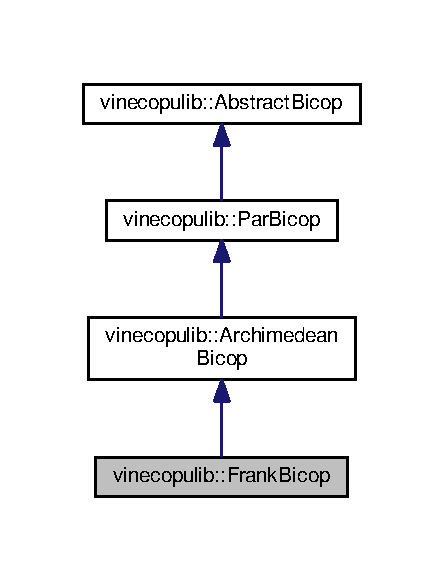
\includegraphics[width=213pt]{classvinecopulib_1_1_frank_bicop__inherit__graph}
\end{center}
\end{figure}


Collaboration diagram for vinecopulib\+:\+:Frank\+Bicop\+:
\nopagebreak
\begin{figure}[H]
\begin{center}
\leavevmode
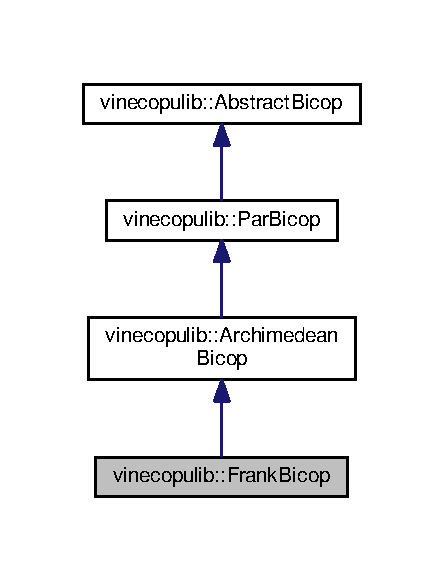
\includegraphics[width=213pt]{classvinecopulib_1_1_frank_bicop__coll__graph}
\end{center}
\end{figure}
\subsection*{Additional Inherited Members}


\subsection{Detailed Description}
The Frank copula. 

This class is used in the implementation underlying the \hyperlink{classvinecopulib_1_1_bicop}{Bicop} class. Users should not use \hyperlink{classvinecopulib_1_1_abstract_bicop}{Abstract\+Bicop} or derived classes directly, but always work with the \hyperlink{classvinecopulib_1_1_bicop}{Bicop} interface.

Joe, Harry. Dependence modeling with copulas. C\+RC Press, 2014. 

The documentation for this class was generated from the following files\+:\begin{DoxyCompactItemize}
\item 
/home/n5/dev/cpp/vinecopulib/include/bicop/frank.\+hpp\item 
/home/n5/dev/cpp/vinecopulib/src/bicop/frank.\+cpp\end{DoxyCompactItemize}

\hypertarget{classvinecopulib_1_1_gaussian_bicop}{}\section{vinecopulib\+:\+:Gaussian\+Bicop Class Reference}
\label{classvinecopulib_1_1_gaussian_bicop}\index{vinecopulib\+::\+Gaussian\+Bicop@{vinecopulib\+::\+Gaussian\+Bicop}}


The Gaussian copula.  




{\ttfamily \#include $<$gaussian.\+hpp$>$}



Inheritance diagram for vinecopulib\+:\+:Gaussian\+Bicop\+:\nopagebreak
\begin{figure}[H]
\begin{center}
\leavevmode
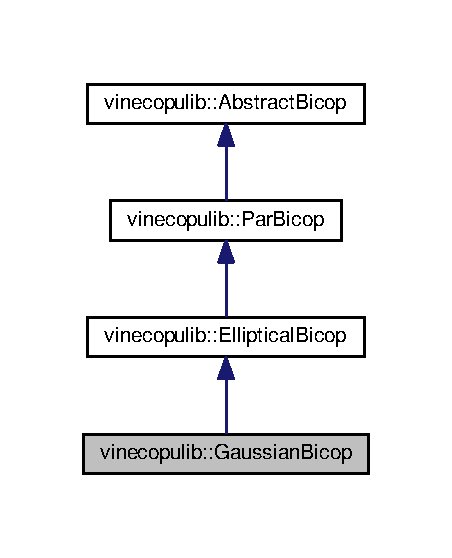
\includegraphics[width=217pt]{classvinecopulib_1_1_gaussian_bicop__inherit__graph}
\end{center}
\end{figure}


Collaboration diagram for vinecopulib\+:\+:Gaussian\+Bicop\+:\nopagebreak
\begin{figure}[H]
\begin{center}
\leavevmode
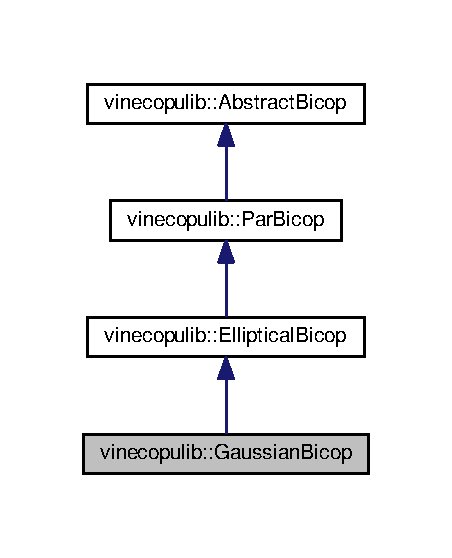
\includegraphics[width=217pt]{classvinecopulib_1_1_gaussian_bicop__coll__graph}
\end{center}
\end{figure}
\subsection*{Additional Inherited Members}


\subsection{Detailed Description}
The Gaussian copula. 

This class is used in the implementation underlying the \hyperlink{classvinecopulib_1_1_bicop}{Bicop} class. Users should not use \hyperlink{classvinecopulib_1_1_abstract_bicop}{Abstract\+Bicop} or derived classes directly, but always work with the \hyperlink{classvinecopulib_1_1_bicop}{Bicop} interface.

Joe, Harry. Dependence modeling with copulas. C\+RC Press, 2014. 

The documentation for this class was generated from the following files\+:\begin{DoxyCompactItemize}
\item 
/home/n5/dev/cpp/vinecopulib/include/vinecopulib/bicop/gaussian.\+hpp\item 
/home/n5/dev/cpp/vinecopulib/src/bicop/gaussian.\+cpp\end{DoxyCompactItemize}

\hypertarget{classvinecopulib_1_1_gumbel_bicop}{\section{vinecopulib\+:\+:Gumbel\+Bicop Class Reference}
\label{classvinecopulib_1_1_gumbel_bicop}\index{vinecopulib\+::\+Gumbel\+Bicop@{vinecopulib\+::\+Gumbel\+Bicop}}
}


The Gumbel copula.  




{\ttfamily \#include $<$gumbel.\+hpp$>$}



Inheritance diagram for vinecopulib\+:\+:Gumbel\+Bicop\+:\nopagebreak
\begin{figure}[H]
\begin{center}
\leavevmode
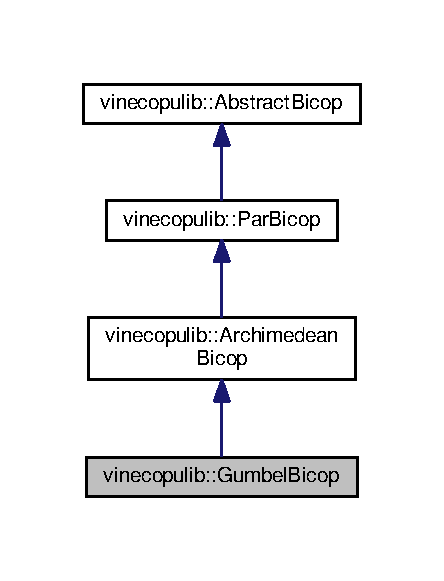
\includegraphics[width=212pt]{classvinecopulib_1_1_gumbel_bicop__inherit__graph}
\end{center}
\end{figure}


Collaboration diagram for vinecopulib\+:\+:Gumbel\+Bicop\+:\nopagebreak
\begin{figure}[H]
\begin{center}
\leavevmode
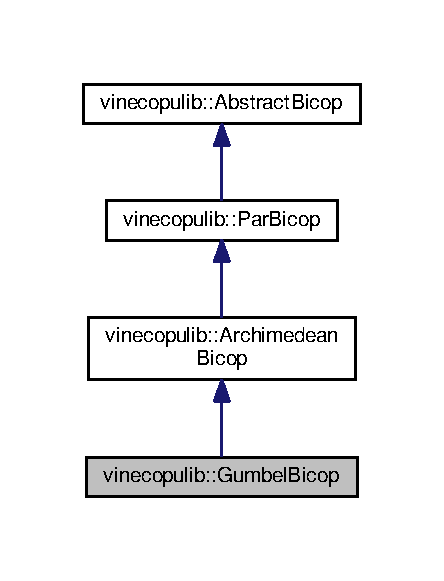
\includegraphics[width=212pt]{classvinecopulib_1_1_gumbel_bicop__coll__graph}
\end{center}
\end{figure}
\subsection*{Additional Inherited Members}


\subsection{Detailed Description}
The Gumbel copula. 

This class is used in the implementation underlying the \hyperlink{classvinecopulib_1_1_bicop}{Bicop} class. Users should not use \hyperlink{classvinecopulib_1_1_abstract_bicop}{Abstract\+Bicop} or derived classes directly, but always work with the \hyperlink{classvinecopulib_1_1_bicop}{Bicop} interface.

Joe, Harry. Dependence modeling with copulas. C\+R\+C Press, 2014. 

The documentation for this class was generated from the following files\+:\begin{DoxyCompactItemize}
\item 
vinecopulib/include/vinecopulib/bicop/gumbel.\+hpp\item 
vinecopulib/src/bicop/gumbel.\+cpp\end{DoxyCompactItemize}

\hypertarget{classvinecopulib_1_1_indep_bicop}{}\section{vinecopulib\+:\+:Indep\+Bicop Class Reference}
\label{classvinecopulib_1_1_indep_bicop}\index{vinecopulib\+::\+Indep\+Bicop@{vinecopulib\+::\+Indep\+Bicop}}


The independence copula.  




{\ttfamily \#include $<$indep.\+hpp$>$}



Inheritance diagram for vinecopulib\+:\+:Indep\+Bicop\+:\nopagebreak
\begin{figure}[H]
\begin{center}
\leavevmode
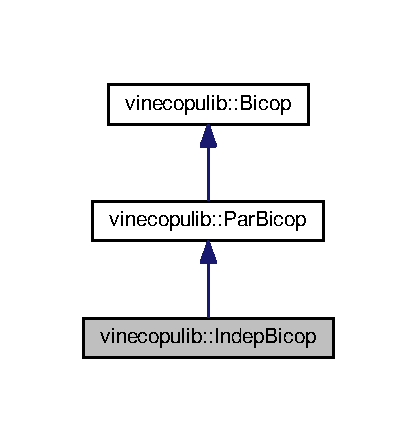
\includegraphics[width=213pt]{classvinecopulib_1_1_indep_bicop__inherit__graph}
\end{center}
\end{figure}


Collaboration diagram for vinecopulib\+:\+:Indep\+Bicop\+:\nopagebreak
\begin{figure}[H]
\begin{center}
\leavevmode
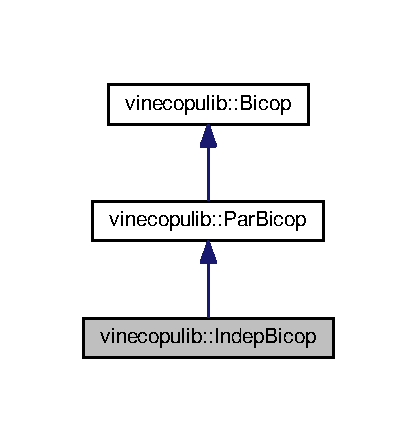
\includegraphics[width=213pt]{classvinecopulib_1_1_indep_bicop__coll__graph}
\end{center}
\end{figure}
\subsection*{Additional Inherited Members}


\subsection{Detailed Description}
The independence copula. 

This class is used in the implementation underlying the \hyperlink{classvinecopulib_1_1_bicop}{Bicop} class. Users should not use \hyperlink{classvinecopulib_1_1_abstract_bicop}{Abstract\+Bicop} or derived classes directly, but always work with the \hyperlink{classvinecopulib_1_1_bicop}{Bicop} interface.

Joe, Harry. Dependence modeling with copulas. C\+RC Press, 2014. 

The documentation for this class was generated from the following files\+:\begin{DoxyCompactItemize}
\item 
/home/n5/dev/cpp/vinecopulib/include/vinecopulib/bicop/indep.\+hpp\item 
/home/n5/dev/cpp/vinecopulib/src/bicop/indep.\+cpp\end{DoxyCompactItemize}

\hypertarget{classvinecopulib_1_1tools__interpolation_1_1_interpolation_grid}{}\section{vinecopulib\+:\+:tools\+\_\+interpolation\+:\+:Interpolation\+Grid Class Reference}
\label{classvinecopulib_1_1tools__interpolation_1_1_interpolation_grid}\index{vinecopulib\+::tools\+\_\+interpolation\+::\+Interpolation\+Grid@{vinecopulib\+::tools\+\_\+interpolation\+::\+Interpolation\+Grid}}


{\ttfamily \#include $<$tools\+\_\+interpolation.\+hpp$>$}

\subsection*{Public Member Functions}
\begin{DoxyCompactItemize}
\item 
\hyperlink{classvinecopulib_1_1tools__interpolation_1_1_interpolation_grid_a2cc351aee4b943dba785881b893b35b2}{Interpolation\+Grid} (const Eigen\+::\+Vector\+Xd \&grid\+\_\+points, const Eigen\+::\+Matrix\+Xd \&values)
\item 
void {\bfseries flip} ()\hypertarget{classvinecopulib_1_1tools__interpolation_1_1_interpolation_grid_a9eec97102cfbb146cda8f6f4d4fc0794}{}\label{classvinecopulib_1_1tools__interpolation_1_1_interpolation_grid_a9eec97102cfbb146cda8f6f4d4fc0794}

\item 
Eigen\+::\+Vector\+Xd \hyperlink{classvinecopulib_1_1tools__interpolation_1_1_interpolation_grid_adee449dd69cee82748f02f9133069fc1}{interpolate} (const Eigen\+::\+Matrix\+Xd \&x)
\item 
Eigen\+::\+Vector\+Xd \hyperlink{classvinecopulib_1_1tools__interpolation_1_1_interpolation_grid_abe7711ab9183964ce99f43dccb097299}{intergrate\+\_\+1d} (const Eigen\+::\+Matrix\+Xd \&u, size\+\_\+t cond\+\_\+var)
\end{DoxyCompactItemize}


\subsection{Detailed Description}
A class for cubic spline interpolation of bivariate copulas

The class is used for implementing kernel estimators. It makes storing the observations obsolete and allows for fast numerical integration. 

\subsection{Constructor \& Destructor Documentation}
\index{vinecopulib\+::tools\+\_\+interpolation\+::\+Interpolation\+Grid@{vinecopulib\+::tools\+\_\+interpolation\+::\+Interpolation\+Grid}!Interpolation\+Grid@{Interpolation\+Grid}}
\index{Interpolation\+Grid@{Interpolation\+Grid}!vinecopulib\+::tools\+\_\+interpolation\+::\+Interpolation\+Grid@{vinecopulib\+::tools\+\_\+interpolation\+::\+Interpolation\+Grid}}
\subsubsection[{\texorpdfstring{Interpolation\+Grid(const Eigen\+::\+Vector\+Xd \&grid\+\_\+points, const Eigen\+::\+Matrix\+Xd \&values)}{InterpolationGrid(const Eigen::VectorXd &grid_points, const Eigen::MatrixXd &values)}}]{\setlength{\rightskip}{0pt plus 5cm}vinecopulib\+::tools\+\_\+interpolation\+::\+Interpolation\+Grid\+::\+Interpolation\+Grid (
\begin{DoxyParamCaption}
\item[{const Eigen\+::\+Vector\+Xd \&}]{grid\+\_\+points, }
\item[{const Eigen\+::\+Matrix\+Xd \&}]{values}
\end{DoxyParamCaption}
)}\hypertarget{classvinecopulib_1_1tools__interpolation_1_1_interpolation_grid_a2cc351aee4b943dba785881b893b35b2}{}\label{classvinecopulib_1_1tools__interpolation_1_1_interpolation_grid_a2cc351aee4b943dba785881b893b35b2}
Constructor


\begin{DoxyParams}{Parameters}
{\em grid\+\_\+points} & an ascending sequence of grid\+\_\+points; used in both dimensions. \\
\hline
{\em values} & a dxd matrix of copula density values evaluated at (grid\+\_\+points\+\_\+i, grid\+\_\+points\+\_\+j). \\
\hline
\end{DoxyParams}


\subsection{Member Function Documentation}
\index{vinecopulib\+::tools\+\_\+interpolation\+::\+Interpolation\+Grid@{vinecopulib\+::tools\+\_\+interpolation\+::\+Interpolation\+Grid}!intergrate\+\_\+1d@{intergrate\+\_\+1d}}
\index{intergrate\+\_\+1d@{intergrate\+\_\+1d}!vinecopulib\+::tools\+\_\+interpolation\+::\+Interpolation\+Grid@{vinecopulib\+::tools\+\_\+interpolation\+::\+Interpolation\+Grid}}
\subsubsection[{\texorpdfstring{intergrate\+\_\+1d(const Eigen\+::\+Matrix\+Xd \&u, size\+\_\+t cond\+\_\+var)}{intergrate_1d(const Eigen::MatrixXd &u, size_t cond_var)}}]{\setlength{\rightskip}{0pt plus 5cm}Eigen\+::\+Vector\+Xd vinecopulib\+::tools\+\_\+interpolation\+::\+Interpolation\+Grid\+::intergrate\+\_\+1d (
\begin{DoxyParamCaption}
\item[{const Eigen\+::\+Matrix\+Xd \&}]{u, }
\item[{size\+\_\+t}]{cond\+\_\+var}
\end{DoxyParamCaption}
)}\hypertarget{classvinecopulib_1_1tools__interpolation_1_1_interpolation_grid_abe7711ab9183964ce99f43dccb097299}{}\label{classvinecopulib_1_1tools__interpolation_1_1_interpolation_grid_abe7711ab9183964ce99f43dccb097299}
Integrate the grid along one axis


\begin{DoxyParams}{Parameters}
{\em u} & mx2 matrix of evaluation points \\
\hline
{\em cond\+\_\+var} & either 1 or 2; the axis considered fixed. \\
\hline
\end{DoxyParams}
\index{vinecopulib\+::tools\+\_\+interpolation\+::\+Interpolation\+Grid@{vinecopulib\+::tools\+\_\+interpolation\+::\+Interpolation\+Grid}!interpolate@{interpolate}}
\index{interpolate@{interpolate}!vinecopulib\+::tools\+\_\+interpolation\+::\+Interpolation\+Grid@{vinecopulib\+::tools\+\_\+interpolation\+::\+Interpolation\+Grid}}
\subsubsection[{\texorpdfstring{interpolate(const Eigen\+::\+Matrix\+Xd \&x)}{interpolate(const Eigen::MatrixXd &x)}}]{\setlength{\rightskip}{0pt plus 5cm}Eigen\+::\+Vector\+Xd vinecopulib\+::tools\+\_\+interpolation\+::\+Interpolation\+Grid\+::interpolate (
\begin{DoxyParamCaption}
\item[{const Eigen\+::\+Matrix\+Xd \&}]{x}
\end{DoxyParamCaption}
)}\hypertarget{classvinecopulib_1_1tools__interpolation_1_1_interpolation_grid_adee449dd69cee82748f02f9133069fc1}{}\label{classvinecopulib_1_1tools__interpolation_1_1_interpolation_grid_adee449dd69cee82748f02f9133069fc1}
Interpolation in two dimensions


\begin{DoxyParams}{Parameters}
{\em x} & mx2 matrix of evaluation points. \\
\hline
\end{DoxyParams}


The documentation for this class was generated from the following files\+:\begin{DoxyCompactItemize}
\item 
/home/n5/dev/cpp/vinecopulib/include/vinecopulib/misc/tools\+\_\+interpolation.\+hpp\item 
/home/n5/dev/cpp/vinecopulib/src/misc/tools\+\_\+interpolation.\+cpp\end{DoxyCompactItemize}

\hypertarget{classvinecopulib_1_1_joe_bicop}{}\section{vinecopulib\+:\+:Joe\+Bicop Class Reference}
\label{classvinecopulib_1_1_joe_bicop}\index{vinecopulib\+::\+Joe\+Bicop@{vinecopulib\+::\+Joe\+Bicop}}


The Joe copula.  




{\ttfamily \#include $<$joe.\+hpp$>$}



Inheritance diagram for vinecopulib\+:\+:Joe\+Bicop\+:\nopagebreak
\begin{figure}[H]
\begin{center}
\leavevmode
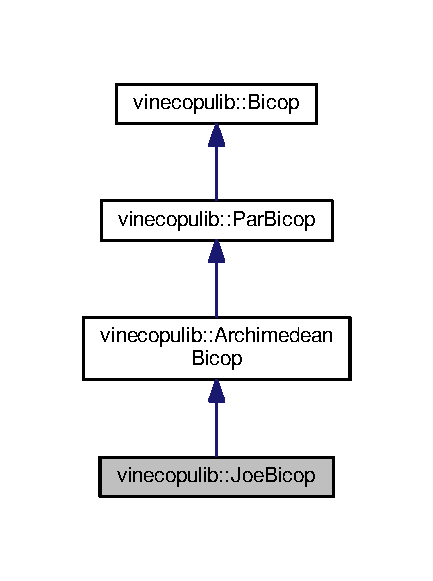
\includegraphics[width=213pt]{classvinecopulib_1_1_joe_bicop__inherit__graph}
\end{center}
\end{figure}


Collaboration diagram for vinecopulib\+:\+:Joe\+Bicop\+:\nopagebreak
\begin{figure}[H]
\begin{center}
\leavevmode
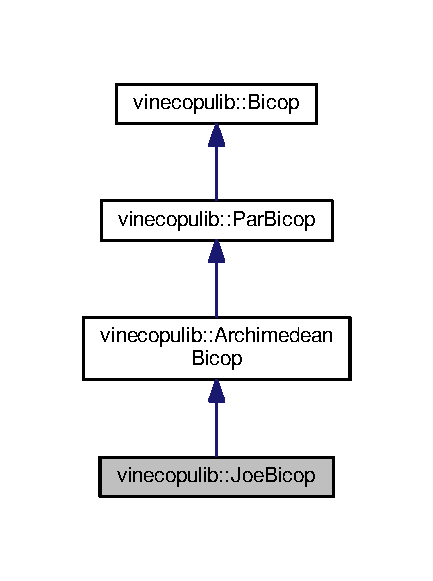
\includegraphics[width=213pt]{classvinecopulib_1_1_joe_bicop__coll__graph}
\end{center}
\end{figure}
\subsection*{Additional Inherited Members}


\subsection{Detailed Description}
The Joe copula. 

This class is used in the implementation underlying the \hyperlink{classvinecopulib_1_1_bicop}{Bicop} class. Users should not use \hyperlink{classvinecopulib_1_1_abstract_bicop}{Abstract\+Bicop} or derived classes directly, but always work with the \hyperlink{classvinecopulib_1_1_bicop}{Bicop} interface.

Joe, Harry. Dependence modeling with copulas. C\+RC Press, 2014. 

The documentation for this class was generated from the following files\+:\begin{DoxyCompactItemize}
\item 
/home/n5/dev/cpp/vinecopulib/include/vinecopulib/bicop/joe.\+hpp\item 
/home/n5/dev/cpp/vinecopulib/src/bicop/joe.\+cpp\end{DoxyCompactItemize}

\hypertarget{classvinecopulib_1_1_kernel_bicop}{}\section{vinecopulib\+:\+:Kernel\+Bicop Class Reference}
\label{classvinecopulib_1_1_kernel_bicop}\index{vinecopulib\+::\+Kernel\+Bicop@{vinecopulib\+::\+Kernel\+Bicop}}


An abstract class for kernel copulas.  




{\ttfamily \#include $<$kernel.\+hpp$>$}



Inheritance diagram for vinecopulib\+:\+:Kernel\+Bicop\+:
\nopagebreak
\begin{figure}[H]
\begin{center}
\leavevmode
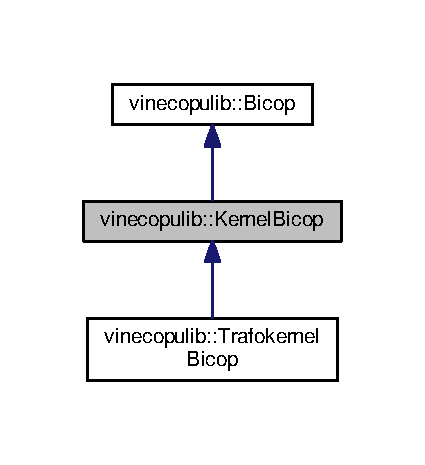
\includegraphics[width=213pt]{classvinecopulib_1_1_kernel_bicop__inherit__graph}
\end{center}
\end{figure}


Collaboration diagram for vinecopulib\+:\+:Kernel\+Bicop\+:
\nopagebreak
\begin{figure}[H]
\begin{center}
\leavevmode
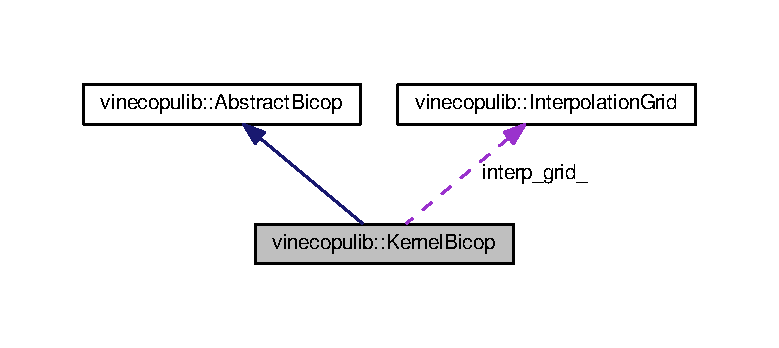
\includegraphics[width=350pt]{classvinecopulib_1_1_kernel_bicop__coll__graph}
\end{center}
\end{figure}
\subsection*{Protected Member Functions}
\begin{DoxyCompactItemize}
\item 
Eigen\+::\+Vector\+Xd {\bfseries pdf} (const Eigen\+::\+Matrix$<$ double, Eigen\+::\+Dynamic, 2 $>$ \&u)\hypertarget{classvinecopulib_1_1_kernel_bicop_a307624ad91ab1fd38ae7933fab0a5f6a}{}\label{classvinecopulib_1_1_kernel_bicop_a307624ad91ab1fd38ae7933fab0a5f6a}

\item 
Eigen\+::\+Vector\+Xd {\bfseries hfunc1} (const Eigen\+::\+Matrix$<$ double, Eigen\+::\+Dynamic, 2 $>$ \&u)\hypertarget{classvinecopulib_1_1_kernel_bicop_a08a6961d233bc977e583b5253c6089dc}{}\label{classvinecopulib_1_1_kernel_bicop_a08a6961d233bc977e583b5253c6089dc}

\item 
Eigen\+::\+Vector\+Xd {\bfseries hfunc2} (const Eigen\+::\+Matrix$<$ double, Eigen\+::\+Dynamic, 2 $>$ \&u)\hypertarget{classvinecopulib_1_1_kernel_bicop_ae4983795f404cca9c4a6af15d41b104a}{}\label{classvinecopulib_1_1_kernel_bicop_ae4983795f404cca9c4a6af15d41b104a}

\item 
Eigen\+::\+Vector\+Xd {\bfseries hinv1} (const Eigen\+::\+Matrix$<$ double, Eigen\+::\+Dynamic, 2 $>$ \&u)\hypertarget{classvinecopulib_1_1_kernel_bicop_aca726ccdf9a1551fb342dd7e60de1f84}{}\label{classvinecopulib_1_1_kernel_bicop_aca726ccdf9a1551fb342dd7e60de1f84}

\item 
Eigen\+::\+Vector\+Xd {\bfseries hinv2} (const Eigen\+::\+Matrix$<$ double, Eigen\+::\+Dynamic, 2 $>$ \&u)\hypertarget{classvinecopulib_1_1_kernel_bicop_a809dc2c7f0a67d217e0fe9651a625a6b}{}\label{classvinecopulib_1_1_kernel_bicop_a809dc2c7f0a67d217e0fe9651a625a6b}

\item 
double {\bfseries parameters\+\_\+to\+\_\+tau} (const Eigen\+::\+Vector\+Xd \&)\hypertarget{classvinecopulib_1_1_kernel_bicop_a1c00a74e12159b2c06487cf1b3ccff00}{}\label{classvinecopulib_1_1_kernel_bicop_a1c00a74e12159b2c06487cf1b3ccff00}

\item 
Eigen\+::\+Matrix\+Xd {\bfseries tau\+\_\+to\+\_\+parameters} (const double \&tau)\hypertarget{classvinecopulib_1_1_kernel_bicop_a510489f8f985c04c4f692e12ab2d1bf0}{}\label{classvinecopulib_1_1_kernel_bicop_a510489f8f985c04c4f692e12ab2d1bf0}

\item 
double {\bfseries calculate\+\_\+npars} ()\hypertarget{classvinecopulib_1_1_kernel_bicop_a33f736d5f443399f1f4dbe54b386aba3}{}\label{classvinecopulib_1_1_kernel_bicop_a33f736d5f443399f1f4dbe54b386aba3}

\item 
void {\bfseries flip} ()\hypertarget{classvinecopulib_1_1_kernel_bicop_abc23a81271f970b9c99dd6ed727c170f}{}\label{classvinecopulib_1_1_kernel_bicop_abc23a81271f970b9c99dd6ed727c170f}

\end{DoxyCompactItemize}
\subsection*{Protected Attributes}
\begin{DoxyCompactItemize}
\item 
\hyperlink{classvinecopulib_1_1_interpolation_grid}{Interpolation\+Grid} {\bfseries interp\+\_\+grid\+\_\+}\hypertarget{classvinecopulib_1_1_kernel_bicop_aa8cfe1dd0786d692562252de05c46588}{}\label{classvinecopulib_1_1_kernel_bicop_aa8cfe1dd0786d692562252de05c46588}

\item 
double {\bfseries npars\+\_\+}\hypertarget{classvinecopulib_1_1_kernel_bicop_a1b49a0a2630e71079c08ebdca79b06b6}{}\label{classvinecopulib_1_1_kernel_bicop_a1b49a0a2630e71079c08ebdca79b06b6}

\end{DoxyCompactItemize}
\subsection*{Additional Inherited Members}


\subsection{Detailed Description}
An abstract class for kernel copulas. 

Evaluation functions of kernel estimators are implemented efficiently using spline interpolation, see Nagler (2016).

This class is used in the implementation underlying the \hyperlink{classvinecopulib_1_1_bicop}{Bicop} class. Users should not use \hyperlink{classvinecopulib_1_1_abstract_bicop}{Abstract\+Bicop} or derived classes directly, but always work with the \hyperlink{classvinecopulib_1_1_bicop}{Bicop} interface.

Nagler, Thomas. {\itshape kdecopula\+: An R Package for the Kernel Estimation of Copula Densities}. ar\+Xiv\+:1603.\+04229 \mbox{[}stat.\+CO\mbox{]}, 2016 

The documentation for this class was generated from the following files\+:\begin{DoxyCompactItemize}
\item 
/home/n5/dev/cpp/vinecopulib/include/bicop/kernel.\+hpp\item 
/home/n5/dev/cpp/vinecopulib/src/bicop/kernel.\+cpp\end{DoxyCompactItemize}

\hypertarget{classvinecopulib_1_1tools__optimization_1_1_n_lopt_controls}{\section{vinecopulib\+:\+:tools\+\_\+optimization\+:\+:N\+Lopt\+Controls Class Reference}
\label{classvinecopulib_1_1tools__optimization_1_1_n_lopt_controls}\index{vinecopulib\+::tools\+\_\+optimization\+::\+N\+Lopt\+Controls@{vinecopulib\+::tools\+\_\+optimization\+::\+N\+Lopt\+Controls}}
}


A class for the controls to N\+Lopt.  




{\ttfamily \#include $<$tools\+\_\+optimization.\+hpp$>$}

\subsection*{Public Member Functions}
\begin{DoxyCompactItemize}
\item 
\hyperlink{classvinecopulib_1_1tools__optimization_1_1_n_lopt_controls_aaa09bb2bbf7dcbfcaaae4921b053c502}{N\+Lopt\+Controls} ()
\item 
\hyperlink{classvinecopulib_1_1tools__optimization_1_1_n_lopt_controls_aa8f12e7923d8dc5a28a49c6f23f204db}{N\+Lopt\+Controls} (double xtol\+\_\+rel, double xtol\+\_\+abs, double ftol\+\_\+rel, double ftol\+\_\+abs, int maxeval)
\end{DoxyCompactItemize}
\begin{Indent}{\bf Getters and setters}\par
\begin{DoxyCompactItemize}
\item 
void \hyperlink{classvinecopulib_1_1tools__optimization_1_1_n_lopt_controls_ab48d26a305e4ac805249605a60db4257}{set\+\_\+controls} (nlopt\+::opt $\ast$opt)
\item 
double \hyperlink{classvinecopulib_1_1tools__optimization_1_1_n_lopt_controls_a27400ff85f220911c2937ca16dd51697}{get\+\_\+xtol\+\_\+rel} ()
\item 
double \hyperlink{classvinecopulib_1_1tools__optimization_1_1_n_lopt_controls_a65494c81f12ff414259fd72593c545a6}{get\+\_\+xtol\+\_\+abs} ()
\item 
double \hyperlink{classvinecopulib_1_1tools__optimization_1_1_n_lopt_controls_a583ccb19e633f7408a1311aa250aabf7}{get\+\_\+ftol\+\_\+rel} ()
\item 
double \hyperlink{classvinecopulib_1_1tools__optimization_1_1_n_lopt_controls_ae96aba7bd7580c68216419722cafd3ec}{get\+\_\+ftol\+\_\+abs} ()
\item 
double \hyperlink{classvinecopulib_1_1tools__optimization_1_1_n_lopt_controls_a965d9632e85fae19778694bdfcbe1ea5}{get\+\_\+maxeval} ()
\end{DoxyCompactItemize}
\end{Indent}


\subsection{Detailed Description}
A class for the controls to N\+Lopt. 

\subsection{Constructor \& Destructor Documentation}
\hypertarget{classvinecopulib_1_1tools__optimization_1_1_n_lopt_controls_aaa09bb2bbf7dcbfcaaae4921b053c502}{\index{vinecopulib\+::tools\+\_\+optimization\+::\+N\+Lopt\+Controls@{vinecopulib\+::tools\+\_\+optimization\+::\+N\+Lopt\+Controls}!N\+Lopt\+Controls@{N\+Lopt\+Controls}}
\index{N\+Lopt\+Controls@{N\+Lopt\+Controls}!vinecopulib\+::tools\+\_\+optimization\+::\+N\+Lopt\+Controls@{vinecopulib\+::tools\+\_\+optimization\+::\+N\+Lopt\+Controls}}
\subsubsection[{N\+Lopt\+Controls}]{\setlength{\rightskip}{0pt plus 5cm}vinecopulib\+::tools\+\_\+optimization\+::\+N\+Lopt\+Controls\+::\+N\+Lopt\+Controls (
\begin{DoxyParamCaption}
{}
\end{DoxyParamCaption}
)}}\label{classvinecopulib_1_1tools__optimization_1_1_n_lopt_controls_aaa09bb2bbf7dcbfcaaae4921b053c502}
Create controls using the default contructor

The defaults are ``` xtol\+\_\+rel\+\_\+ = 1e-\/6; xtol\+\_\+abs\+\_\+ = 1e-\/6; ftol\+\_\+rel\+\_\+ = 1e-\/6; ftol\+\_\+abs\+\_\+ = 1e-\/6; maxeval\+\_\+ = 1000; ``` \hypertarget{classvinecopulib_1_1tools__optimization_1_1_n_lopt_controls_aa8f12e7923d8dc5a28a49c6f23f204db}{\index{vinecopulib\+::tools\+\_\+optimization\+::\+N\+Lopt\+Controls@{vinecopulib\+::tools\+\_\+optimization\+::\+N\+Lopt\+Controls}!N\+Lopt\+Controls@{N\+Lopt\+Controls}}
\index{N\+Lopt\+Controls@{N\+Lopt\+Controls}!vinecopulib\+::tools\+\_\+optimization\+::\+N\+Lopt\+Controls@{vinecopulib\+::tools\+\_\+optimization\+::\+N\+Lopt\+Controls}}
\subsubsection[{N\+Lopt\+Controls}]{\setlength{\rightskip}{0pt plus 5cm}vinecopulib\+::tools\+\_\+optimization\+::\+N\+Lopt\+Controls\+::\+N\+Lopt\+Controls (
\begin{DoxyParamCaption}
\item[{double}]{xtol\+\_\+rel, }
\item[{double}]{xtol\+\_\+abs, }
\item[{double}]{ftol\+\_\+rel, }
\item[{double}]{ftol\+\_\+abs, }
\item[{int}]{maxeval}
\end{DoxyParamCaption}
)}}\label{classvinecopulib_1_1tools__optimization_1_1_n_lopt_controls_aa8f12e7923d8dc5a28a49c6f23f204db}
Create controls by passing the arguments


\begin{DoxyParams}{Parameters}
{\em xtol\+\_\+rel} & relative tolerance on the parameter value. \\
\hline
{\em xtol\+\_\+abs} & absolute tolerance on the parameter value. \\
\hline
{\em ftol\+\_\+rel} & relative tolerance on the function value. \\
\hline
{\em ftol\+\_\+abs} & absolue tolerance on the function value. \\
\hline
{\em maxeval} & maximal number of evaluations of the objective. \\
\hline
\end{DoxyParams}


\subsection{Member Function Documentation}
\hypertarget{classvinecopulib_1_1tools__optimization_1_1_n_lopt_controls_ae96aba7bd7580c68216419722cafd3ec}{\index{vinecopulib\+::tools\+\_\+optimization\+::\+N\+Lopt\+Controls@{vinecopulib\+::tools\+\_\+optimization\+::\+N\+Lopt\+Controls}!get\+\_\+ftol\+\_\+abs@{get\+\_\+ftol\+\_\+abs}}
\index{get\+\_\+ftol\+\_\+abs@{get\+\_\+ftol\+\_\+abs}!vinecopulib\+::tools\+\_\+optimization\+::\+N\+Lopt\+Controls@{vinecopulib\+::tools\+\_\+optimization\+::\+N\+Lopt\+Controls}}
\subsubsection[{get\+\_\+ftol\+\_\+abs}]{\setlength{\rightskip}{0pt plus 5cm}double vinecopulib\+::tools\+\_\+optimization\+::\+N\+Lopt\+Controls\+::get\+\_\+ftol\+\_\+abs (
\begin{DoxyParamCaption}
{}
\end{DoxyParamCaption}
)}}\label{classvinecopulib_1_1tools__optimization_1_1_n_lopt_controls_ae96aba7bd7580c68216419722cafd3ec}
\begin{DoxyReturn}{Returns}
the absolute tolerance on the function value. 
\end{DoxyReturn}
\hypertarget{classvinecopulib_1_1tools__optimization_1_1_n_lopt_controls_a583ccb19e633f7408a1311aa250aabf7}{\index{vinecopulib\+::tools\+\_\+optimization\+::\+N\+Lopt\+Controls@{vinecopulib\+::tools\+\_\+optimization\+::\+N\+Lopt\+Controls}!get\+\_\+ftol\+\_\+rel@{get\+\_\+ftol\+\_\+rel}}
\index{get\+\_\+ftol\+\_\+rel@{get\+\_\+ftol\+\_\+rel}!vinecopulib\+::tools\+\_\+optimization\+::\+N\+Lopt\+Controls@{vinecopulib\+::tools\+\_\+optimization\+::\+N\+Lopt\+Controls}}
\subsubsection[{get\+\_\+ftol\+\_\+rel}]{\setlength{\rightskip}{0pt plus 5cm}double vinecopulib\+::tools\+\_\+optimization\+::\+N\+Lopt\+Controls\+::get\+\_\+ftol\+\_\+rel (
\begin{DoxyParamCaption}
{}
\end{DoxyParamCaption}
)}}\label{classvinecopulib_1_1tools__optimization_1_1_n_lopt_controls_a583ccb19e633f7408a1311aa250aabf7}
\begin{DoxyReturn}{Returns}
the relative tolerance on the function value. 
\end{DoxyReturn}
\hypertarget{classvinecopulib_1_1tools__optimization_1_1_n_lopt_controls_a965d9632e85fae19778694bdfcbe1ea5}{\index{vinecopulib\+::tools\+\_\+optimization\+::\+N\+Lopt\+Controls@{vinecopulib\+::tools\+\_\+optimization\+::\+N\+Lopt\+Controls}!get\+\_\+maxeval@{get\+\_\+maxeval}}
\index{get\+\_\+maxeval@{get\+\_\+maxeval}!vinecopulib\+::tools\+\_\+optimization\+::\+N\+Lopt\+Controls@{vinecopulib\+::tools\+\_\+optimization\+::\+N\+Lopt\+Controls}}
\subsubsection[{get\+\_\+maxeval}]{\setlength{\rightskip}{0pt plus 5cm}double vinecopulib\+::tools\+\_\+optimization\+::\+N\+Lopt\+Controls\+::get\+\_\+maxeval (
\begin{DoxyParamCaption}
{}
\end{DoxyParamCaption}
)}}\label{classvinecopulib_1_1tools__optimization_1_1_n_lopt_controls_a965d9632e85fae19778694bdfcbe1ea5}
\begin{DoxyReturn}{Returns}
the maximal number of evaluations of the objective. 
\end{DoxyReturn}
\hypertarget{classvinecopulib_1_1tools__optimization_1_1_n_lopt_controls_a65494c81f12ff414259fd72593c545a6}{\index{vinecopulib\+::tools\+\_\+optimization\+::\+N\+Lopt\+Controls@{vinecopulib\+::tools\+\_\+optimization\+::\+N\+Lopt\+Controls}!get\+\_\+xtol\+\_\+abs@{get\+\_\+xtol\+\_\+abs}}
\index{get\+\_\+xtol\+\_\+abs@{get\+\_\+xtol\+\_\+abs}!vinecopulib\+::tools\+\_\+optimization\+::\+N\+Lopt\+Controls@{vinecopulib\+::tools\+\_\+optimization\+::\+N\+Lopt\+Controls}}
\subsubsection[{get\+\_\+xtol\+\_\+abs}]{\setlength{\rightskip}{0pt plus 5cm}double vinecopulib\+::tools\+\_\+optimization\+::\+N\+Lopt\+Controls\+::get\+\_\+xtol\+\_\+abs (
\begin{DoxyParamCaption}
{}
\end{DoxyParamCaption}
)}}\label{classvinecopulib_1_1tools__optimization_1_1_n_lopt_controls_a65494c81f12ff414259fd72593c545a6}
\begin{DoxyReturn}{Returns}
the absolute tolerance on the parameter value. 
\end{DoxyReturn}
\hypertarget{classvinecopulib_1_1tools__optimization_1_1_n_lopt_controls_a27400ff85f220911c2937ca16dd51697}{\index{vinecopulib\+::tools\+\_\+optimization\+::\+N\+Lopt\+Controls@{vinecopulib\+::tools\+\_\+optimization\+::\+N\+Lopt\+Controls}!get\+\_\+xtol\+\_\+rel@{get\+\_\+xtol\+\_\+rel}}
\index{get\+\_\+xtol\+\_\+rel@{get\+\_\+xtol\+\_\+rel}!vinecopulib\+::tools\+\_\+optimization\+::\+N\+Lopt\+Controls@{vinecopulib\+::tools\+\_\+optimization\+::\+N\+Lopt\+Controls}}
\subsubsection[{get\+\_\+xtol\+\_\+rel}]{\setlength{\rightskip}{0pt plus 5cm}double vinecopulib\+::tools\+\_\+optimization\+::\+N\+Lopt\+Controls\+::get\+\_\+xtol\+\_\+rel (
\begin{DoxyParamCaption}
{}
\end{DoxyParamCaption}
)}}\label{classvinecopulib_1_1tools__optimization_1_1_n_lopt_controls_a27400ff85f220911c2937ca16dd51697}
\begin{DoxyReturn}{Returns}
the relative tolerance on the parameter value. 
\end{DoxyReturn}
\hypertarget{classvinecopulib_1_1tools__optimization_1_1_n_lopt_controls_ab48d26a305e4ac805249605a60db4257}{\index{vinecopulib\+::tools\+\_\+optimization\+::\+N\+Lopt\+Controls@{vinecopulib\+::tools\+\_\+optimization\+::\+N\+Lopt\+Controls}!set\+\_\+controls@{set\+\_\+controls}}
\index{set\+\_\+controls@{set\+\_\+controls}!vinecopulib\+::tools\+\_\+optimization\+::\+N\+Lopt\+Controls@{vinecopulib\+::tools\+\_\+optimization\+::\+N\+Lopt\+Controls}}
\subsubsection[{set\+\_\+controls}]{\setlength{\rightskip}{0pt plus 5cm}void vinecopulib\+::tools\+\_\+optimization\+::\+N\+Lopt\+Controls\+::set\+\_\+controls (
\begin{DoxyParamCaption}
\item[{nlopt\+::opt $\ast$}]{opt}
\end{DoxyParamCaption}
)}}\label{classvinecopulib_1_1tools__optimization_1_1_n_lopt_controls_ab48d26a305e4ac805249605a60db4257}
sets controls of an \hyperlink{classvinecopulib_1_1tools__optimization_1_1_optimizer}{Optimizer} 
\begin{DoxyParams}{Parameters}
{\em opt} & Pointer to the optimizer for control setting \\
\hline
\end{DoxyParams}


The documentation for this class was generated from the following files\+:\begin{DoxyCompactItemize}
\item 
vinecopulib/include/vinecopulib/misc/tools\+\_\+optimization.\+hpp\item 
vinecopulib/src/misc/tools\+\_\+optimization.\+cpp\end{DoxyCompactItemize}

\hypertarget{classvinecopulib_1_1tools__optimization_1_1_optimizer}{\section{vinecopulib\+:\+:tools\+\_\+optimization\+:\+:Optimizer Class Reference}
\label{classvinecopulib_1_1tools__optimization_1_1_optimizer}\index{vinecopulib\+::tools\+\_\+optimization\+::\+Optimizer@{vinecopulib\+::tools\+\_\+optimization\+::\+Optimizer}}
}


A class for optimization (wrapping N\+Lopt).  




{\ttfamily \#include $<$tools\+\_\+optimization.\+hpp$>$}

\subsection*{Public Member Functions}
\begin{DoxyCompactItemize}
\item 
\hyperlink{classvinecopulib_1_1tools__optimization_1_1_optimizer_a1514592e4adccdcc544bb32654e81da1}{Optimizer} (unsigned int n\+\_\+parameters)
\item 
\hyperlink{classvinecopulib_1_1tools__optimization_1_1_optimizer_a43190e80f015257e203c134826857c7c}{Optimizer} (unsigned int n\+\_\+parameters, double xtol\+\_\+rel, double xtol\+\_\+abs, double ftol\+\_\+rel, double ftol\+\_\+abs, int maxeval)
\item 
void \hyperlink{classvinecopulib_1_1tools__optimization_1_1_optimizer_a907419eedf3bb18766d2cb7340a06f7d}{set\+\_\+bounds} (const Eigen\+::\+Matrix\+Xd \&lower\+\_\+bounds, const Eigen\+::\+Matrix\+Xd \&upper\+\_\+bounds)
\item 
void \hyperlink{classvinecopulib_1_1tools__optimization_1_1_optimizer_a14495a0b3219e176fce553beb4a643b9}{set\+\_\+objective} (nlopt\+::vfunc f, void $\ast$f\+\_\+data)
\item 
Eigen\+::\+Vector\+Xd \hyperlink{classvinecopulib_1_1tools__optimization_1_1_optimizer_a3c4fcd7a4d3a792d2a9e57349f271764}{optimize} (Eigen\+::\+Vector\+Xd initial\+\_\+parameters)
\end{DoxyCompactItemize}


\subsection{Detailed Description}
A class for optimization (wrapping N\+Lopt). 

\subsection{Constructor \& Destructor Documentation}
\hypertarget{classvinecopulib_1_1tools__optimization_1_1_optimizer_a1514592e4adccdcc544bb32654e81da1}{\index{vinecopulib\+::tools\+\_\+optimization\+::\+Optimizer@{vinecopulib\+::tools\+\_\+optimization\+::\+Optimizer}!Optimizer@{Optimizer}}
\index{Optimizer@{Optimizer}!vinecopulib\+::tools\+\_\+optimization\+::\+Optimizer@{vinecopulib\+::tools\+\_\+optimization\+::\+Optimizer}}
\subsubsection[{Optimizer}]{\setlength{\rightskip}{0pt plus 5cm}vinecopulib\+::tools\+\_\+optimization\+::\+Optimizer\+::\+Optimizer (
\begin{DoxyParamCaption}
\item[{unsigned int}]{n\+\_\+parameters}
\end{DoxyParamCaption}
)}}\label{classvinecopulib_1_1tools__optimization_1_1_optimizer_a1514592e4adccdcc544bb32654e81da1}
creates an \hyperlink{classvinecopulib_1_1tools__optimization_1_1_optimizer}{Optimizer} using the default controls, see \hyperlink{classvinecopulib_1_1tools__optimization_1_1_n_lopt_controls}{N\+Lopt\+Controls}.


\begin{DoxyParams}{Parameters}
{\em n\+\_\+parameters} & Number of parameters to optimize \\
\hline
\end{DoxyParams}
\hypertarget{classvinecopulib_1_1tools__optimization_1_1_optimizer_a43190e80f015257e203c134826857c7c}{\index{vinecopulib\+::tools\+\_\+optimization\+::\+Optimizer@{vinecopulib\+::tools\+\_\+optimization\+::\+Optimizer}!Optimizer@{Optimizer}}
\index{Optimizer@{Optimizer}!vinecopulib\+::tools\+\_\+optimization\+::\+Optimizer@{vinecopulib\+::tools\+\_\+optimization\+::\+Optimizer}}
\subsubsection[{Optimizer}]{\setlength{\rightskip}{0pt plus 5cm}vinecopulib\+::tools\+\_\+optimization\+::\+Optimizer\+::\+Optimizer (
\begin{DoxyParamCaption}
\item[{unsigned int}]{n\+\_\+parameters, }
\item[{double}]{xtol\+\_\+rel, }
\item[{double}]{xtol\+\_\+abs, }
\item[{double}]{ftol\+\_\+rel, }
\item[{double}]{ftol\+\_\+abs, }
\item[{int}]{maxeval}
\end{DoxyParamCaption}
)}}\label{classvinecopulib_1_1tools__optimization_1_1_optimizer_a43190e80f015257e203c134826857c7c}
creates an optimizer using custom controls.


\begin{DoxyParams}{Parameters}
{\em n\+\_\+parameters} & number of parameters to optimize. \\
\hline
{\em xtol\+\_\+rel} & relative tolerance on the parameter value. \\
\hline
{\em xtol\+\_\+abs} & absolute tolerance on the parameter value. \\
\hline
{\em ftol\+\_\+rel} & relative tolerance on the function value. \\
\hline
{\em ftol\+\_\+abs} & absolue tolerance on the function value. \\
\hline
{\em maxeval} & maximal number of evaluations of the objective. \\
\hline
\end{DoxyParams}


\subsection{Member Function Documentation}
\hypertarget{classvinecopulib_1_1tools__optimization_1_1_optimizer_a3c4fcd7a4d3a792d2a9e57349f271764}{\index{vinecopulib\+::tools\+\_\+optimization\+::\+Optimizer@{vinecopulib\+::tools\+\_\+optimization\+::\+Optimizer}!optimize@{optimize}}
\index{optimize@{optimize}!vinecopulib\+::tools\+\_\+optimization\+::\+Optimizer@{vinecopulib\+::tools\+\_\+optimization\+::\+Optimizer}}
\subsubsection[{optimize}]{\setlength{\rightskip}{0pt plus 5cm}Eigen\+::\+Vector\+Xd vinecopulib\+::tools\+\_\+optimization\+::\+Optimizer\+::optimize (
\begin{DoxyParamCaption}
\item[{Eigen\+::\+Vector\+Xd}]{initial\+\_\+parameters}
\end{DoxyParamCaption}
)}}\label{classvinecopulib_1_1tools__optimization_1_1_optimizer_a3c4fcd7a4d3a792d2a9e57349f271764}
solve the optimization problem.


\begin{DoxyParams}{Parameters}
{\em initial\+\_\+parameters} & of starting values for the optimization algorithm. \\
\hline
\end{DoxyParams}
\begin{DoxyReturn}{Returns}
the optimal parameters. 
\end{DoxyReturn}
\hypertarget{classvinecopulib_1_1tools__optimization_1_1_optimizer_a907419eedf3bb18766d2cb7340a06f7d}{\index{vinecopulib\+::tools\+\_\+optimization\+::\+Optimizer@{vinecopulib\+::tools\+\_\+optimization\+::\+Optimizer}!set\+\_\+bounds@{set\+\_\+bounds}}
\index{set\+\_\+bounds@{set\+\_\+bounds}!vinecopulib\+::tools\+\_\+optimization\+::\+Optimizer@{vinecopulib\+::tools\+\_\+optimization\+::\+Optimizer}}
\subsubsection[{set\+\_\+bounds}]{\setlength{\rightskip}{0pt plus 5cm}void vinecopulib\+::tools\+\_\+optimization\+::\+Optimizer\+::set\+\_\+bounds (
\begin{DoxyParamCaption}
\item[{const Eigen\+::\+Matrix\+Xd \&}]{lower\+\_\+bounds, }
\item[{const Eigen\+::\+Matrix\+Xd \&}]{upper\+\_\+bounds}
\end{DoxyParamCaption}
)}}\label{classvinecopulib_1_1tools__optimization_1_1_optimizer_a907419eedf3bb18766d2cb7340a06f7d}
sets the optimizer's bounds. 
\begin{DoxyParams}{Parameters}
{\em lower\+\_\+bounds} & \\
\hline
{\em upper\+\_\+bounds} & \\
\hline
\end{DoxyParams}
\hypertarget{classvinecopulib_1_1tools__optimization_1_1_optimizer_a14495a0b3219e176fce553beb4a643b9}{\index{vinecopulib\+::tools\+\_\+optimization\+::\+Optimizer@{vinecopulib\+::tools\+\_\+optimization\+::\+Optimizer}!set\+\_\+objective@{set\+\_\+objective}}
\index{set\+\_\+objective@{set\+\_\+objective}!vinecopulib\+::tools\+\_\+optimization\+::\+Optimizer@{vinecopulib\+::tools\+\_\+optimization\+::\+Optimizer}}
\subsubsection[{set\+\_\+objective}]{\setlength{\rightskip}{0pt plus 5cm}void vinecopulib\+::tools\+\_\+optimization\+::\+Optimizer\+::set\+\_\+objective (
\begin{DoxyParamCaption}
\item[{nlopt\+::vfunc}]{f, }
\item[{void $\ast$}]{f\+\_\+data}
\end{DoxyParamCaption}
)}}\label{classvinecopulib_1_1tools__optimization_1_1_optimizer_a14495a0b3219e176fce553beb4a643b9}
Set the optimizer's objective and data


\begin{DoxyParams}{Parameters}
{\em f} & The optimizer's objective function (see nlopt's documentation) \\
\hline
{\em f\+\_\+data} & The optimizer's data (see nlopt's documentation) \\
\hline
\end{DoxyParams}


The documentation for this class was generated from the following files\+:\begin{DoxyCompactItemize}
\item 
vinecopulib/include/vinecopulib/misc/tools\+\_\+optimization.\+hpp\item 
vinecopulib/src/misc/tools\+\_\+optimization.\+cpp\end{DoxyCompactItemize}

\hypertarget{classvinecopulib_1_1_par_bicop}{}\section{vinecopulib\+:\+:Par\+Bicop Class Reference}
\label{classvinecopulib_1_1_par_bicop}\index{vinecopulib\+::\+Par\+Bicop@{vinecopulib\+::\+Par\+Bicop}}


Inheritance diagram for vinecopulib\+:\+:Par\+Bicop\+:\nopagebreak
\begin{figure}[H]
\begin{center}
\leavevmode
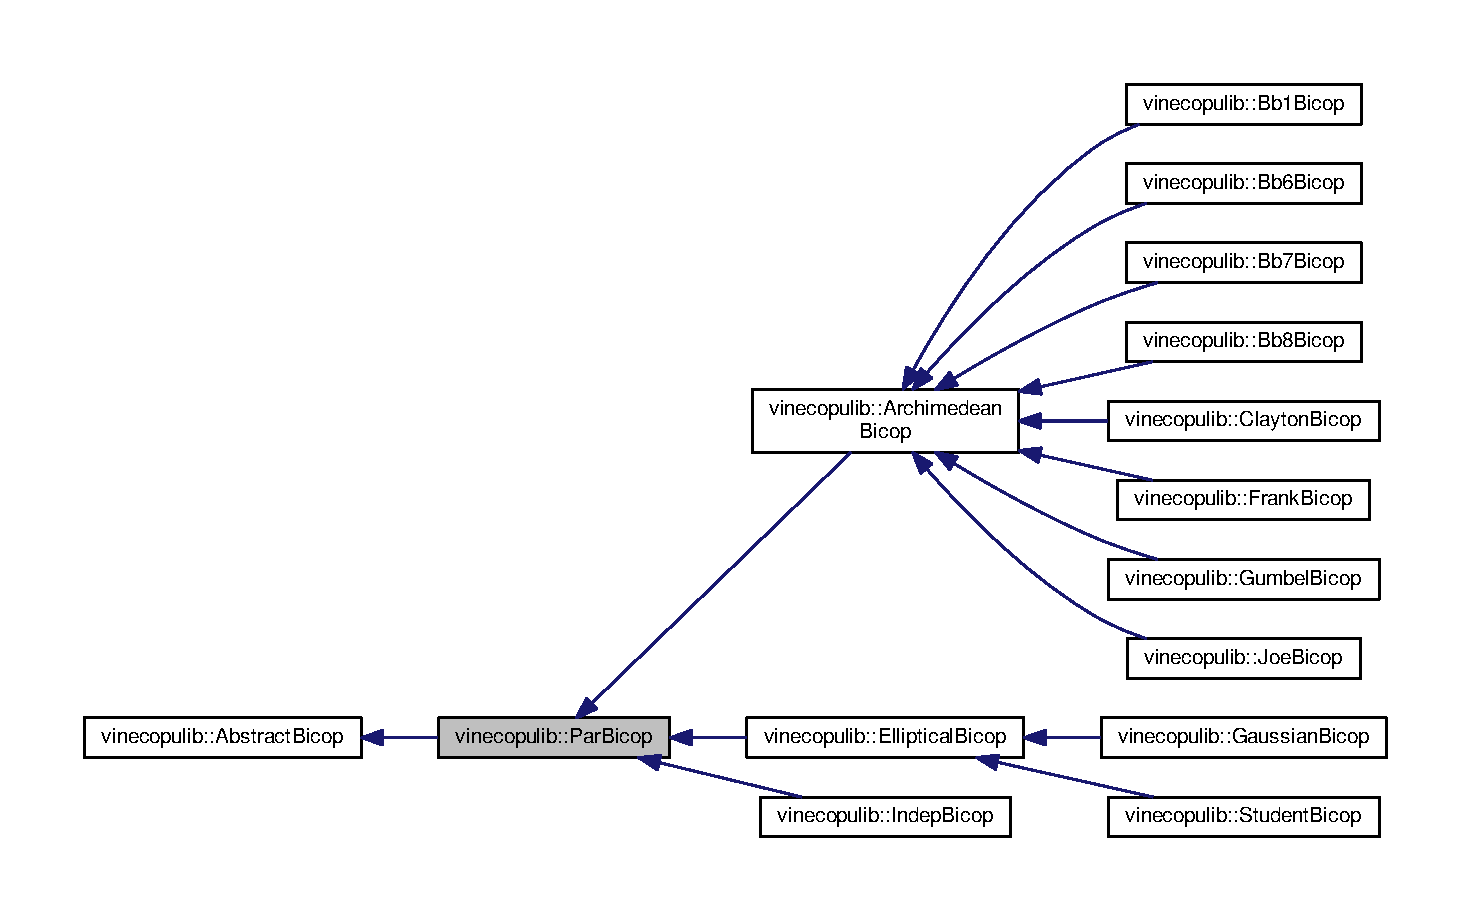
\includegraphics[width=350pt]{classvinecopulib_1_1_par_bicop__inherit__graph}
\end{center}
\end{figure}


Collaboration diagram for vinecopulib\+:\+:Par\+Bicop\+:\nopagebreak
\begin{figure}[H]
\begin{center}
\leavevmode
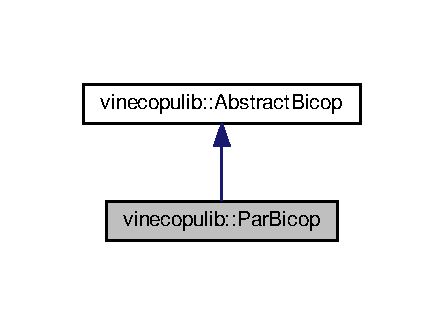
\includegraphics[width=191pt]{classvinecopulib_1_1_par_bicop__coll__graph}
\end{center}
\end{figure}
\subsection*{Additional Inherited Members}


The documentation for this class was generated from the following files\+:\begin{DoxyCompactItemize}
\item 
/home/n5/dev/cpp/vinecopulib/include/bicop\+\_\+parametric.\+hpp\item 
/home/n5/dev/cpp/vinecopulib/src/bicop\+\_\+parametric.\+cpp\end{DoxyCompactItemize}

\hypertarget{structvinecopulib_1_1tools__optimization_1_1_par_bicop_opt_data}{\section{vinecopulib\+:\+:tools\+\_\+optimization\+:\+:Par\+Bicop\+Opt\+Data Struct Reference}
\label{structvinecopulib_1_1tools__optimization_1_1_par_bicop_opt_data}\index{vinecopulib\+::tools\+\_\+optimization\+::\+Par\+Bicop\+Opt\+Data@{vinecopulib\+::tools\+\_\+optimization\+::\+Par\+Bicop\+Opt\+Data}}
}


A helper struct for (profile) maximum likelihood estimation.  




{\ttfamily \#include $<$tools\+\_\+optimization.\+hpp$>$}



Collaboration diagram for vinecopulib\+:\+:tools\+\_\+optimization\+:\+:Par\+Bicop\+Opt\+Data\+:\nopagebreak
\begin{figure}[H]
\begin{center}
\leavevmode
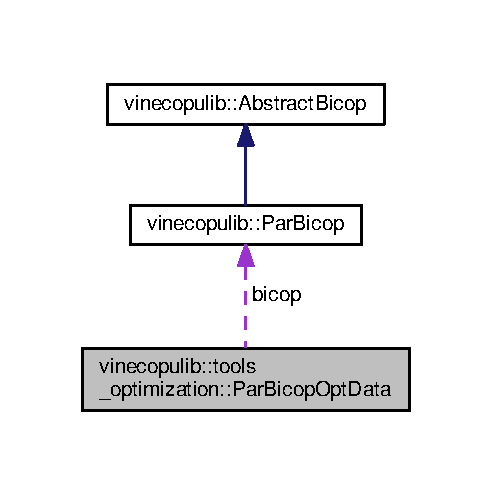
\includegraphics[width=236pt]{structvinecopulib_1_1tools__optimization_1_1_par_bicop_opt_data__coll__graph}
\end{center}
\end{figure}
\subsection*{Public Attributes}
\begin{DoxyCompactItemize}
\item 
\hypertarget{structvinecopulib_1_1tools__optimization_1_1_par_bicop_opt_data_ad5c1e327926fbbe10a20d65c7bf7b85a}{const Eigen\+::\+Matrix$<$ double, \\*
Eigen\+::\+Dynamic, 2 $>$ \& \hyperlink{structvinecopulib_1_1tools__optimization_1_1_par_bicop_opt_data_ad5c1e327926fbbe10a20d65c7bf7b85a}{U}}\label{structvinecopulib_1_1tools__optimization_1_1_par_bicop_opt_data_ad5c1e327926fbbe10a20d65c7bf7b85a}

\begin{DoxyCompactList}\small\item\em the data. \end{DoxyCompactList}\item 
\hypertarget{structvinecopulib_1_1tools__optimization_1_1_par_bicop_opt_data_a8ead6cc4ff570a56214de4036b3149b4}{\hyperlink{classvinecopulib_1_1_par_bicop}{vinecopulib\+::\+Par\+Bicop} $\ast$ \hyperlink{structvinecopulib_1_1tools__optimization_1_1_par_bicop_opt_data_a8ead6cc4ff570a56214de4036b3149b4}{bicop}}\label{structvinecopulib_1_1tools__optimization_1_1_par_bicop_opt_data_a8ead6cc4ff570a56214de4036b3149b4}

\begin{DoxyCompactList}\small\item\em a pointer to the bivariate copula to optimize. \end{DoxyCompactList}\item 
\hypertarget{structvinecopulib_1_1tools__optimization_1_1_par_bicop_opt_data_a9991ee2b06cc43912d620a0ac07b3de9}{double \hyperlink{structvinecopulib_1_1tools__optimization_1_1_par_bicop_opt_data_a9991ee2b06cc43912d620a0ac07b3de9}{par0}}\label{structvinecopulib_1_1tools__optimization_1_1_par_bicop_opt_data_a9991ee2b06cc43912d620a0ac07b3de9}

\begin{DoxyCompactList}\small\item\em main dependence parameter. \end{DoxyCompactList}\item 
\hypertarget{structvinecopulib_1_1tools__optimization_1_1_par_bicop_opt_data_adfc58183f8a6074fdf5a0e7d0bbc0cd9}{unsigned int \hyperlink{structvinecopulib_1_1tools__optimization_1_1_par_bicop_opt_data_adfc58183f8a6074fdf5a0e7d0bbc0cd9}{objective\+\_\+calls}}\label{structvinecopulib_1_1tools__optimization_1_1_par_bicop_opt_data_adfc58183f8a6074fdf5a0e7d0bbc0cd9}

\begin{DoxyCompactList}\small\item\em number of evaluations of the objective. \end{DoxyCompactList}\end{DoxyCompactItemize}


\subsection{Detailed Description}
A helper struct for (profile) maximum likelihood estimation. 

The documentation for this struct was generated from the following file\+:\begin{DoxyCompactItemize}
\item 
vinecopulib/include/vinecopulib/misc/tools\+\_\+optimization.\+hpp\end{DoxyCompactItemize}

\hypertarget{classvinecopulib_1_1_r_vine_matrix}{\section{vinecopulib\+:\+:R\+Vine\+Matrix Class Reference}
\label{classvinecopulib_1_1_r_vine_matrix}\index{vinecopulib\+::\+R\+Vine\+Matrix@{vinecopulib\+::\+R\+Vine\+Matrix}}
}


A class for regular vine matrices.  




{\ttfamily \#include $<$rvine\+\_\+matrix.\+hpp$>$}

\subsection*{Public Member Functions}
\begin{DoxyCompactItemize}
\item 
\hyperlink{classvinecopulib_1_1_r_vine_matrix_a966316e211937ae11e840ef7540a492f}{R\+Vine\+Matrix} (const Eigen\+::\+Matrix$<$ size\+\_\+t, Eigen\+::\+Dynamic, Eigen\+::\+Dynamic $>$ \&matrix, bool check=true)
\item 
\hypertarget{classvinecopulib_1_1_r_vine_matrix_a37c79233fca1e56e1535cbb37f8d3177}{Eigen\+::\+Matrix$<$ size\+\_\+t, \\*
Eigen\+::\+Dynamic, Eigen\+::\+Dynamic $>$ \hyperlink{classvinecopulib_1_1_r_vine_matrix_a37c79233fca1e56e1535cbb37f8d3177}{get\+\_\+matrix} () const }\label{classvinecopulib_1_1_r_vine_matrix_a37c79233fca1e56e1535cbb37f8d3177}

\begin{DoxyCompactList}\small\item\em extract the matrix. \end{DoxyCompactList}\item 
\hypertarget{classvinecopulib_1_1_r_vine_matrix_a71554c734c3cbb4c066c1f17fe94a284}{Eigen\+::\+Matrix$<$ size\+\_\+t, \\*
Eigen\+::\+Dynamic, 1 $>$ \hyperlink{classvinecopulib_1_1_r_vine_matrix_a71554c734c3cbb4c066c1f17fe94a284}{get\+\_\+order} () const }\label{classvinecopulib_1_1_r_vine_matrix_a71554c734c3cbb4c066c1f17fe94a284}

\begin{DoxyCompactList}\small\item\em extracts the variable order in the R-\/vine. \end{DoxyCompactList}\item 
Eigen\+::\+Matrix$<$ size\+\_\+t, \\*
Eigen\+::\+Dynamic, Eigen\+::\+Dynamic $>$ \hyperlink{classvinecopulib_1_1_r_vine_matrix_a4e63d8b01e1d89284ca28192676b8a3f}{in\+\_\+natural\+\_\+order} () const 
\item 
Eigen\+::\+Matrix$<$ size\+\_\+t, \\*
Eigen\+::\+Dynamic, Eigen\+::\+Dynamic $>$ \hyperlink{classvinecopulib_1_1_r_vine_matrix_aef8bbe14451d023e1c9c113e3812f574}{get\+\_\+max\+\_\+matrix} () const 
\item 
\hyperlink{namespacevinecopulib_1_1tools__eigen_a2fcd63009df35741859f44f1e41931f9}{Matrix\+Xb} \hyperlink{classvinecopulib_1_1_r_vine_matrix_a6303fc1f643fdf793c867ca7e08e42bc}{get\+\_\+needed\+\_\+hfunc1} () const 
\item 
\hyperlink{namespacevinecopulib_1_1tools__eigen_a2fcd63009df35741859f44f1e41931f9}{Matrix\+Xb} \hyperlink{classvinecopulib_1_1_r_vine_matrix_a7ac32cf10a966ba567142e9b36106746}{get\+\_\+needed\+\_\+hfunc2} () const 
\end{DoxyCompactItemize}
\subsection*{Static Public Member Functions}
\begin{DoxyCompactItemize}
\item 
static Eigen\+::\+Matrix$<$ size\+\_\+t, \\*
Eigen\+::\+Dynamic, Eigen\+::\+Dynamic $>$ \hyperlink{classvinecopulib_1_1_r_vine_matrix_ad523b84e2ea41eba4eb982eb9b39471b}{construct\+\_\+d\+\_\+vine\+\_\+matrix} (const Eigen\+::\+Matrix$<$ size\+\_\+t, Eigen\+::\+Dynamic, 1 $>$ \&order)
\end{DoxyCompactItemize}


\subsection{Detailed Description}
A class for regular vine matrices. 

A regular vine (R-\/vine) matrix encodes the structure of a vine. An examplary matrix is ``` 1 1 1 1 2 2 2 0 3 3 0 0 4 0 0 0 ``` which encodes the following pair-\/copulas\+: ``` \begin{TabularC}{3}
\hline
\rowcolor{lightgray}{\bf tree }&{\bf edge }&{\bf pair-\/copulas  }\\\cline{1-3}
0 &0 &{\ttfamily (4, 1)} \\\cline{1-3}
&1 &{\ttfamily (3, 1)} \\\cline{1-3}
&2 &{\ttfamily (2, 1)} \\\cline{1-3}
1 &0 &{\ttfamily (4, 2; 1)} \\\cline{1-3}
&1 &{\ttfamily (3, 2; 1)} \\\cline{1-3}
2 &0 &{\ttfamily (4, 3; 2, 1)} \\\cline{1-3}
\end{TabularC}
``{\ttfamily  Denoting by}M\mbox{[}i\mbox{]}\mbox{[}j\mbox{]}{\ttfamily the matrix entry in row}i{\ttfamily and column}j{\ttfamily  (starting at 0), the pair-\/copula index for edge}e{\ttfamily in tree}t{\ttfamily of a }d{\ttfamily dimensional vine is }(M\mbox{[}d -\/ 1 -\/ t\mbox{]}\mbox{[}e\mbox{]}, M\mbox{[}t\mbox{]}\mbox{[}e\mbox{]}; M\mbox{[}t -\/ 1\mbox{]}\mbox{[}e\mbox{]}, ..., M\mbox{[}0\mbox{]}\mbox{[}e\mbox{]})`. Less formally,
\begin{DoxyEnumerate}
\item Start with the counter-\/diagonal element of column {\ttfamily e} (first conditioned variable).
\item Jump up to the element in row {\ttfamily t} (second conditioned variable).
\item Gather all entries further up in column {\ttfamily e} (conditioning set).
\end{DoxyEnumerate}

A valid R-\/vine matrix must satisfy several conditions which are checked when {\ttfamily R\+Vine\+Matrix()} is called\+:
\begin{DoxyEnumerate}
\item The lower right triangle must only contain zeros.
\item The upper left triangle can only contain numbers between 1 and d.
\item The antidiagonal must contain the numbers 1, ..., d.
\item The antidiagonal entry of a column must not be contained in any column further to the right.
\item The entries of a column must be contained in all columns to the left.
\item The proximity condition must hold\+: For all t = 1, ..., d -\/ 2 and e = 0, ..., d -\/ t -\/ 1 there must exist an index j $>$ d, such that {\ttfamily (M\mbox{[}t, e\mbox{]}, \{M\mbox{[}0, e\mbox{]}, ..., M\mbox{[}t-\/1, e\mbox{]}\})} equals either {\ttfamily (M\mbox{[}d-\/j-\/1, j\mbox{]}, \{M\mbox{[}0, j\mbox{]}, ..., M\mbox{[}t-\/1, j\mbox{]}\})} or {\ttfamily (M\mbox{[}t-\/1, j\mbox{]}, \{M\mbox{[}d-\/j-\/1, j\mbox{]}, M\mbox{[}0, j\mbox{]}, ..., M\mbox{[}t-\/2, j\mbox{]}\})}.
\end{DoxyEnumerate}

Condition 6 already implies conditions 2-\/5, but is more difficult to check by hand. 

\subsection{Constructor \& Destructor Documentation}
\hypertarget{classvinecopulib_1_1_r_vine_matrix_a966316e211937ae11e840ef7540a492f}{\index{vinecopulib\+::\+R\+Vine\+Matrix@{vinecopulib\+::\+R\+Vine\+Matrix}!R\+Vine\+Matrix@{R\+Vine\+Matrix}}
\index{R\+Vine\+Matrix@{R\+Vine\+Matrix}!vinecopulib\+::\+R\+Vine\+Matrix@{vinecopulib\+::\+R\+Vine\+Matrix}}
\subsubsection[{R\+Vine\+Matrix}]{\setlength{\rightskip}{0pt plus 5cm}vinecopulib\+::\+R\+Vine\+Matrix\+::\+R\+Vine\+Matrix (
\begin{DoxyParamCaption}
\item[{const Eigen\+::\+Matrix$<$ size\+\_\+t, Eigen\+::\+Dynamic, Eigen\+::\+Dynamic $>$ \&}]{matrix, }
\item[{bool}]{check = {\ttfamily true}}
\end{DoxyParamCaption}
)}}\label{classvinecopulib_1_1_r_vine_matrix_a966316e211937ae11e840ef7540a492f}
instantiates an \hyperlink{classvinecopulib_1_1_r_vine_matrix}{R\+Vine\+Matrix} object. 
\begin{DoxyParams}{Parameters}
{\em matrix} & a valid R-\/vine matrix. \\
\hline
{\em check} & whether the matrix shall be checked for validity. \\
\hline
\end{DoxyParams}


\subsection{Member Function Documentation}
\hypertarget{classvinecopulib_1_1_r_vine_matrix_ad523b84e2ea41eba4eb982eb9b39471b}{\index{vinecopulib\+::\+R\+Vine\+Matrix@{vinecopulib\+::\+R\+Vine\+Matrix}!construct\+\_\+d\+\_\+vine\+\_\+matrix@{construct\+\_\+d\+\_\+vine\+\_\+matrix}}
\index{construct\+\_\+d\+\_\+vine\+\_\+matrix@{construct\+\_\+d\+\_\+vine\+\_\+matrix}!vinecopulib\+::\+R\+Vine\+Matrix@{vinecopulib\+::\+R\+Vine\+Matrix}}
\subsubsection[{construct\+\_\+d\+\_\+vine\+\_\+matrix}]{\setlength{\rightskip}{0pt plus 5cm}Eigen\+::\+Matrix$<$ size\+\_\+t, Eigen\+::\+Dynamic, Eigen\+::\+Dynamic $>$ vinecopulib\+::\+R\+Vine\+Matrix\+::construct\+\_\+d\+\_\+vine\+\_\+matrix (
\begin{DoxyParamCaption}
\item[{const Eigen\+::\+Matrix$<$ size\+\_\+t, Eigen\+::\+Dynamic, 1 $>$ \&}]{order}
\end{DoxyParamCaption}
)\hspace{0.3cm}{\ttfamily [static]}}}\label{classvinecopulib_1_1_r_vine_matrix_ad523b84e2ea41eba4eb982eb9b39471b}
constructs a D-\/vine matrix.

A D-\/vine is a vine where each tree is a path.


\begin{DoxyParams}{Parameters}
{\em order} & order of the variables. \\
\hline
\end{DoxyParams}
\hypertarget{classvinecopulib_1_1_r_vine_matrix_aef8bbe14451d023e1c9c113e3812f574}{\index{vinecopulib\+::\+R\+Vine\+Matrix@{vinecopulib\+::\+R\+Vine\+Matrix}!get\+\_\+max\+\_\+matrix@{get\+\_\+max\+\_\+matrix}}
\index{get\+\_\+max\+\_\+matrix@{get\+\_\+max\+\_\+matrix}!vinecopulib\+::\+R\+Vine\+Matrix@{vinecopulib\+::\+R\+Vine\+Matrix}}
\subsubsection[{get\+\_\+max\+\_\+matrix}]{\setlength{\rightskip}{0pt plus 5cm}Eigen\+::\+Matrix$<$ size\+\_\+t, Eigen\+::\+Dynamic, Eigen\+::\+Dynamic $>$ vinecopulib\+::\+R\+Vine\+Matrix\+::get\+\_\+max\+\_\+matrix (
\begin{DoxyParamCaption}
{}
\end{DoxyParamCaption}
) const}}\label{classvinecopulib_1_1_r_vine_matrix_aef8bbe14451d023e1c9c113e3812f574}
extracts the maximum matrix.

The maximum matrix is derived from an R-\/vine matrix by iteratively computing the (elementwise) maximum of a row and the row below (starting from the bottom). It is used in estimation and evaluation algorithms to find the right pseudo observations for an edge. \hypertarget{classvinecopulib_1_1_r_vine_matrix_a6303fc1f643fdf793c867ca7e08e42bc}{\index{vinecopulib\+::\+R\+Vine\+Matrix@{vinecopulib\+::\+R\+Vine\+Matrix}!get\+\_\+needed\+\_\+hfunc1@{get\+\_\+needed\+\_\+hfunc1}}
\index{get\+\_\+needed\+\_\+hfunc1@{get\+\_\+needed\+\_\+hfunc1}!vinecopulib\+::\+R\+Vine\+Matrix@{vinecopulib\+::\+R\+Vine\+Matrix}}
\subsubsection[{get\+\_\+needed\+\_\+hfunc1}]{\setlength{\rightskip}{0pt plus 5cm}{\bf Matrix\+Xb} vinecopulib\+::\+R\+Vine\+Matrix\+::get\+\_\+needed\+\_\+hfunc1 (
\begin{DoxyParamCaption}
{}
\end{DoxyParamCaption}
) const}}\label{classvinecopulib_1_1_r_vine_matrix_a6303fc1f643fdf793c867ca7e08e42bc}
extracts a matrix indicating which of the first h-\/functions are needed (it is usually not necessary to apply both h-\/functions for each pair-\/copula). \hypertarget{classvinecopulib_1_1_r_vine_matrix_a7ac32cf10a966ba567142e9b36106746}{\index{vinecopulib\+::\+R\+Vine\+Matrix@{vinecopulib\+::\+R\+Vine\+Matrix}!get\+\_\+needed\+\_\+hfunc2@{get\+\_\+needed\+\_\+hfunc2}}
\index{get\+\_\+needed\+\_\+hfunc2@{get\+\_\+needed\+\_\+hfunc2}!vinecopulib\+::\+R\+Vine\+Matrix@{vinecopulib\+::\+R\+Vine\+Matrix}}
\subsubsection[{get\+\_\+needed\+\_\+hfunc2}]{\setlength{\rightskip}{0pt plus 5cm}{\bf Matrix\+Xb} vinecopulib\+::\+R\+Vine\+Matrix\+::get\+\_\+needed\+\_\+hfunc2 (
\begin{DoxyParamCaption}
{}
\end{DoxyParamCaption}
) const}}\label{classvinecopulib_1_1_r_vine_matrix_a7ac32cf10a966ba567142e9b36106746}
extracts a matrix indicating which of the second h-\/functions are needed (it is usually not necessary to apply both h-\/functions for each pair-\/copula). \hypertarget{classvinecopulib_1_1_r_vine_matrix_a4e63d8b01e1d89284ca28192676b8a3f}{\index{vinecopulib\+::\+R\+Vine\+Matrix@{vinecopulib\+::\+R\+Vine\+Matrix}!in\+\_\+natural\+\_\+order@{in\+\_\+natural\+\_\+order}}
\index{in\+\_\+natural\+\_\+order@{in\+\_\+natural\+\_\+order}!vinecopulib\+::\+R\+Vine\+Matrix@{vinecopulib\+::\+R\+Vine\+Matrix}}
\subsubsection[{in\+\_\+natural\+\_\+order}]{\setlength{\rightskip}{0pt plus 5cm}Eigen\+::\+Matrix$<$ size\+\_\+t, Eigen\+::\+Dynamic, Eigen\+::\+Dynamic $>$ vinecopulib\+::\+R\+Vine\+Matrix\+::in\+\_\+natural\+\_\+order (
\begin{DoxyParamCaption}
{}
\end{DoxyParamCaption}
) const}}\label{classvinecopulib_1_1_r_vine_matrix_a4e63d8b01e1d89284ca28192676b8a3f}
extracts the R-\/vine matrix in natural order.

Natural order means that the counter-\/diagonal has entries (d, ..., 1). We convert to natural order by relabeling the variables. Most algorithms for estimation and evaluation assume that the R-\/vine matrix is in natural order. 

The documentation for this class was generated from the following files\+:\begin{DoxyCompactItemize}
\item 
vinecopulib/include/vinecopulib/vinecop/rvine\+\_\+matrix.\+hpp\item 
vinecopulib/src/vinecop/rvine\+\_\+matrix.\+cpp\end{DoxyCompactItemize}

\hypertarget{classvinecopulib_1_1_student_bicop}{\section{vinecopulib\+:\+:Student\+Bicop Class Reference}
\label{classvinecopulib_1_1_student_bicop}\index{vinecopulib\+::\+Student\+Bicop@{vinecopulib\+::\+Student\+Bicop}}
}


The Student t copula.  




{\ttfamily \#include $<$student.\+hpp$>$}



Inheritance diagram for vinecopulib\+:\+:Student\+Bicop\+:\nopagebreak
\begin{figure}[H]
\begin{center}
\leavevmode
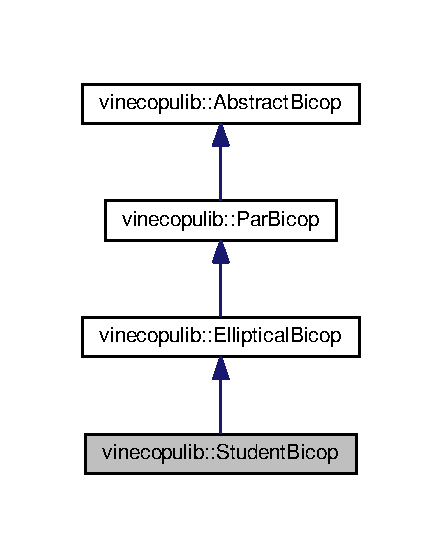
\includegraphics[width=212pt]{classvinecopulib_1_1_student_bicop__inherit__graph}
\end{center}
\end{figure}


Collaboration diagram for vinecopulib\+:\+:Student\+Bicop\+:\nopagebreak
\begin{figure}[H]
\begin{center}
\leavevmode
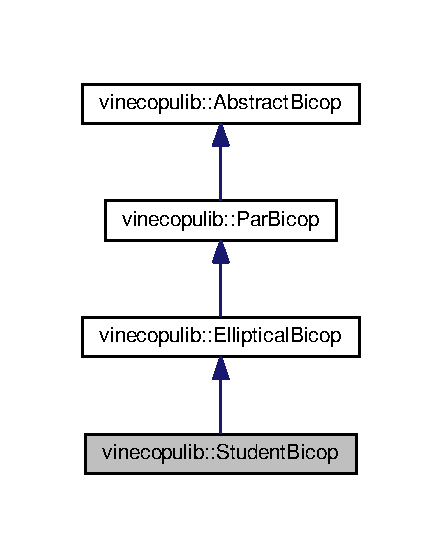
\includegraphics[width=212pt]{classvinecopulib_1_1_student_bicop__coll__graph}
\end{center}
\end{figure}
\subsection*{Additional Inherited Members}


\subsection{Detailed Description}
The Student t copula. 

This class is used in the implementation underlying the \hyperlink{classvinecopulib_1_1_bicop}{Bicop} class. Users should not use \hyperlink{classvinecopulib_1_1_abstract_bicop}{Abstract\+Bicop} or derived classes directly, but always work with the \hyperlink{classvinecopulib_1_1_bicop}{Bicop} interface.

Joe, Harry. Dependence modeling with copulas. C\+R\+C Press, 2014. 

The documentation for this class was generated from the following files\+:\begin{DoxyCompactItemize}
\item 
vinecopulib/include/vinecopulib/bicop/student.\+hpp\item 
vinecopulib/src/bicop/student.\+cpp\end{DoxyCompactItemize}

\hypertarget{classvinecopulib_1_1_tll0_bicop}{}\section{vinecopulib\+:\+:Tll0\+Bicop Class Reference}
\label{classvinecopulib_1_1_tll0_bicop}\index{vinecopulib\+::\+Tll0\+Bicop@{vinecopulib\+::\+Tll0\+Bicop}}


The transformation local-\/constant likelihood estimator.  




{\ttfamily \#include $<$tll0.\+hpp$>$}



Inheritance diagram for vinecopulib\+:\+:Tll0\+Bicop\+:
\nopagebreak
\begin{figure}[H]
\begin{center}
\leavevmode
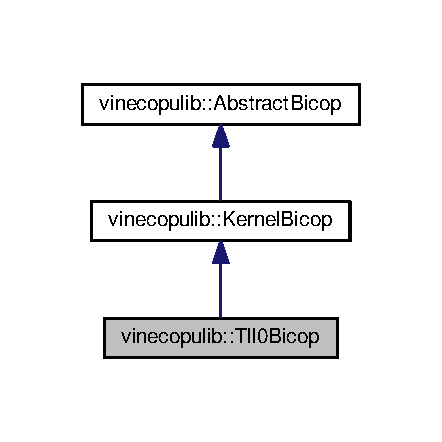
\includegraphics[width=213pt]{classvinecopulib_1_1_tll0_bicop__inherit__graph}
\end{center}
\end{figure}


Collaboration diagram for vinecopulib\+:\+:Tll0\+Bicop\+:
\nopagebreak
\begin{figure}[H]
\begin{center}
\leavevmode
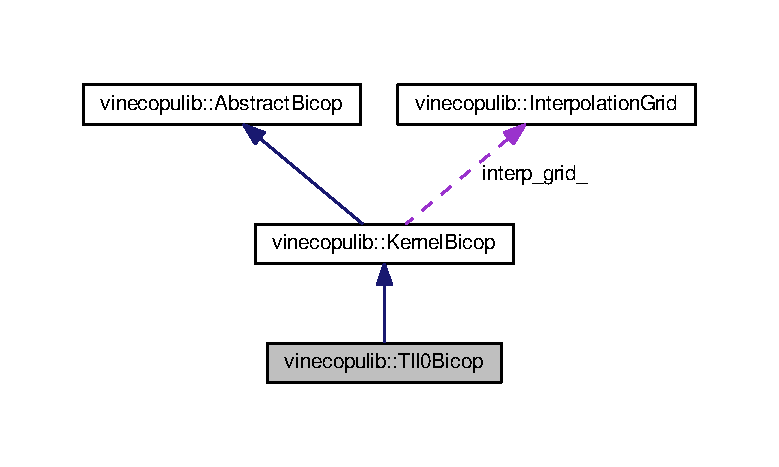
\includegraphics[width=350pt]{classvinecopulib_1_1_tll0_bicop__coll__graph}
\end{center}
\end{figure}
\subsection*{Additional Inherited Members}


\subsection{Detailed Description}
The transformation local-\/constant likelihood estimator. 

This class is used in the implementation underlying the \hyperlink{classvinecopulib_1_1_bicop}{Bicop} class. Users should not use \hyperlink{classvinecopulib_1_1_abstract_bicop}{Abstract\+Bicop} or derived classes directly, but always work with the \hyperlink{classvinecopulib_1_1_bicop}{Bicop} interface.

Nagler, Thomas. {\itshape kdecopula\+: An R Package for the Kernel Estimation of Copula Densities}. ar\+Xiv\+:1603.\+04229 \mbox{[}stat.\+CO\mbox{]}, 2016 

The documentation for this class was generated from the following files\+:\begin{DoxyCompactItemize}
\item 
/home/n5/dev/cpp/vinecopulib/include/bicop/tll0.\+hpp\item 
/home/n5/dev/cpp/vinecopulib/src/bicop/tll0.\+cpp\end{DoxyCompactItemize}

\hypertarget{classvinecopulib_1_1_vinecop}{}\section{vinecopulib\+:\+:Vinecop Class Reference}
\label{classvinecopulib_1_1_vinecop}\index{vinecopulib\+::\+Vinecop@{vinecopulib\+::\+Vinecop}}


A class for vine copula models.  




{\ttfamily \#include $<$class.\+hpp$>$}

\subsection*{Public Member Functions}
\begin{DoxyCompactItemize}
\item 
\hyperlink{classvinecopulib_1_1_vinecop_a391541e2795d06a848d5a17fe3496a63}{Vinecop} (size\+\_\+t d)
\item 
\hyperlink{classvinecopulib_1_1_vinecop_ab44ab72bb062123dabe8c1a5c569f0c0}{Vinecop} (const Eigen\+::\+Matrix$<$ size\+\_\+t, Eigen\+::\+Dynamic, Eigen\+::\+Dynamic $>$ \&matrix)
\item 
\hyperlink{classvinecopulib_1_1_vinecop_a4e6f60c2ddb191f0fe083dda346d0dd1}{Vinecop} (const std\+::vector$<$ std\+::vector$<$ \hyperlink{classvinecopulib_1_1_bicop}{Bicop} $>$$>$ \&pair\+\_\+copulas, const Eigen\+::\+Matrix$<$ size\+\_\+t, Eigen\+::\+Dynamic, Eigen\+::\+Dynamic $>$ \&matrix)
\item 
\hyperlink{classvinecopulib_1_1_vinecop_a1bba8d207a21b5d0c76660af40383822}{Vinecop} (const Eigen\+::\+Matrix\+Xd \&data, \hyperlink{classvinecopulib_1_1_fit_controls_vinecop}{Fit\+Controls\+Vinecop} controls=\hyperlink{classvinecopulib_1_1_fit_controls_vinecop}{Fit\+Controls\+Vinecop}())
\item 
\hyperlink{classvinecopulib_1_1_vinecop_a4c97ed6f0af4e4cb726a26629ad73c6b}{Vinecop} (const Eigen\+::\+Matrix\+Xd \&data, const Eigen\+::\+Matrix$<$ size\+\_\+t, Eigen\+::\+Dynamic, Eigen\+::\+Dynamic $>$ \&matrix, \hyperlink{classvinecopulib_1_1_fit_controls_vinecop}{Fit\+Controls\+Vinecop} controls=\hyperlink{classvinecopulib_1_1_fit_controls_vinecop}{Fit\+Controls\+Vinecop}())
\item 
void \hyperlink{classvinecopulib_1_1_vinecop_ad6cbb6b69c41f13a6e5e46ece44c0f78}{select\+\_\+all} (const Eigen\+::\+Matrix\+Xd \&data, \hyperlink{classvinecopulib_1_1_fit_controls_vinecop}{Fit\+Controls\+Vinecop} controls=\hyperlink{classvinecopulib_1_1_fit_controls_vinecop}{Fit\+Controls\+Vinecop}())
\item 
void \hyperlink{classvinecopulib_1_1_vinecop_a15ca60a0770dab0786b134fc80d1e77d}{select\+\_\+families} (const Eigen\+::\+Matrix\+Xd \&data, \hyperlink{classvinecopulib_1_1_fit_controls_vinecop}{Fit\+Controls\+Vinecop} controls=\hyperlink{classvinecopulib_1_1_fit_controls_vinecop}{Fit\+Controls\+Vinecop}())
\item 
Eigen\+::\+Vector\+Xd \hyperlink{classvinecopulib_1_1_vinecop_adf3760b8dd2b6d3a9cae5426188d4489}{pdf} (const Eigen\+::\+Matrix\+Xd \&u)
\item 
Eigen\+::\+Matrix\+Xd \hyperlink{classvinecopulib_1_1_vinecop_aa88f63a1fa62dce205c4c197d9deb152}{simulate} (size\+\_\+t n)
\item 
Eigen\+::\+Matrix\+Xd \hyperlink{classvinecopulib_1_1_vinecop_ac64ae8072851ea1cd4ed7143cac92933}{inverse\+\_\+rosenblatt} (const Eigen\+::\+Matrix\+Xd \&u)
\item 
double \hyperlink{classvinecopulib_1_1_vinecop_a507ad836872f9f702eed22ba25212515}{calculate\+\_\+npars} ()
\item 
double \hyperlink{classvinecopulib_1_1_vinecop_a53105af3a02ad07af454333733c21495}{loglik} (const Eigen\+::\+Matrix\+Xd \&u)
\item 
double \hyperlink{classvinecopulib_1_1_vinecop_afab8444e538c976fa601ab946dd76252}{aic} (const Eigen\+::\+Matrix\+Xd \&u)
\item 
double \hyperlink{classvinecopulib_1_1_vinecop_a3bee8adb75dee19687309a40bbd72000}{bic} (const Eigen\+::\+Matrix\+Xd \&u)
\end{DoxyCompactItemize}
\begin{Indent}{\bf Getters}\par
\begin{DoxyCompactItemize}
\item 
\hyperlink{classvinecopulib_1_1_bicop}{Bicop} \hyperlink{classvinecopulib_1_1_vinecop_aafcde16d37dbcef74af9158cdf525169}{get\+\_\+pair\+\_\+copula} (size\+\_\+t tree, size\+\_\+t edge) const 
\item 
\hyperlink{namespacevinecopulib_a42e95cc06d33896199caab0c11ad44f3}{Bicop\+Family} \hyperlink{classvinecopulib_1_1_vinecop_a4b27e03bb944bfc062b0aff2a6b540e8}{get\+\_\+family} (size\+\_\+t tree, size\+\_\+t edge) const 
\item 
int \hyperlink{classvinecopulib_1_1_vinecop_a985513046c1f06f6bcc1af376bae5e9d}{get\+\_\+rotation} (size\+\_\+t tree, size\+\_\+t edge) const 
\item 
Eigen\+::\+Vector\+Xd \hyperlink{classvinecopulib_1_1_vinecop_a96da7f2517bb19f7fe22c3380f3b4f26}{get\+\_\+parameters} (size\+\_\+t tree, size\+\_\+t edge) const 
\item 
Eigen\+::\+Matrix$<$ size\+\_\+t, Eigen\+::\+Dynamic, Eigen\+::\+Dynamic $>$ \hyperlink{classvinecopulib_1_1_vinecop_a615b96629e2c97299f0b904d8ccc5b76}{get\+\_\+matrix} () const \hypertarget{classvinecopulib_1_1_vinecop_a615b96629e2c97299f0b904d8ccc5b76}{}\label{classvinecopulib_1_1_vinecop_a615b96629e2c97299f0b904d8ccc5b76}

\begin{DoxyCompactList}\small\item\em extracts the structure matrix of the vine copula model. \end{DoxyCompactList}\item 
std\+::vector$<$ std\+::vector$<$ \hyperlink{classvinecopulib_1_1_bicop}{Bicop} $>$ $>$ \hyperlink{classvinecopulib_1_1_vinecop_acb041d08afd6b7efac4f3769273300d7}{get\+\_\+all\+\_\+pair\+\_\+copulas} () const 
\item 
std\+::vector$<$ std\+::vector$<$ \hyperlink{namespacevinecopulib_a42e95cc06d33896199caab0c11ad44f3}{Bicop\+Family} $>$ $>$ \hyperlink{classvinecopulib_1_1_vinecop_adcb572c440756a00dfaea0188caffb85}{get\+\_\+all\+\_\+families} () const 
\item 
std\+::vector$<$ std\+::vector$<$ int $>$ $>$ \hyperlink{classvinecopulib_1_1_vinecop_a7cbfca10a16e4c45f4b5d94343b5fc20}{get\+\_\+all\+\_\+rotations} () const 
\item 
std\+::vector$<$ std\+::vector$<$ Eigen\+::\+Vector\+Xd $>$ $>$ \hyperlink{classvinecopulib_1_1_vinecop_a3ab6a85281503d42f3a07036001bd657}{get\+\_\+all\+\_\+parameters} () const 
\end{DoxyCompactItemize}
\end{Indent}
\subsection*{Static Public Member Functions}
\begin{DoxyCompactItemize}
\item 
static std\+::vector$<$ std\+::vector$<$ \hyperlink{classvinecopulib_1_1_bicop}{Bicop} $>$ $>$ \hyperlink{classvinecopulib_1_1_vinecop_a44f2ca25c3e08fa0e185539d8d29f13b}{make\+\_\+pair\+\_\+copula\+\_\+store} (size\+\_\+t d)
\end{DoxyCompactItemize}


\subsection{Detailed Description}
A class for vine copula models. 

A vine copula model is characterized by the structure matrix (see \hyperlink{classvinecopulib_1_1_r_vine_matrix}{R\+Vine\+Matrix}) and the pair-\/copulas. 

\subsection{Constructor \& Destructor Documentation}
\index{vinecopulib\+::\+Vinecop@{vinecopulib\+::\+Vinecop}!Vinecop@{Vinecop}}
\index{Vinecop@{Vinecop}!vinecopulib\+::\+Vinecop@{vinecopulib\+::\+Vinecop}}
\subsubsection[{\texorpdfstring{Vinecop(size\+\_\+t d)}{Vinecop(size_t d)}}]{\setlength{\rightskip}{0pt plus 5cm}vinecopulib\+::\+Vinecop\+::\+Vinecop (
\begin{DoxyParamCaption}
\item[{size\+\_\+t}]{d}
\end{DoxyParamCaption}
)}\hypertarget{classvinecopulib_1_1_vinecop_a391541e2795d06a848d5a17fe3496a63}{}\label{classvinecopulib_1_1_vinecop_a391541e2795d06a848d5a17fe3496a63}
creates a D-\/vine on {\ttfamily d} variables with all pair-\/copulas set to independence. 
\begin{DoxyParams}{Parameters}
{\em d} & the dimension (= number of variables) of the model. \\
\hline
\end{DoxyParams}
\index{vinecopulib\+::\+Vinecop@{vinecopulib\+::\+Vinecop}!Vinecop@{Vinecop}}
\index{Vinecop@{Vinecop}!vinecopulib\+::\+Vinecop@{vinecopulib\+::\+Vinecop}}
\subsubsection[{\texorpdfstring{Vinecop(const Eigen\+::\+Matrix$<$ size\+\_\+t, Eigen\+::\+Dynamic, Eigen\+::\+Dynamic $>$ \&matrix)}{Vinecop(const Eigen::Matrix< size_t, Eigen::Dynamic, Eigen::Dynamic > &matrix)}}]{\setlength{\rightskip}{0pt plus 5cm}vinecopulib\+::\+Vinecop\+::\+Vinecop (
\begin{DoxyParamCaption}
\item[{const Eigen\+::\+Matrix$<$ size\+\_\+t, Eigen\+::\+Dynamic, Eigen\+::\+Dynamic $>$ \&}]{matrix}
\end{DoxyParamCaption}
)}\hypertarget{classvinecopulib_1_1_vinecop_ab44ab72bb062123dabe8c1a5c569f0c0}{}\label{classvinecopulib_1_1_vinecop_ab44ab72bb062123dabe8c1a5c569f0c0}
creates a vine copula with structure specified by an R-\/vine matrix; all pair-\/copulas are set to independence. 
\begin{DoxyParams}{Parameters}
{\em matrix} & an R-\/vine matrix. \\
\hline
\end{DoxyParams}
\index{vinecopulib\+::\+Vinecop@{vinecopulib\+::\+Vinecop}!Vinecop@{Vinecop}}
\index{Vinecop@{Vinecop}!vinecopulib\+::\+Vinecop@{vinecopulib\+::\+Vinecop}}
\subsubsection[{\texorpdfstring{Vinecop(const std\+::vector$<$ std\+::vector$<$ Bicop $>$$>$ \&pair\+\_\+copulas, const Eigen\+::\+Matrix$<$ size\+\_\+t, Eigen\+::\+Dynamic, Eigen\+::\+Dynamic $>$ \&matrix)}{Vinecop(const std::vector< std::vector< Bicop >> &pair_copulas, const Eigen::Matrix< size_t, Eigen::Dynamic, Eigen::Dynamic > &matrix)}}]{\setlength{\rightskip}{0pt plus 5cm}vinecopulib\+::\+Vinecop\+::\+Vinecop (
\begin{DoxyParamCaption}
\item[{const std\+::vector$<$ std\+::vector$<$ {\bf Bicop} $>$$>$ \&}]{pair\+\_\+copulas, }
\item[{const Eigen\+::\+Matrix$<$ size\+\_\+t, Eigen\+::\+Dynamic, Eigen\+::\+Dynamic $>$ \&}]{matrix}
\end{DoxyParamCaption}
)}\hypertarget{classvinecopulib_1_1_vinecop_a4e6f60c2ddb191f0fe083dda346d0dd1}{}\label{classvinecopulib_1_1_vinecop_a4e6f60c2ddb191f0fe083dda346d0dd1}
creates an arbitrary vine copula model. 
\begin{DoxyParams}{Parameters}
{\em pair\+\_\+copulas} & \hyperlink{classvinecopulib_1_1_bicop}{Bicop} objects specifying the pair-\/copulas, see \hyperlink{classvinecopulib_1_1_vinecop_a44f2ca25c3e08fa0e185539d8d29f13b}{make\+\_\+pair\+\_\+copula\+\_\+store()}. \\
\hline
{\em matrix} & an R-\/vine matrix specifying the vine structure. \\
\hline
\end{DoxyParams}
\index{vinecopulib\+::\+Vinecop@{vinecopulib\+::\+Vinecop}!Vinecop@{Vinecop}}
\index{Vinecop@{Vinecop}!vinecopulib\+::\+Vinecop@{vinecopulib\+::\+Vinecop}}
\subsubsection[{\texorpdfstring{Vinecop(const Eigen\+::\+Matrix\+Xd \&data, Fit\+Controls\+Vinecop controls=\+Fit\+Controls\+Vinecop())}{Vinecop(const Eigen::MatrixXd &data, FitControlsVinecop controls=FitControlsVinecop())}}]{\setlength{\rightskip}{0pt plus 5cm}vinecopulib\+::\+Vinecop\+::\+Vinecop (
\begin{DoxyParamCaption}
\item[{const Eigen\+::\+Matrix\+Xd \&}]{data, }
\item[{{\bf Fit\+Controls\+Vinecop}}]{controls = {\ttfamily {\bf Fit\+Controls\+Vinecop}()}}
\end{DoxyParamCaption}
)}\hypertarget{classvinecopulib_1_1_vinecop_a1bba8d207a21b5d0c76660af40383822}{}\label{classvinecopulib_1_1_vinecop_a1bba8d207a21b5d0c76660af40383822}
constructs a vine copula model from data.

The function creates a model and calls \hyperlink{classvinecopulib_1_1_vinecop_ad6cbb6b69c41f13a6e5e46ece44c0f78}{select\+\_\+all()}.


\begin{DoxyParams}{Parameters}
{\em data} & an $ n \times d $ matrix of observations. \\
\hline
{\em controls} & see \hyperlink{classvinecopulib_1_1_fit_controls_vinecop}{Fit\+Controls\+Vinecop}. \\
\hline
\end{DoxyParams}
\index{vinecopulib\+::\+Vinecop@{vinecopulib\+::\+Vinecop}!Vinecop@{Vinecop}}
\index{Vinecop@{Vinecop}!vinecopulib\+::\+Vinecop@{vinecopulib\+::\+Vinecop}}
\subsubsection[{\texorpdfstring{Vinecop(const Eigen\+::\+Matrix\+Xd \&data, const Eigen\+::\+Matrix$<$ size\+\_\+t, Eigen\+::\+Dynamic, Eigen\+::\+Dynamic $>$ \&matrix, Fit\+Controls\+Vinecop controls=\+Fit\+Controls\+Vinecop())}{Vinecop(const Eigen::MatrixXd &data, const Eigen::Matrix< size_t, Eigen::Dynamic, Eigen::Dynamic > &matrix, FitControlsVinecop controls=FitControlsVinecop())}}]{\setlength{\rightskip}{0pt plus 5cm}vinecopulib\+::\+Vinecop\+::\+Vinecop (
\begin{DoxyParamCaption}
\item[{const Eigen\+::\+Matrix\+Xd \&}]{data, }
\item[{const Eigen\+::\+Matrix$<$ size\+\_\+t, Eigen\+::\+Dynamic, Eigen\+::\+Dynamic $>$ \&}]{matrix, }
\item[{{\bf Fit\+Controls\+Vinecop}}]{controls = {\ttfamily {\bf Fit\+Controls\+Vinecop}()}}
\end{DoxyParamCaption}
)}\hypertarget{classvinecopulib_1_1_vinecop_a4c97ed6f0af4e4cb726a26629ad73c6b}{}\label{classvinecopulib_1_1_vinecop_a4c97ed6f0af4e4cb726a26629ad73c6b}
constructs a vine copula model from data.

The function creates a model and calls select\+\_\+family().


\begin{DoxyParams}{Parameters}
{\em data} & an $ n \times d $ matrix of observations. \\
\hline
{\em matrix} & either an empty matrix (default) or an R-\/vine structure matrix, see \hyperlink{classvinecopulib_1_1_vinecop_a15ca60a0770dab0786b134fc80d1e77d}{select\+\_\+families()}. \\
\hline
{\em controls} & see \hyperlink{classvinecopulib_1_1_fit_controls_vinecop}{Fit\+Controls\+Vinecop}. \\
\hline
\end{DoxyParams}


\subsection{Member Function Documentation}
\index{vinecopulib\+::\+Vinecop@{vinecopulib\+::\+Vinecop}!aic@{aic}}
\index{aic@{aic}!vinecopulib\+::\+Vinecop@{vinecopulib\+::\+Vinecop}}
\subsubsection[{\texorpdfstring{aic(const Eigen\+::\+Matrix\+Xd \&u)}{aic(const Eigen::MatrixXd &u)}}]{\setlength{\rightskip}{0pt plus 5cm}double vinecopulib\+::\+Vinecop\+::aic (
\begin{DoxyParamCaption}
\item[{const Eigen\+::\+Matrix\+Xd \&}]{u}
\end{DoxyParamCaption}
)}\hypertarget{classvinecopulib_1_1_vinecop_afab8444e538c976fa601ab946dd76252}{}\label{classvinecopulib_1_1_vinecop_afab8444e538c976fa601ab946dd76252}
calculates the Akaike information criterion (A\+IC).

The A\+IC is defined as \[ \mathrm{AIC} = -2\, \mathrm{loglik} + 2 p, \] where $ \mathrm{loglik} $ is the log-\/liklihood and $ p $ is the (effective) number of parameters of the model, see \hyperlink{classvinecopulib_1_1_vinecop_a53105af3a02ad07af454333733c21495}{loglik()} and \hyperlink{classvinecopulib_1_1_vinecop_a507ad836872f9f702eed22ba25212515}{calculate\+\_\+npars()}. The A\+IC is a consistent model selection criterion for nonparametric models.


\begin{DoxyParams}{Parameters}
{\em u} & $n \times 2$ matrix of observations. \\
\hline
\end{DoxyParams}
\index{vinecopulib\+::\+Vinecop@{vinecopulib\+::\+Vinecop}!bic@{bic}}
\index{bic@{bic}!vinecopulib\+::\+Vinecop@{vinecopulib\+::\+Vinecop}}
\subsubsection[{\texorpdfstring{bic(const Eigen\+::\+Matrix\+Xd \&u)}{bic(const Eigen::MatrixXd &u)}}]{\setlength{\rightskip}{0pt plus 5cm}double vinecopulib\+::\+Vinecop\+::bic (
\begin{DoxyParamCaption}
\item[{const Eigen\+::\+Matrix\+Xd \&}]{u}
\end{DoxyParamCaption}
)}\hypertarget{classvinecopulib_1_1_vinecop_a3bee8adb75dee19687309a40bbd72000}{}\label{classvinecopulib_1_1_vinecop_a3bee8adb75dee19687309a40bbd72000}
calculates the Bayesian information criterion (B\+IC).

The B\+IC is defined as \[ \mathrm{BIC} = -2\, \mathrm{loglik} + \ln(n) p, \] where $ \mathrm{loglik} $ is the log-\/liklihood and $ p $ is the (effective) number of parameters of the model, see \hyperlink{classvinecopulib_1_1_vinecop_a53105af3a02ad07af454333733c21495}{loglik()} and \hyperlink{classvinecopulib_1_1_vinecop_a507ad836872f9f702eed22ba25212515}{calculate\+\_\+npars()}. The B\+IC is a consistent model selection criterion for nonparametric models.


\begin{DoxyParams}{Parameters}
{\em u} & $n \times 2$ matrix of observations. \\
\hline
\end{DoxyParams}
\index{vinecopulib\+::\+Vinecop@{vinecopulib\+::\+Vinecop}!calculate\+\_\+npars@{calculate\+\_\+npars}}
\index{calculate\+\_\+npars@{calculate\+\_\+npars}!vinecopulib\+::\+Vinecop@{vinecopulib\+::\+Vinecop}}
\subsubsection[{\texorpdfstring{calculate\+\_\+npars()}{calculate_npars()}}]{\setlength{\rightskip}{0pt plus 5cm}double vinecopulib\+::\+Vinecop\+::calculate\+\_\+npars (
\begin{DoxyParamCaption}
{}
\end{DoxyParamCaption}
)}\hypertarget{classvinecopulib_1_1_vinecop_a507ad836872f9f702eed22ba25212515}{}\label{classvinecopulib_1_1_vinecop_a507ad836872f9f702eed22ba25212515}
calculates the effective number of parameters.

Returns sum of the number of parameters for all pair copulas (see \hyperlink{classvinecopulib_1_1_bicop_a9f3b3b83c54a9e1d809fdee058f3eb11}{Bicop\+::calculate\+\_\+npars()}). \index{vinecopulib\+::\+Vinecop@{vinecopulib\+::\+Vinecop}!get\+\_\+all\+\_\+families@{get\+\_\+all\+\_\+families}}
\index{get\+\_\+all\+\_\+families@{get\+\_\+all\+\_\+families}!vinecopulib\+::\+Vinecop@{vinecopulib\+::\+Vinecop}}
\subsubsection[{\texorpdfstring{get\+\_\+all\+\_\+families() const }{get_all_families() const }}]{\setlength{\rightskip}{0pt plus 5cm}std\+::vector$<$ std\+::vector$<$ {\bf Bicop\+Family} $>$ $>$ vinecopulib\+::\+Vinecop\+::get\+\_\+all\+\_\+families (
\begin{DoxyParamCaption}
{}
\end{DoxyParamCaption}
) const}\hypertarget{classvinecopulib_1_1_vinecop_adcb572c440756a00dfaea0188caffb85}{}\label{classvinecopulib_1_1_vinecop_adcb572c440756a00dfaea0188caffb85}
extracts the families of all pair copulas.

\begin{DoxyReturn}{Returns}
a nested std\+::vector with entry {\ttfamily \mbox{[}t\mbox{]}\mbox{[}e\mbox{]}} corresponding to edge {\ttfamily e} in tree {\ttfamily t}. 
\end{DoxyReturn}
\index{vinecopulib\+::\+Vinecop@{vinecopulib\+::\+Vinecop}!get\+\_\+all\+\_\+pair\+\_\+copulas@{get\+\_\+all\+\_\+pair\+\_\+copulas}}
\index{get\+\_\+all\+\_\+pair\+\_\+copulas@{get\+\_\+all\+\_\+pair\+\_\+copulas}!vinecopulib\+::\+Vinecop@{vinecopulib\+::\+Vinecop}}
\subsubsection[{\texorpdfstring{get\+\_\+all\+\_\+pair\+\_\+copulas() const }{get_all_pair_copulas() const }}]{\setlength{\rightskip}{0pt plus 5cm}std\+::vector$<$ std\+::vector$<$ {\bf Bicop} $>$ $>$ vinecopulib\+::\+Vinecop\+::get\+\_\+all\+\_\+pair\+\_\+copulas (
\begin{DoxyParamCaption}
{}
\end{DoxyParamCaption}
) const}\hypertarget{classvinecopulib_1_1_vinecop_acb041d08afd6b7efac4f3769273300d7}{}\label{classvinecopulib_1_1_vinecop_acb041d08afd6b7efac4f3769273300d7}
extracts all pair copulas.

\begin{DoxyReturn}{Returns}
a nested std\+::vector with entry {\ttfamily \mbox{[}t\mbox{]}\mbox{[}e\mbox{]}} corresponding to edge {\ttfamily e} in tree {\ttfamily t}. 
\end{DoxyReturn}
\index{vinecopulib\+::\+Vinecop@{vinecopulib\+::\+Vinecop}!get\+\_\+all\+\_\+parameters@{get\+\_\+all\+\_\+parameters}}
\index{get\+\_\+all\+\_\+parameters@{get\+\_\+all\+\_\+parameters}!vinecopulib\+::\+Vinecop@{vinecopulib\+::\+Vinecop}}
\subsubsection[{\texorpdfstring{get\+\_\+all\+\_\+parameters() const }{get_all_parameters() const }}]{\setlength{\rightskip}{0pt plus 5cm}std\+::vector$<$ std\+::vector$<$ Eigen\+::\+Vector\+Xd $>$ $>$ vinecopulib\+::\+Vinecop\+::get\+\_\+all\+\_\+parameters (
\begin{DoxyParamCaption}
{}
\end{DoxyParamCaption}
) const}\hypertarget{classvinecopulib_1_1_vinecop_a3ab6a85281503d42f3a07036001bd657}{}\label{classvinecopulib_1_1_vinecop_a3ab6a85281503d42f3a07036001bd657}
extracts the parameters of all pair copulas.

\begin{DoxyReturn}{Returns}
a nested std\+::vector with entry {\ttfamily \mbox{[}t\mbox{]}\mbox{[}e\mbox{]}} corresponding to edge {\ttfamily e} in tree {\ttfamily t}. 
\end{DoxyReturn}
\index{vinecopulib\+::\+Vinecop@{vinecopulib\+::\+Vinecop}!get\+\_\+all\+\_\+rotations@{get\+\_\+all\+\_\+rotations}}
\index{get\+\_\+all\+\_\+rotations@{get\+\_\+all\+\_\+rotations}!vinecopulib\+::\+Vinecop@{vinecopulib\+::\+Vinecop}}
\subsubsection[{\texorpdfstring{get\+\_\+all\+\_\+rotations() const }{get_all_rotations() const }}]{\setlength{\rightskip}{0pt plus 5cm}std\+::vector$<$ std\+::vector$<$ int $>$ $>$ vinecopulib\+::\+Vinecop\+::get\+\_\+all\+\_\+rotations (
\begin{DoxyParamCaption}
{}
\end{DoxyParamCaption}
) const}\hypertarget{classvinecopulib_1_1_vinecop_a7cbfca10a16e4c45f4b5d94343b5fc20}{}\label{classvinecopulib_1_1_vinecop_a7cbfca10a16e4c45f4b5d94343b5fc20}
extracts the rotations of all pair copulas.

\begin{DoxyReturn}{Returns}
a nested std\+::vector with entry {\ttfamily \mbox{[}t\mbox{]}\mbox{[}e\mbox{]}} corresponding to edge {\ttfamily e} in tree {\ttfamily t}. 
\end{DoxyReturn}
\index{vinecopulib\+::\+Vinecop@{vinecopulib\+::\+Vinecop}!get\+\_\+family@{get\+\_\+family}}
\index{get\+\_\+family@{get\+\_\+family}!vinecopulib\+::\+Vinecop@{vinecopulib\+::\+Vinecop}}
\subsubsection[{\texorpdfstring{get\+\_\+family(size\+\_\+t tree, size\+\_\+t edge) const }{get_family(size_t tree, size_t edge) const }}]{\setlength{\rightskip}{0pt plus 5cm}{\bf Bicop\+Family} vinecopulib\+::\+Vinecop\+::get\+\_\+family (
\begin{DoxyParamCaption}
\item[{size\+\_\+t}]{tree, }
\item[{size\+\_\+t}]{edge}
\end{DoxyParamCaption}
) const}\hypertarget{classvinecopulib_1_1_vinecop_a4b27e03bb944bfc062b0aff2a6b540e8}{}\label{classvinecopulib_1_1_vinecop_a4b27e03bb944bfc062b0aff2a6b540e8}
extracts the family of a pair copula.


\begin{DoxyParams}{Parameters}
{\em tree} & tree index (starting with 0). \\
\hline
{\em edge} & edge index (starting with 0). \\
\hline
\end{DoxyParams}
\index{vinecopulib\+::\+Vinecop@{vinecopulib\+::\+Vinecop}!get\+\_\+pair\+\_\+copula@{get\+\_\+pair\+\_\+copula}}
\index{get\+\_\+pair\+\_\+copula@{get\+\_\+pair\+\_\+copula}!vinecopulib\+::\+Vinecop@{vinecopulib\+::\+Vinecop}}
\subsubsection[{\texorpdfstring{get\+\_\+pair\+\_\+copula(size\+\_\+t tree, size\+\_\+t edge) const }{get_pair_copula(size_t tree, size_t edge) const }}]{\setlength{\rightskip}{0pt plus 5cm}{\bf Bicop} vinecopulib\+::\+Vinecop\+::get\+\_\+pair\+\_\+copula (
\begin{DoxyParamCaption}
\item[{size\+\_\+t}]{tree, }
\item[{size\+\_\+t}]{edge}
\end{DoxyParamCaption}
) const}\hypertarget{classvinecopulib_1_1_vinecop_aafcde16d37dbcef74af9158cdf525169}{}\label{classvinecopulib_1_1_vinecop_aafcde16d37dbcef74af9158cdf525169}
extracts a pair copula.


\begin{DoxyParams}{Parameters}
{\em tree} & tree index (starting with 0). \\
\hline
{\em edge} & edge index (starting with 0). \\
\hline
\end{DoxyParams}
\index{vinecopulib\+::\+Vinecop@{vinecopulib\+::\+Vinecop}!get\+\_\+parameters@{get\+\_\+parameters}}
\index{get\+\_\+parameters@{get\+\_\+parameters}!vinecopulib\+::\+Vinecop@{vinecopulib\+::\+Vinecop}}
\subsubsection[{\texorpdfstring{get\+\_\+parameters(size\+\_\+t tree, size\+\_\+t edge) const }{get_parameters(size_t tree, size_t edge) const }}]{\setlength{\rightskip}{0pt plus 5cm}Eigen\+::\+Vector\+Xd vinecopulib\+::\+Vinecop\+::get\+\_\+parameters (
\begin{DoxyParamCaption}
\item[{size\+\_\+t}]{tree, }
\item[{size\+\_\+t}]{edge}
\end{DoxyParamCaption}
) const}\hypertarget{classvinecopulib_1_1_vinecop_a96da7f2517bb19f7fe22c3380f3b4f26}{}\label{classvinecopulib_1_1_vinecop_a96da7f2517bb19f7fe22c3380f3b4f26}
extracts the parameters of a pair copula.


\begin{DoxyParams}{Parameters}
{\em tree} & tree index (starting with 0). \\
\hline
{\em edge} & edge index (starting with 0). \\
\hline
\end{DoxyParams}
\index{vinecopulib\+::\+Vinecop@{vinecopulib\+::\+Vinecop}!get\+\_\+rotation@{get\+\_\+rotation}}
\index{get\+\_\+rotation@{get\+\_\+rotation}!vinecopulib\+::\+Vinecop@{vinecopulib\+::\+Vinecop}}
\subsubsection[{\texorpdfstring{get\+\_\+rotation(size\+\_\+t tree, size\+\_\+t edge) const }{get_rotation(size_t tree, size_t edge) const }}]{\setlength{\rightskip}{0pt plus 5cm}int vinecopulib\+::\+Vinecop\+::get\+\_\+rotation (
\begin{DoxyParamCaption}
\item[{size\+\_\+t}]{tree, }
\item[{size\+\_\+t}]{edge}
\end{DoxyParamCaption}
) const}\hypertarget{classvinecopulib_1_1_vinecop_a985513046c1f06f6bcc1af376bae5e9d}{}\label{classvinecopulib_1_1_vinecop_a985513046c1f06f6bcc1af376bae5e9d}
extracts the rotation of a pair copula.


\begin{DoxyParams}{Parameters}
{\em tree} & tree index (starting with 0). \\
\hline
{\em edge} & edge index (starting with 0). \\
\hline
\end{DoxyParams}
\index{vinecopulib\+::\+Vinecop@{vinecopulib\+::\+Vinecop}!inverse\+\_\+rosenblatt@{inverse\+\_\+rosenblatt}}
\index{inverse\+\_\+rosenblatt@{inverse\+\_\+rosenblatt}!vinecopulib\+::\+Vinecop@{vinecopulib\+::\+Vinecop}}
\subsubsection[{\texorpdfstring{inverse\+\_\+rosenblatt(const Eigen\+::\+Matrix\+Xd \&u)}{inverse_rosenblatt(const Eigen::MatrixXd &u)}}]{\setlength{\rightskip}{0pt plus 5cm}Eigen\+::\+Matrix\+Xd vinecopulib\+::\+Vinecop\+::inverse\+\_\+rosenblatt (
\begin{DoxyParamCaption}
\item[{const Eigen\+::\+Matrix\+Xd \&}]{u}
\end{DoxyParamCaption}
)}\hypertarget{classvinecopulib_1_1_vinecop_ac64ae8072851ea1cd4ed7143cac92933}{}\label{classvinecopulib_1_1_vinecop_ac64ae8072851ea1cd4ed7143cac92933}
calculates the inverse Rosenblatt transform for a vine copula model.

The inverse Rosenblatt transform can be used for simulation\+: the function applied to independent uniform variates resembles simulated data from the vine copula model.

If the problem is too large, it is split recursively into halves (w.\+r.\+t. n, the number of observations). \char`\"{}\+Too large\char`\"{} means that the required memory will exceed 1 GB. An examplary configuration requiring less than 1 GB is $ n = 1000 $, $d = 200$.


\begin{DoxyParams}{Parameters}
{\em u} & $ n \times d $ matrix of evaluation points. \\
\hline
\end{DoxyParams}
\index{vinecopulib\+::\+Vinecop@{vinecopulib\+::\+Vinecop}!loglik@{loglik}}
\index{loglik@{loglik}!vinecopulib\+::\+Vinecop@{vinecopulib\+::\+Vinecop}}
\subsubsection[{\texorpdfstring{loglik(const Eigen\+::\+Matrix\+Xd \&u)}{loglik(const Eigen::MatrixXd &u)}}]{\setlength{\rightskip}{0pt plus 5cm}double vinecopulib\+::\+Vinecop\+::loglik (
\begin{DoxyParamCaption}
\item[{const Eigen\+::\+Matrix\+Xd \&}]{u}
\end{DoxyParamCaption}
)}\hypertarget{classvinecopulib_1_1_vinecop_a53105af3a02ad07af454333733c21495}{}\label{classvinecopulib_1_1_vinecop_a53105af3a02ad07af454333733c21495}
calculates the log-\/likelihood.

The log-\/likelihood is defined as \[ \mathrm{loglik} = \sum_{i = 1}^n \ln c(U_{1, i}, ..., U_{d, i}), \] where $ c $ is the copula density \hyperlink{classvinecopulib_1_1_vinecop_adf3760b8dd2b6d3a9cae5426188d4489}{pdf()}.


\begin{DoxyParams}{Parameters}
{\em u} & $n \times d$ matrix of observations. \\
\hline
\end{DoxyParams}
\index{vinecopulib\+::\+Vinecop@{vinecopulib\+::\+Vinecop}!make\+\_\+pair\+\_\+copula\+\_\+store@{make\+\_\+pair\+\_\+copula\+\_\+store}}
\index{make\+\_\+pair\+\_\+copula\+\_\+store@{make\+\_\+pair\+\_\+copula\+\_\+store}!vinecopulib\+::\+Vinecop@{vinecopulib\+::\+Vinecop}}
\subsubsection[{\texorpdfstring{make\+\_\+pair\+\_\+copula\+\_\+store(size\+\_\+t d)}{make_pair_copula_store(size_t d)}}]{\setlength{\rightskip}{0pt plus 5cm}std\+::vector$<$ std\+::vector$<$ {\bf Bicop} $>$ $>$ vinecopulib\+::\+Vinecop\+::make\+\_\+pair\+\_\+copula\+\_\+store (
\begin{DoxyParamCaption}
\item[{size\+\_\+t}]{d}
\end{DoxyParamCaption}
)\hspace{0.3cm}{\ttfamily [static]}}\hypertarget{classvinecopulib_1_1_vinecop_a44f2ca25c3e08fa0e185539d8d29f13b}{}\label{classvinecopulib_1_1_vinecop_a44f2ca25c3e08fa0e185539d8d29f13b}
Initialize object for storing pair copulas


\begin{DoxyParams}{Parameters}
{\em d} & dimension of the vine copula. \\
\hline
\end{DoxyParams}
\begin{DoxyReturn}{Returns}
A nested vector such that {\ttfamily pc\+\_\+store\mbox{[}t\mbox{]}\mbox{[}e\mbox{]}} contains a \hyperlink{classvinecopulib_1_1_bicop}{Bicop} object for the pair copula corresponding to tree {\ttfamily t} and edge {\ttfamily e}. 
\end{DoxyReturn}
\index{vinecopulib\+::\+Vinecop@{vinecopulib\+::\+Vinecop}!pdf@{pdf}}
\index{pdf@{pdf}!vinecopulib\+::\+Vinecop@{vinecopulib\+::\+Vinecop}}
\subsubsection[{\texorpdfstring{pdf(const Eigen\+::\+Matrix\+Xd \&u)}{pdf(const Eigen::MatrixXd &u)}}]{\setlength{\rightskip}{0pt plus 5cm}Eigen\+::\+Vector\+Xd vinecopulib\+::\+Vinecop\+::pdf (
\begin{DoxyParamCaption}
\item[{const Eigen\+::\+Matrix\+Xd \&}]{u}
\end{DoxyParamCaption}
)}\hypertarget{classvinecopulib_1_1_vinecop_adf3760b8dd2b6d3a9cae5426188d4489}{}\label{classvinecopulib_1_1_vinecop_adf3760b8dd2b6d3a9cae5426188d4489}
calculates the density function of the vine copula model.


\begin{DoxyParams}{Parameters}
{\em u} & $ n \times d $ matrix of evaluation points. \\
\hline
\end{DoxyParams}
\index{vinecopulib\+::\+Vinecop@{vinecopulib\+::\+Vinecop}!select\+\_\+all@{select\+\_\+all}}
\index{select\+\_\+all@{select\+\_\+all}!vinecopulib\+::\+Vinecop@{vinecopulib\+::\+Vinecop}}
\subsubsection[{\texorpdfstring{select\+\_\+all(const Eigen\+::\+Matrix\+Xd \&data, Fit\+Controls\+Vinecop controls=\+Fit\+Controls\+Vinecop())}{select_all(const Eigen::MatrixXd &data, FitControlsVinecop controls=FitControlsVinecop())}}]{\setlength{\rightskip}{0pt plus 5cm}void vinecopulib\+::\+Vinecop\+::select\+\_\+all (
\begin{DoxyParamCaption}
\item[{const Eigen\+::\+Matrix\+Xd \&}]{data, }
\item[{{\bf Fit\+Controls\+Vinecop}}]{controls = {\ttfamily {\bf Fit\+Controls\+Vinecop}()}}
\end{DoxyParamCaption}
)}\hypertarget{classvinecopulib_1_1_vinecop_ad6cbb6b69c41f13a6e5e46ece44c0f78}{}\label{classvinecopulib_1_1_vinecop_ad6cbb6b69c41f13a6e5e46ece44c0f78}
automatically fits and selects a vine copula model

Selection of the structure is performed using the algorithm of Dissmann, J. F., E. C. Brechmann, C. Czado, and D. Kurowicka (2013). {\itshape Selecting and estimating regular vine copulae and application to financial returns.} Computational Statistics \& Data Analysis, 59 (1), 52-\/69.


\begin{DoxyParams}{Parameters}
{\em data} & nxd matrix of copula data. \\
\hline
{\em controls} & the controls to the algorithm (see \hyperlink{classvinecopulib_1_1_fit_controls_vinecop}{Fit\+Controls\+Vinecop}). \\
\hline
\end{DoxyParams}
\index{vinecopulib\+::\+Vinecop@{vinecopulib\+::\+Vinecop}!select\+\_\+families@{select\+\_\+families}}
\index{select\+\_\+families@{select\+\_\+families}!vinecopulib\+::\+Vinecop@{vinecopulib\+::\+Vinecop}}
\subsubsection[{\texorpdfstring{select\+\_\+families(const Eigen\+::\+Matrix\+Xd \&data, Fit\+Controls\+Vinecop controls=\+Fit\+Controls\+Vinecop())}{select_families(const Eigen::MatrixXd &data, FitControlsVinecop controls=FitControlsVinecop())}}]{\setlength{\rightskip}{0pt plus 5cm}void vinecopulib\+::\+Vinecop\+::select\+\_\+families (
\begin{DoxyParamCaption}
\item[{const Eigen\+::\+Matrix\+Xd \&}]{data, }
\item[{{\bf Fit\+Controls\+Vinecop}}]{controls = {\ttfamily {\bf Fit\+Controls\+Vinecop}()}}
\end{DoxyParamCaption}
)}\hypertarget{classvinecopulib_1_1_vinecop_a15ca60a0770dab0786b134fc80d1e77d}{}\label{classvinecopulib_1_1_vinecop_a15ca60a0770dab0786b134fc80d1e77d}
automatically selects all pair-\/copula families and fits all parameters.


\begin{DoxyParams}{Parameters}
{\em data} & nxd matrix of copula data. \\
\hline
{\em controls} & the controls to the algorithm (see \hyperlink{classvinecopulib_1_1_fit_controls_vinecop}{Fit\+Controls\+Vinecop}). \\
\hline
\end{DoxyParams}
\index{vinecopulib\+::\+Vinecop@{vinecopulib\+::\+Vinecop}!simulate@{simulate}}
\index{simulate@{simulate}!vinecopulib\+::\+Vinecop@{vinecopulib\+::\+Vinecop}}
\subsubsection[{\texorpdfstring{simulate(size\+\_\+t n)}{simulate(size_t n)}}]{\setlength{\rightskip}{0pt plus 5cm}Eigen\+::\+Matrix\+Xd vinecopulib\+::\+Vinecop\+::simulate (
\begin{DoxyParamCaption}
\item[{size\+\_\+t}]{n}
\end{DoxyParamCaption}
)}\hypertarget{classvinecopulib_1_1_vinecop_aa88f63a1fa62dce205c4c197d9deb152}{}\label{classvinecopulib_1_1_vinecop_aa88f63a1fa62dce205c4c197d9deb152}
simulates from a vine copula model, see \hyperlink{classvinecopulib_1_1_vinecop_ac64ae8072851ea1cd4ed7143cac92933}{inverse\+\_\+rosenblatt()}.


\begin{DoxyParams}{Parameters}
{\em n} & number of observations. \\
\hline
\end{DoxyParams}


The documentation for this class was generated from the following files\+:\begin{DoxyCompactItemize}
\item 
/home/n5/dev/cpp/vinecopulib/include/vinecopulib/vinecop/class.\+hpp\item 
/home/n5/dev/cpp/vinecopulib/src/vinecop/class.\+cpp\end{DoxyCompactItemize}

\chapter{File Documentation}
\hypertarget{mainpage_8h}{}\section{vinecopulib/include/mainpage.h File Reference}
\label{mainpage_8h}\index{vinecopulib/include/mainpage.\+h@{vinecopulib/include/mainpage.\+h}}


api\+\_\+docs  




\subsection{Detailed Description}
api\+\_\+docs 


\hypertarget{family_8hpp}{}\section{/home/n5/dev/cpp/vinecopulib/include/bicop/family.hpp File Reference}
\label{family_8hpp}\index{/home/n5/dev/cpp/vinecopulib/include/bicop/family.\+hpp@{/home/n5/dev/cpp/vinecopulib/include/bicop/family.\+hpp}}
{\ttfamily \#include $<$vector$>$}\\*
{\ttfamily \#include $<$string$>$}\\*
Include dependency graph for family.\+hpp\+:
\nopagebreak
\begin{figure}[H]
\begin{center}
\leavevmode
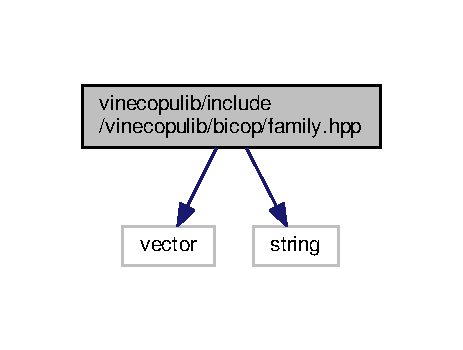
\includegraphics[width=226pt]{family_8hpp__incl}
\end{center}
\end{figure}
This graph shows which files directly or indirectly include this file\+:
\nopagebreak
\begin{figure}[H]
\begin{center}
\leavevmode
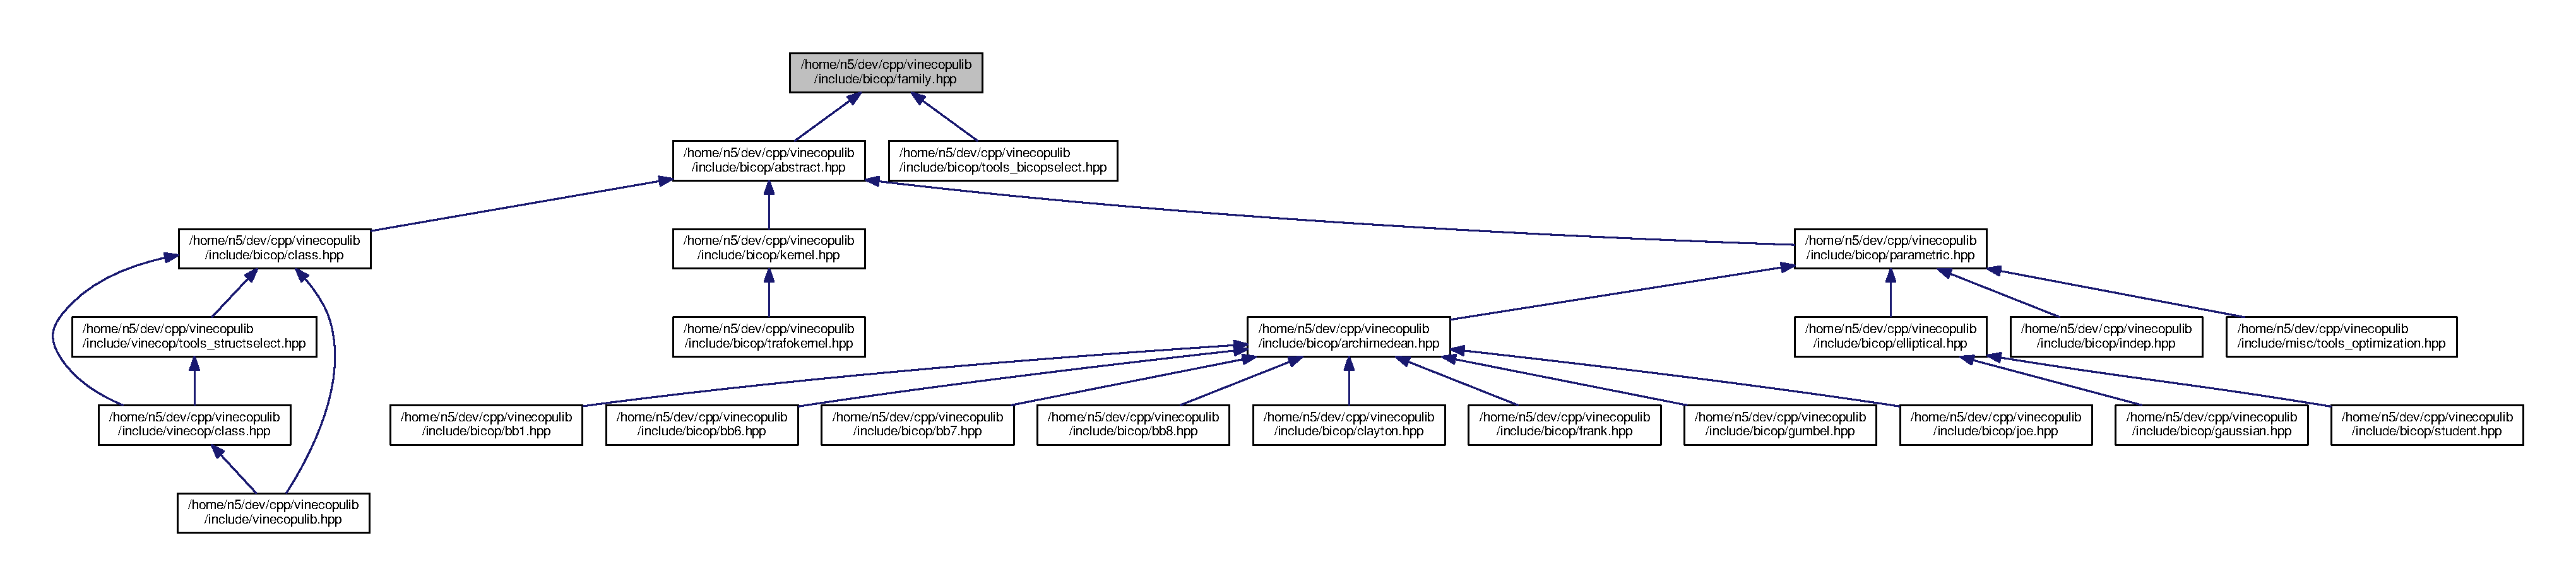
\includegraphics[width=350pt]{family_8hpp__dep__incl}
\end{center}
\end{figure}
\subsection*{Namespaces}
\begin{DoxyCompactItemize}
\item 
 \hyperlink{namespacevinecopulib}{vinecopulib}
\begin{DoxyCompactList}\small\item\em Tools for bivariate and vine copula modeling. \end{DoxyCompactList}\item 
 \hyperlink{namespacevinecopulib_1_1bicop__families}{vinecopulib\+::bicop\+\_\+families}
\begin{DoxyCompactList}\small\item\em Convenience definitions of sets of bivariate copula families. \end{DoxyCompactList}\end{DoxyCompactItemize}
\subsection*{Enumerations}
\begin{DoxyCompactItemize}
\item 
enum \hyperlink{namespacevinecopulib_a42e95cc06d33896199caab0c11ad44f3}{vinecopulib\+::\+Bicop\+Family} \{ \\*
\hyperlink{namespacevinecopulib_a42e95cc06d33896199caab0c11ad44f3af49b022096e968010a7b9bd941805a65}{vinecopulib\+::\+Bicop\+Family\+::indep}, 
\\*
\hyperlink{namespacevinecopulib_a42e95cc06d33896199caab0c11ad44f3a304e2a3b544f6b9f267a151e1bcee487}{vinecopulib\+::\+Bicop\+Family\+::gaussian}, 
\\*
\hyperlink{namespacevinecopulib_a42e95cc06d33896199caab0c11ad44f3acd73502828457d15655bbd7a63fb0bc8}{vinecopulib\+::\+Bicop\+Family\+::student}, 
\\*
\hyperlink{namespacevinecopulib_a42e95cc06d33896199caab0c11ad44f3ad0b8c94bb241f6f7a4b96cd6d3e26c36}{vinecopulib\+::\+Bicop\+Family\+::clayton}, 
\\*
\hyperlink{namespacevinecopulib_a42e95cc06d33896199caab0c11ad44f3a7bfb9d9ee5abbfa800e56bbe62db9bbe}{vinecopulib\+::\+Bicop\+Family\+::gumbel}, 
\\*
\hyperlink{namespacevinecopulib_a42e95cc06d33896199caab0c11ad44f3a26253c50741faa9c2e2b836773c69fe6}{vinecopulib\+::\+Bicop\+Family\+::frank}, 
\\*
\hyperlink{namespacevinecopulib_a42e95cc06d33896199caab0c11ad44f3a8ff32489f92f33416694be8fdc2d4c22}{vinecopulib\+::\+Bicop\+Family\+::joe}, 
\\*
\hyperlink{namespacevinecopulib_a42e95cc06d33896199caab0c11ad44f3a8a2e0a5eece6b7020e5308bcd0df4aa3}{vinecopulib\+::\+Bicop\+Family\+::bb1}, 
\\*
\hyperlink{namespacevinecopulib_a42e95cc06d33896199caab0c11ad44f3aa2d33c13012f342a80bdc94b60538c68}{vinecopulib\+::\+Bicop\+Family\+::bb6}, 
\\*
\hyperlink{namespacevinecopulib_a42e95cc06d33896199caab0c11ad44f3ac9e791d6604a5fcc1f4e6ad574f43328}{vinecopulib\+::\+Bicop\+Family\+::bb7}, 
\\*
\hyperlink{namespacevinecopulib_a42e95cc06d33896199caab0c11ad44f3adf8b15ba30764e3b9ce084c11336603a}{vinecopulib\+::\+Bicop\+Family\+::bb8}, 
\\*
\hyperlink{namespacevinecopulib_a42e95cc06d33896199caab0c11ad44f3acd36652e61e82e7935de462b329cc8e6}{vinecopulib\+::\+Bicop\+Family\+::tll0}
 \}\begin{DoxyCompactList}\small\item\em A bivariate copula family identifier. \end{DoxyCompactList}
\end{DoxyCompactItemize}
\subsection*{Functions}
\begin{DoxyCompactItemize}
\item 
std\+::string \hyperlink{namespacevinecopulib_ac46553ae5f99072f65e9d3254d2c526d}{vinecopulib\+::get\+\_\+family\+\_\+name} (Bicop\+Family family)
\end{DoxyCompactItemize}
\subsection*{Variables}
\begin{DoxyCompactItemize}
\item 
const std\+::vector$<$ Bicop\+Family $>$ \hyperlink{namespacevinecopulib_1_1bicop__families_a5214a513f41ec23b74782aab96ea6774}{vinecopulib\+::bicop\+\_\+families\+::all}
\begin{DoxyCompactList}\small\item\em All implemented families. \end{DoxyCompactList}\item 
const std\+::vector$<$ Bicop\+Family $>$ \hyperlink{namespacevinecopulib_1_1bicop__families_a76d66bb6cb03ae4de1cef3d1ed70ac16}{vinecopulib\+::bicop\+\_\+families\+::parametric}
\begin{DoxyCompactList}\small\item\em All parametric families. \end{DoxyCompactList}\item 
const std\+::vector$<$ Bicop\+Family $>$ \hyperlink{namespacevinecopulib_1_1bicop__families_a01c7c990cc34b1b74d115858a52fcdc5}{vinecopulib\+::bicop\+\_\+families\+::nonparametric}
\begin{DoxyCompactList}\small\item\em All nonparametric families. \end{DoxyCompactList}\item 
const std\+::vector$<$ Bicop\+Family $>$ \hyperlink{namespacevinecopulib_1_1bicop__families_aba503484b0a13cfb0e67c026e2f295d4}{vinecopulib\+::bicop\+\_\+families\+::one\+\_\+par}
\begin{DoxyCompactList}\small\item\em All one-\/parameter families. \end{DoxyCompactList}\item 
const std\+::vector$<$ Bicop\+Family $>$ \hyperlink{namespacevinecopulib_1_1bicop__families_ad5871c39b4ee62bd44fa851d7d70c7ca}{vinecopulib\+::bicop\+\_\+families\+::two\+\_\+par}
\begin{DoxyCompactList}\small\item\em All two-\/parameter families. \end{DoxyCompactList}\item 
const std\+::vector$<$ Bicop\+Family $>$ \hyperlink{namespacevinecopulib_1_1bicop__families_a24b790671c9f4b25e57ecbc3505232fb}{vinecopulib\+::bicop\+\_\+families\+::elliptical}
\begin{DoxyCompactList}\small\item\em All elliptical copulas. \end{DoxyCompactList}\item 
const std\+::vector$<$ Bicop\+Family $>$ \hyperlink{namespacevinecopulib_1_1bicop__families_a714863b69ae59ac48c7fb2be45cd2619}{vinecopulib\+::bicop\+\_\+families\+::archimedean}
\begin{DoxyCompactList}\small\item\em All Archimedean copulas. \end{DoxyCompactList}\item 
const std\+::vector$<$ Bicop\+Family $>$ \hyperlink{namespacevinecopulib_1_1bicop__families_aea9f7383b4bbbe47d4862f25e6bb8ad8}{vinecopulib\+::bicop\+\_\+families\+::\+BB}
\begin{DoxyCompactList}\small\item\em All BB copulas. \end{DoxyCompactList}\item 
const std\+::vector$<$ Bicop\+Family $>$ \hyperlink{namespacevinecopulib_1_1bicop__families_ac221bc84c32d2836692ed40d89439928}{vinecopulib\+::bicop\+\_\+families\+::rotationless}
\item 
const std\+::vector$<$ Bicop\+Family $>$ \hyperlink{namespacevinecopulib_1_1bicop__families_a5a5f349f07638768ff8b1bb2ae90d102}{vinecopulib\+::bicop\+\_\+families\+::lt}
\begin{DoxyCompactList}\small\item\em Families with stronger dependence in the lower tail. \end{DoxyCompactList}\item 
const std\+::vector$<$ Bicop\+Family $>$ \hyperlink{namespacevinecopulib_1_1bicop__families_af754a2d2697709c204dda0473215f9cd}{vinecopulib\+::bicop\+\_\+families\+::ut}
\begin{DoxyCompactList}\small\item\em Families with stronger dependence in the upper tail. \end{DoxyCompactList}\item 
const std\+::vector$<$ Bicop\+Family $>$ \hyperlink{namespacevinecopulib_1_1bicop__families_af92a2e71f03e2280276533def655760d}{vinecopulib\+::bicop\+\_\+families\+::itau}
\begin{DoxyCompactList}\small\item\em Families for which {\ttfamily method = \char`\"{}itau\char`\"{}} is available in \hyperlink{classvinecopulib_1_1_bicop_a2d509a8b404a73ef17f04a0678e90a71}{Bicop\+::fit()} \end{DoxyCompactList}\item 
const std\+::vector$<$ Bicop\+Family $>$ \hyperlink{namespacevinecopulib_1_1bicop__families_ae1ae1673e3d4a9c57bd9df074e17a3b9}{vinecopulib\+::bicop\+\_\+families\+::flip\+\_\+by\+\_\+rotation}
\begin{DoxyCompactList}\small\item\em Families that can be flipped by adjusting the rotation. \end{DoxyCompactList}\end{DoxyCompactItemize}

\hypertarget{tools__stats_8cpp}{}\section{/home/n5/dev/cpp/vinecopulib/src/misc/tools\+\_\+stats.cpp File Reference}
\label{tools__stats_8cpp}\index{/home/n5/dev/cpp/vinecopulib/src/misc/tools\+\_\+stats.\+cpp@{/home/n5/dev/cpp/vinecopulib/src/misc/tools\+\_\+stats.\+cpp}}
{\ttfamily \#include \char`\"{}misc/tools\+\_\+stats.\+hpp\char`\"{}}\\*
{\ttfamily \#include \char`\"{}misc/tools\+\_\+stl.\+hpp\char`\"{}}\\*
{\ttfamily \#include \char`\"{}misc/tools\+\_\+c.\+h\char`\"{}}\\*
Include dependency graph for tools\+\_\+stats.\+cpp\+:
\nopagebreak
\begin{figure}[H]
\begin{center}
\leavevmode
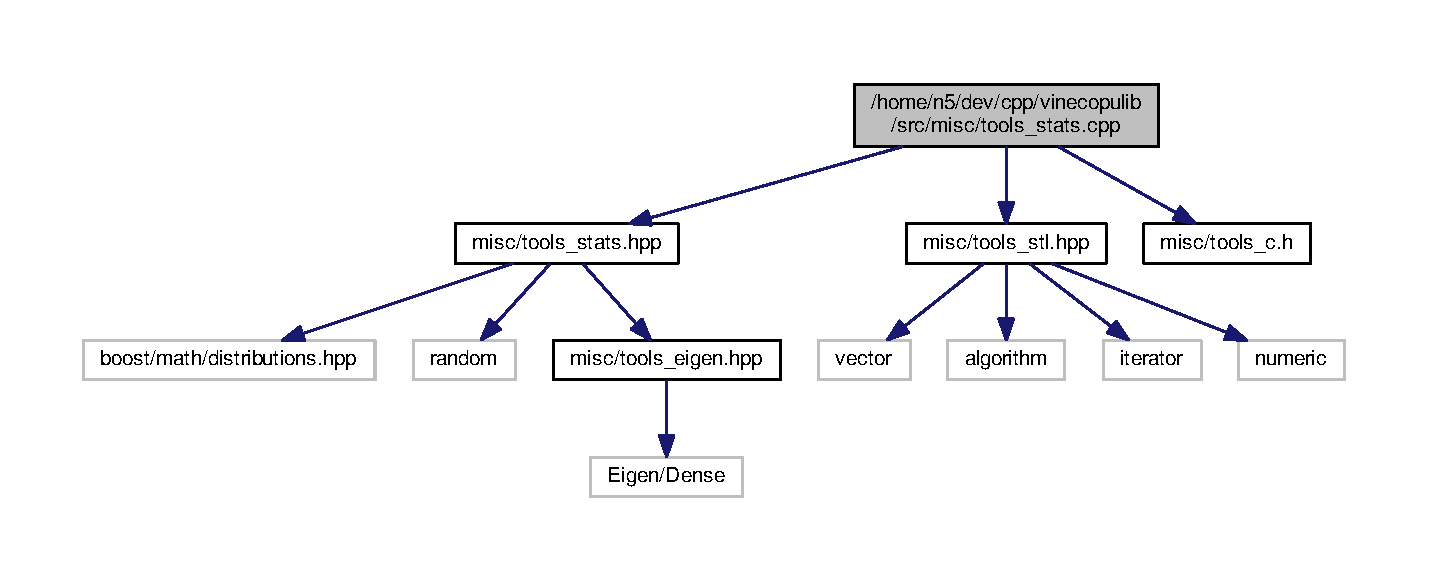
\includegraphics[width=350pt]{tools__stats_8cpp__incl}
\end{center}
\end{figure}
\subsection*{Namespaces}
\begin{DoxyCompactItemize}
\item 
 \hyperlink{namespacetools__stats}{tools\+\_\+stats}
\begin{DoxyCompactList}\small\item\em Utilities for statistical analysis. \end{DoxyCompactList}\end{DoxyCompactItemize}
\subsection*{Functions}
\begin{DoxyCompactItemize}
\item 
Eigen\+::\+Matrix\+Xd \hyperlink{namespacetools__stats_ad857f9c70a10a498f3c449225500f4c0}{tools\+\_\+stats\+::simulate\+\_\+uniform} (int n, int d)
\item 
Eigen\+::\+Matrix\+Xd \hyperlink{namespacetools__stats_a88048bc643d51f30f099c33eb2f61598}{tools\+\_\+stats\+::to\+\_\+pseudo\+\_\+obs} (Eigen\+::\+Matrix\+Xd x, std\+::string ties\+\_\+method)
\item 
Eigen\+::\+Vector\+Xd \hyperlink{namespacetools__stats_af09c24563535c110aea492a30eed3d3e}{tools\+\_\+stats\+::to\+\_\+pseudo\+\_\+obs\+\_\+1d} (Eigen\+::\+Vector\+Xd x, std\+::string ties\+\_\+method)
\end{DoxyCompactItemize}
\begin{Indent}{\bf Pairwise dependence measures}\par
{\em 
\begin{DoxyParams}{Parameters}
{\em x} & an $ n \times 2 $ matrix of observations. \\
\hline
\end{DoxyParams}
}\begin{DoxyCompactItemize}
\item 
double \hyperlink{namespacetools__stats_aba1c21a7a90e6fefb3d92876469f401e}{tools\+\_\+stats\+::pairwise\+\_\+ktau} (Eigen\+::\+Matrix$<$ double, Eigen\+::\+Dynamic, 2 $>$ \&x)\hypertarget{namespacetools__stats_aba1c21a7a90e6fefb3d92876469f401e}{}\label{namespacetools__stats_aba1c21a7a90e6fefb3d92876469f401e}

\begin{DoxyCompactList}\small\item\em calculates the pairwise Kendall\textquotesingle{}s $ \tau $. \end{DoxyCompactList}\item 
double \hyperlink{namespacetools__stats_ada062011e2c2a18d7258a39ad0722b7e}{tools\+\_\+stats\+::pairwise\+\_\+cor} (const Eigen\+::\+Matrix$<$ double, Eigen\+::\+Dynamic, 2 $>$ \&x)\hypertarget{namespacetools__stats_ada062011e2c2a18d7258a39ad0722b7e}{}\label{namespacetools__stats_ada062011e2c2a18d7258a39ad0722b7e}

\begin{DoxyCompactList}\small\item\em calculates the pairwise correlation. \end{DoxyCompactList}\item 
double \hyperlink{namespacetools__stats_a937dc78ae41420f0726847d94016ba86}{tools\+\_\+stats\+::pairwise\+\_\+hoeffd} (Eigen\+::\+Matrix$<$ double, Eigen\+::\+Dynamic, 2 $>$ x)\hypertarget{namespacetools__stats_a937dc78ae41420f0726847d94016ba86}{}\label{namespacetools__stats_a937dc78ae41420f0726847d94016ba86}

\begin{DoxyCompactList}\small\item\em calculates the pair-\/wise Hoeffding\textquotesingle{}s D. \end{DoxyCompactList}\end{DoxyCompactItemize}
\end{Indent}

%--- End generated contents ---

% Index
\newpage
\phantomsection
\addcontentsline{toc}{chapter}{Index}
\printindex

\end{document}
